%  LaTeX support: latex@mdpi.com
%  For support, please attach all files needed for compiling as well as the log file, and specify your operating system, LaTeX version, and LaTeX editor.

%=================================================================
% pandoc conditionals added to preserve backwards compatibility with previous versions of rticles

\documentclass[notspecified,article,submit,moreauthors,pdftex]{Definitions/mdpi}


%% Some pieces required from the pandoc template
\setlist[itemize]{leftmargin=*,labelsep=5.8mm}
\setlist[enumerate]{leftmargin=*,labelsep=4.9mm}


%--------------------
% Class Options:
%--------------------

%---------
% article
%---------
% The default type of manuscript is "article", but can be replaced by:
% abstract, addendum, article, book, bookreview, briefreport, casereport, comment, commentary, communication, conferenceproceedings, correction, conferencereport, entry, expressionofconcern, extendedabstract, datadescriptor, editorial, essay, erratum, hypothesis, interestingimage, obituary, opinion, projectreport, reply, retraction, review, perspective, protocol, shortnote, studyprotocol, systematicreview, supfile, technicalnote, viewpoint, guidelines, registeredreport, tutorial
% supfile = supplementary materials

%----------
% submit
%----------
% The class option "submit" will be changed to "accept" by the Editorial Office when the paper is accepted. This will only make changes to the frontpage (e.g., the logo of the journal will get visible), the headings, and the copyright information. Also, line numbering will be removed. Journal info and pagination for accepted papers will also be assigned by the Editorial Office.

%------------------
% moreauthors
%------------------
% If there is only one author the class option oneauthor should be used. Otherwise use the class option moreauthors.

%---------
% pdftex
%---------
% The option pdftex is for use with pdfLaTeX. Remove "pdftex" for (1) compiling with LaTeX & dvi2pdf (if eps figures are used) or for (2) compiling with XeLaTeX.

%=================================================================
% MDPI internal commands - do not modify
\firstpage{1}
\makeatletter
\setcounter{page}{\@firstpage}
\makeatother
\pubvolume{1}
\issuenum{1}
\articlenumber{0}
\pubyear{2023}
\copyrightyear{2023}
%\externaleditor{Academic Editor: Firstname Lastname}
\datereceived{ }
\daterevised{ } % Comment out if no revised date
\dateaccepted{ }
\datepublished{ }
%\datecorrected{} % For corrected papers: "Corrected: XXX" date in the original paper.
%\dateretracted{} % For corrected papers: "Retracted: XXX" date in the original paper.
\hreflink{https://doi.org/} % If needed use \linebreak
%\doinum{}
%\pdfoutput=1 % Uncommented for upload to arXiv.org

%=================================================================
% Add packages and commands here. The following packages are loaded in our class file: fontenc, inputenc, calc, indentfirst, fancyhdr, graphicx, epstopdf, lastpage, ifthen, float, amsmath, amssymb, lineno, setspace, enumitem, mathpazo, booktabs, titlesec, etoolbox, tabto, xcolor, colortbl, soul, multirow, microtype, tikz, totcount, changepage, attrib, upgreek, array, tabularx, pbox, ragged2e, tocloft, marginnote, marginfix, enotez, amsthm, natbib, hyperref, cleveref, scrextend, url, geometry, newfloat, caption, draftwatermark, seqsplit
% cleveref: load \crefname definitions after \begin{document}

%=================================================================
% Please use the following mathematics environments: Theorem, Lemma, Corollary, Proposition, Characterization, Property, Problem, Example, ExamplesandDefinitions, Hypothesis, Remark, Definition, Notation, Assumption
%% For proofs, please use the proof environment (the amsthm package is loaded by the MDPI class).

%=================================================================
% Full title of the paper (Capitalized)
\Title{Full title of the paper (Capitalized)}

% MDPI internal command: Title for citation in the left column
\TitleCitation{Full title of the paper (Capitalized)}

% Author Orchid ID: enter ID or remove command
%\newcommand{\orcidauthorA}{0000-0000-0000-000X} % Add \orcidA{} behind the author's name
%\newcommand{\orcidauthorB}{0000-0000-0000-000X} % Add \orcidB{} behind the author's name


% Authors, for the paper (add full first names)
\Author{Dominik
Leutnant$^{1,2,\ddagger,*}$\href{https://orcid.org/0000-0003-3293-2315}
{\orcidicon}, John Doe$^{2, \dagger, \ddagger}$}


%\longauthorlist{yes}


% MDPI internal command: Authors, for metadata in PDF
\AuthorNames{Dominik Leutnant, John Doe}

% MDPI internal command: Authors, for citation in the left column
%\AuthorCitation{Lastname, F.; Lastname, F.; Lastname, F.}
% If this is a Chicago style journal: Lastname, Firstname, Firstname Lastname, and Firstname Lastname.
\AuthorCitation{Leutnant, D.; Doe, J.}

% Affiliations / Addresses (Add [1] after \address if there is only one affiliation.)
\address{%
$^{1}$ \quad Muenster University of Applied Sciences - Institute for
Infrastructure, Water, Resources, Environment Correnstr. 25, 48149
Muenster,
Germany; \href{mailto:leutnant@fh-muenster.de}{\nolinkurl{leutnant@fh-muenster.de}}\\
$^{2}$ \quad Your department Street, City,
Country; \href{mailto:mail@mail.com}{\nolinkurl{mail@mail.com}}\\
}

% Contact information of the corresponding author
\corres{Correspondence: \href{mailto:leutnant@fh-muenster.de}{\nolinkurl{leutnant@fh-muenster.de}};
Tel.: +XX-000-00-0000.}

% Current address and/or shared authorship
\firstnote{Current address: Updated affiliation}
\secondnote{These authors contributed equally to this work.}






% The commands \thirdnote{} till \eighthnote{} are available for further notes

% Simple summary
\simplesumm{A Simple summary goes here.}

%\conference{} % An extended version of a conference paper

% Abstract (Do not insert blank lines, i.e. \\)
\abstract{A single paragraph of about 200 words maximum. For research
articles, abstracts should give a pertinent overview of the work. We
strongly encourage authors to use the following style of structured
abstracts, but without headings: 1) Background: Place the question
addressed in a broad context and highlight the purpose of the study; 2)
Methods: Describe briefly the main methods or treatments applied; 3)
Results: Summarize the article's main findings; and 4) Conclusion:
Indicate the main conclusions or interpretations. The abstract should be
an objective representation of the article, it must not contain results
which are not presented and substantiated in the main text and should
not exaggerate the main conclusions.}


% Keywords
\keyword{keyword 1; keyword 2; keyword 3 (list three to ten pertinent
keywords specific to the article, yet reasonably common within the
subject discipline.).}

% The fields PACS, MSC, and JEL may be left empty or commented out if not applicable
%\PACS{J0101}
%\MSC{}
%\JEL{}

%%%%%%%%%%%%%%%%%%%%%%%%%%%%%%%%%%%%%%%%%%
% Only for the journal Diversity
%\LSID{\url{http://}}

%%%%%%%%%%%%%%%%%%%%%%%%%%%%%%%%%%%%%%%%%%
% Only for the journal Applied Sciences

%%%%%%%%%%%%%%%%%%%%%%%%%%%%%%%%%%%%%%%%%%

%%%%%%%%%%%%%%%%%%%%%%%%%%%%%%%%%%%%%%%%%%
% Only for the journal Data



%%%%%%%%%%%%%%%%%%%%%%%%%%%%%%%%%%%%%%%%%%
% Only for the journal Toxins


%%%%%%%%%%%%%%%%%%%%%%%%%%%%%%%%%%%%%%%%%%
% Only for the journal Encyclopedia


%%%%%%%%%%%%%%%%%%%%%%%%%%%%%%%%%%%%%%%%%%
% Only for the journal Advances in Respiratory Medicine
%\addhighlights{yes}
%\renewcommand{\addhighlights}{%

%\noindent This is an obligatory section in “Advances in Respiratory Medicine”, whose goal is to increase the discoverability and readability of the article via search engines and other scholars. Highlights should not be a copy of the abstract, but a simple text allowing the reader to quickly and simplified find out what the article is about and what can be cited from it. Each of these parts should be devoted up to 2~bullet points.\vspace{3pt}\\
%\textbf{What are the main findings?}
% \begin{itemize}[labelsep=2.5mm,topsep=-3pt]
% \item First bullet.
% \item Second bullet.
% \end{itemize}\vspace{3pt}
%\textbf{What is the implication of the main finding?}
% \begin{itemize}[labelsep=2.5mm,topsep=-3pt]
% \item First bullet.
% \item Second bullet.
% \end{itemize}
%}


%%%%%%%%%%%%%%%%%%%%%%%%%%%%%%%%%%%%%%%%%%

% Pandoc syntax highlighting
\usepackage{color}
\usepackage{fancyvrb}
\newcommand{\VerbBar}{|}
\newcommand{\VERB}{\Verb[commandchars=\\\{\}]}
\DefineVerbatimEnvironment{Highlighting}{Verbatim}{commandchars=\\\{\}}
% Add ',fontsize=\small' for more characters per line
\usepackage{framed}
\definecolor{shadecolor}{RGB}{248,248,248}
\newenvironment{Shaded}{\begin{snugshade}}{\end{snugshade}}
\newcommand{\AlertTok}[1]{\textcolor[rgb]{0.94,0.16,0.16}{#1}}
\newcommand{\AnnotationTok}[1]{\textcolor[rgb]{0.56,0.35,0.01}{\textbf{\textit{#1}}}}
\newcommand{\AttributeTok}[1]{\textcolor[rgb]{0.13,0.29,0.53}{#1}}
\newcommand{\BaseNTok}[1]{\textcolor[rgb]{0.00,0.00,0.81}{#1}}
\newcommand{\BuiltInTok}[1]{#1}
\newcommand{\CharTok}[1]{\textcolor[rgb]{0.31,0.60,0.02}{#1}}
\newcommand{\CommentTok}[1]{\textcolor[rgb]{0.56,0.35,0.01}{\textit{#1}}}
\newcommand{\CommentVarTok}[1]{\textcolor[rgb]{0.56,0.35,0.01}{\textbf{\textit{#1}}}}
\newcommand{\ConstantTok}[1]{\textcolor[rgb]{0.56,0.35,0.01}{#1}}
\newcommand{\ControlFlowTok}[1]{\textcolor[rgb]{0.13,0.29,0.53}{\textbf{#1}}}
\newcommand{\DataTypeTok}[1]{\textcolor[rgb]{0.13,0.29,0.53}{#1}}
\newcommand{\DecValTok}[1]{\textcolor[rgb]{0.00,0.00,0.81}{#1}}
\newcommand{\DocumentationTok}[1]{\textcolor[rgb]{0.56,0.35,0.01}{\textbf{\textit{#1}}}}
\newcommand{\ErrorTok}[1]{\textcolor[rgb]{0.64,0.00,0.00}{\textbf{#1}}}
\newcommand{\ExtensionTok}[1]{#1}
\newcommand{\FloatTok}[1]{\textcolor[rgb]{0.00,0.00,0.81}{#1}}
\newcommand{\FunctionTok}[1]{\textcolor[rgb]{0.13,0.29,0.53}{\textbf{#1}}}
\newcommand{\ImportTok}[1]{#1}
\newcommand{\InformationTok}[1]{\textcolor[rgb]{0.56,0.35,0.01}{\textbf{\textit{#1}}}}
\newcommand{\KeywordTok}[1]{\textcolor[rgb]{0.13,0.29,0.53}{\textbf{#1}}}
\newcommand{\NormalTok}[1]{#1}
\newcommand{\OperatorTok}[1]{\textcolor[rgb]{0.81,0.36,0.00}{\textbf{#1}}}
\newcommand{\OtherTok}[1]{\textcolor[rgb]{0.56,0.35,0.01}{#1}}
\newcommand{\PreprocessorTok}[1]{\textcolor[rgb]{0.56,0.35,0.01}{\textit{#1}}}
\newcommand{\RegionMarkerTok}[1]{#1}
\newcommand{\SpecialCharTok}[1]{\textcolor[rgb]{0.81,0.36,0.00}{\textbf{#1}}}
\newcommand{\SpecialStringTok}[1]{\textcolor[rgb]{0.31,0.60,0.02}{#1}}
\newcommand{\StringTok}[1]{\textcolor[rgb]{0.31,0.60,0.02}{#1}}
\newcommand{\VariableTok}[1]{\textcolor[rgb]{0.00,0.00,0.00}{#1}}
\newcommand{\VerbatimStringTok}[1]{\textcolor[rgb]{0.31,0.60,0.02}{#1}}
\newcommand{\WarningTok}[1]{\textcolor[rgb]{0.56,0.35,0.01}{\textbf{\textit{#1}}}}

% tightlist command for lists without linebreak
\providecommand{\tightlist}{%
  \setlength{\itemsep}{0pt}\setlength{\parskip}{0pt}}



\usepackage{longtable}
\usepackage{booktabs}
\usepackage{array}
\usepackage{multirow}
\usepackage{wrapfig}
\usepackage{float}
\usepackage{colortbl}
\usepackage{pdflscape}
\usepackage{tabu}
\usepackage{threeparttable}
\usepackage{threeparttablex}
\usepackage[normalem]{ulem}
\usepackage{makecell}
\usepackage{xcolor}

\begin{document}



%%%%%%%%%%%%%%%%%%%%%%%%%%%%%%%%%%%%%%%%%%

\hypertarget{carga-de-libreruxedas}{%
\section{Carga de librerías}\label{carga-de-libreruxedas}}

\begin{Shaded}
\begin{Highlighting}[]
\FunctionTok{library}\NormalTok{(pacman)}
\NormalTok{packages }\OtherTok{=} \FunctionTok{c}\NormalTok{(}\StringTok{"MASS"}\NormalTok{,}\StringTok{"knitr"}\NormalTok{,}\StringTok{"tidyverse"}\NormalTok{,}\StringTok{"car"}\NormalTok{,}\StringTok{\textquotesingle{}dplyr\textquotesingle{}}\NormalTok{,}\StringTok{\textquotesingle{}kableExtra\textquotesingle{}}\NormalTok{,}\StringTok{"tidyr"}\NormalTok{,}\StringTok{"readr"}\NormalTok{,}\StringTok{"magrittr"}\NormalTok{,}\StringTok{"VIM"}\NormalTok{,}\StringTok{"GGally"}\NormalTok{,}\StringTok{"igraph"}\NormalTok{,}\StringTok{"ggplot2"}\NormalTok{,}\StringTok{"sf"}\NormalTok{,}\StringTok{"leaflet"}\NormalTok{,}\StringTok{"webshot2"}\NormalTok{)}
\NormalTok{pacman}\SpecialCharTok{::}\FunctionTok{p\_load}\NormalTok{(}\AttributeTok{char=}\NormalTok{packages)}
\end{Highlighting}
\end{Shaded}

\hypertarget{carga-de-ficheros}{%
\section{Carga de ficheros}\label{carga-de-ficheros}}

Para crear el dataset con el que vamos a tratar en este proyecto, hemos
extraido varios archivos de la
\href{https://valencia.opendatasoft.com/pages/home/}{web} del portal de
datos abiertos del Ayuntamiento de Valencia. En ellos tenemos diferente
información acerca de los 88 barrios que hay en Valencia, como pueden
ser el número de zonas verdes, precio del alquiler, actividad comercial,
renta, etc. Antes de atacar las preguntas que nuestro conjunto
resolverá, vamos a cargar los datos y unirlos en un único dataset, con
una variable común para todos, el barrio.

\hypertarget{vulnerabilidad}{%
\subsection{Vulnerabilidad}\label{vulnerabilidad}}

El primer dataset
\href{https://valencia.opendatasoft.com/explore/dataset/vulnerabilidad/table/}{Vulnerabilidad}
nos da información general del barrio, como la densidad de población, la
renta media, o el estado de vulnerabilidad. Esta última variable será de
gran interés en nuestro análisis posterior.

\begin{Shaded}
\begin{Highlighting}[]
\NormalTok{vuln }\OtherTok{\textless{}{-}} \FunctionTok{read\_delim}\NormalTok{(}\StringTok{"./data/vulnerabilidad.csv"}\NormalTok{, }
    \AttributeTok{delim =} \StringTok{";"}\NormalTok{, }\AttributeTok{escape\_double =} \ConstantTok{FALSE}\NormalTok{, }\AttributeTok{col\_types =} \FunctionTok{cols}\NormalTok{(}\StringTok{\textasciigrave{}}\AttributeTok{Geo Point}\StringTok{\textasciigrave{}} \OtherTok{=} \FunctionTok{col\_skip}\NormalTok{(), }
        \StringTok{\textasciigrave{}}\AttributeTok{Geo Shape}\StringTok{\textasciigrave{}} \OtherTok{=} \FunctionTok{col\_skip}\NormalTok{(), }\StringTok{\textasciigrave{}}\AttributeTok{Densitat\_p}\StringTok{\textasciigrave{}} \OtherTok{=} \FunctionTok{col\_skip}\NormalTok{()), }
    \AttributeTok{trim\_ws =} \ConstantTok{TRUE}\NormalTok{)}\SpecialCharTok{\%\textgreater{}\%}\FunctionTok{arrange}\NormalTok{(nombre)}

\FunctionTok{colnames}\NormalTok{(vuln)[}\FunctionTok{colnames}\NormalTok{(vuln) }\SpecialCharTok{==} \StringTok{"nombre"}\NormalTok{] }\OtherTok{\textless{}{-}}\StringTok{"Barrio"}
\FunctionTok{colnames}\NormalTok{(vuln)[}\FunctionTok{colnames}\NormalTok{(vuln) }\SpecialCharTok{==} \StringTok{"Index\_Gl\_1"}\NormalTok{] }\OtherTok{\textless{}{-}}\StringTok{"Indice\_Vuln"}


\NormalTok{vuln}\SpecialCharTok{$}\NormalTok{Barrio}\OtherTok{\textless{}{-}}\FunctionTok{factor}\NormalTok{(vuln}\SpecialCharTok{$}\NormalTok{Barrio,}\AttributeTok{levels =} \FunctionTok{unique}\NormalTok{(vuln}\SpecialCharTok{$}\NormalTok{Barrio))}
\NormalTok{vuln}\SpecialCharTok{$}\NormalTok{Indice\_Vuln}\OtherTok{\textless{}{-}}\FunctionTok{factor}\NormalTok{(vuln}\SpecialCharTok{$}\NormalTok{Indice\_Vuln,}\AttributeTok{levels =} \FunctionTok{c}\NormalTok{(}\StringTok{"Vulnerable"}\NormalTok{,}\StringTok{"Pot. Vulnerable"}\NormalTok{,}\StringTok{"No Vulnerable"}\NormalTok{))}

\FunctionTok{head}\NormalTok{(vuln)}
\end{Highlighting}
\end{Shaded}

\begin{verbatim}
# A tibble: 6 x 13
  Barrio      coddistbar coddistrit codbar `Zones verd` turismes_e atur_16_64 renda_mitj risc_pobre
  <fct>       <chr>           <dbl>  <dbl>        <dbl>      <dbl>      <dbl>      <dbl>      <dbl>
1 AIORA       121                12    121         1786       12.2     180.       10228.       24.3
2 ALBORS      122                12    122          712       12.2      63.6      11500        21.0
3 ARRANCAPINS 034                 3     34         1826       11.7     135.       15599.       14.7
4 BENICALAP   161                16    161         6999       11.7     301.       10256.       24.8
5 BENIFARAIG  171                17    171          521       11.9       7.45     10361        17.4
6 BENIFERRI   182                18    182           NA       NA        NA           NA        NA  
# i 4 more variables: Index_Equi <dbl>, Index_Soci <dbl>, Index_Glob <dbl>, Indice_Vuln <fct>
\end{verbatim}

Podemos ver en el código que es importante transformar la variable
\texttt{Barrio} en un factor, para poder graficar y tratar la
información de forma adecuada. Repetiremos este proceso en cada conjunto
de datos, además de poner a todos el mismo nombre para poder unirlos más
adelante.

\hypertarget{poblaciuxf3n}{%
\subsection{Población}\label{poblaciuxf3n}}

Este conjunto contiene el area y la población de los diferentes barrios.
Hemos considerado este dataset debido a que los datos de areas y
densidad de población que nos proporcionaba el conjunto vulnerabilidad y
barrios no cuadraban con nuestras búsquedas y carecían de sentido. Por
ello hemos considerado este otro que se ajusta mucho mejor. Para
calcular la densidad usaremos la función mutate.

\begin{Shaded}
\begin{Highlighting}[]
\FunctionTok{load}\NormalTok{(}\StringTok{"./data/Demografico.RData"}\NormalTok{)}

\FunctionTok{colnames}\NormalTok{(demografico)[}\FunctionTok{colnames}\NormalTok{(demografico) }\SpecialCharTok{==} \StringTok{"nombre"}\NormalTok{] }\OtherTok{\textless{}{-}}\StringTok{"Barrio"}

\NormalTok{demografico}\SpecialCharTok{$}\NormalTok{Barrio}\OtherTok{\textless{}{-}}\FunctionTok{factor}\NormalTok{(demografico}\SpecialCharTok{$}\NormalTok{Barrio,}\AttributeTok{levels =} \FunctionTok{unique}\NormalTok{(demografico}\SpecialCharTok{$}\NormalTok{Barrio))}

\NormalTok{demografico}\SpecialCharTok{\%\textless{}\textgreater{}\%}
  \FunctionTok{arrange}\NormalTok{(}\StringTok{\textasciigrave{}}\AttributeTok{Barrio}\StringTok{\textasciigrave{}}\NormalTok{)}\SpecialCharTok{\%\textgreater{}\%}
  \FunctionTok{mutate}\NormalTok{(}\FunctionTok{across}\NormalTok{(}\SpecialCharTok{{-}}\FunctionTok{c}\NormalTok{(}\StringTok{"Barrio"}\NormalTok{), as.numeric))}\SpecialCharTok{\%\textgreater{}\%}
  \FunctionTok{mutate}\NormalTok{(}\StringTok{\textasciigrave{}}\AttributeTok{Densidad}\StringTok{\textasciigrave{}}\OtherTok{=}\StringTok{\textasciigrave{}}\AttributeTok{poblacion}\StringTok{\textasciigrave{}}\SpecialCharTok{/}\StringTok{\textasciigrave{}}\AttributeTok{area}\StringTok{\textasciigrave{}}\NormalTok{)}
\end{Highlighting}
\end{Shaded}

\hypertarget{precio-de-compra-y-alquiler}{%
\subsection{Precio de compra y
alquiler}\label{precio-de-compra-y-alquiler}}

Estos dos datasets de
\href{https://valencia.opendatasoft.com/explore/dataset/precio-de-compra-en-idealista/table/}{compra}
y
\href{https://valencia.opendatasoft.com/explore/dataset/precio-alquiler-vivienda/table/}{alquiler}
nos presentan informaciones similares, que es la media de precios de
compra y alquiler en nuestros barrios en los años 2022 y 2010. Ya que
son conjuntos muy similares, vamos a adelantarnos al próximo paso y
fusionarlos en un único dataset, llamado \texttt{precios}.

\begin{Shaded}
\begin{Highlighting}[]
\NormalTok{p\_compra }\OtherTok{\textless{}{-}} \FunctionTok{read\_delim}\NormalTok{(}\StringTok{"./data/precio{-}de{-}compra{-}en{-}idealista.csv"}\NormalTok{, }
    \AttributeTok{delim =} \StringTok{";"}\NormalTok{, }\AttributeTok{escape\_double =} \ConstantTok{FALSE}\NormalTok{, }\AttributeTok{col\_types =} \FunctionTok{cols}\NormalTok{(}\StringTok{\textasciigrave{}}\AttributeTok{Geo Point}\StringTok{\textasciigrave{}} \OtherTok{=} \FunctionTok{col\_skip}\NormalTok{(), }
        \StringTok{\textasciigrave{}}\AttributeTok{Geo Shape}\StringTok{\textasciigrave{}} \OtherTok{=} \FunctionTok{col\_skip}\NormalTok{(), }\AttributeTok{Fecha\_creacion =} \FunctionTok{col\_skip}\NormalTok{(),}\StringTok{\textasciigrave{}}\AttributeTok{Max\_historico (Euros/m2)}\StringTok{\textasciigrave{}} \OtherTok{=} \FunctionTok{col\_skip}\NormalTok{(), }
\NormalTok{        Año}\AttributeTok{\_Max\_Hist =} \FunctionTok{col\_skip}\NormalTok{()), }
    \AttributeTok{trim\_ws =} \ConstantTok{TRUE}\NormalTok{)}\SpecialCharTok{\%\textgreater{}\%}\FunctionTok{arrange}\NormalTok{(BARRIO)}

\NormalTok{p\_compra}\SpecialCharTok{$}\NormalTok{BARRIO}\OtherTok{\textless{}{-}}\FunctionTok{factor}\NormalTok{(p\_compra}\SpecialCharTok{$}\NormalTok{BARRIO,}\AttributeTok{levels =} \FunctionTok{unique}\NormalTok{(p\_compra}\SpecialCharTok{$}\NormalTok{BARRIO))}

\NormalTok{p\_alquiler }\OtherTok{\textless{}{-}} \FunctionTok{read\_delim}\NormalTok{(}\StringTok{"./data/precio{-}alquiler{-}vivienda.csv"}\NormalTok{, }
    \AttributeTok{delim =} \StringTok{";"}\NormalTok{, }\AttributeTok{escape\_double =} \ConstantTok{FALSE}\NormalTok{, }
    \AttributeTok{trim\_ws =} \ConstantTok{TRUE}\NormalTok{, }\AttributeTok{col\_types =} \FunctionTok{cols}\NormalTok{(}\StringTok{\textasciigrave{}}\AttributeTok{Geo Point}\StringTok{\textasciigrave{}} \OtherTok{=} \FunctionTok{col\_skip}\NormalTok{(), }\StringTok{\textasciigrave{}}\AttributeTok{Geo Shape}\StringTok{\textasciigrave{}} \OtherTok{=} \FunctionTok{col\_skip}\NormalTok{(), }\AttributeTok{Fecha\_creacion =} \FunctionTok{col\_skip}\NormalTok{(),}\StringTok{\textasciigrave{}}\AttributeTok{Max\_historico (Euros/m2)}\StringTok{\textasciigrave{}} \OtherTok{=} \FunctionTok{col\_skip}\NormalTok{(), }
\NormalTok{        Año}\AttributeTok{\_Max\_Hist =} \FunctionTok{col\_skip}\NormalTok{()))}\SpecialCharTok{\%\textgreater{}\%}\FunctionTok{arrange}\NormalTok{(BARRIO)}

\NormalTok{p\_alquiler}\SpecialCharTok{$}\NormalTok{BARRIO}\OtherTok{\textless{}{-}}\FunctionTok{factor}\NormalTok{(p\_alquiler}\SpecialCharTok{$}\NormalTok{BARRIO,}\AttributeTok{levels =} \FunctionTok{unique}\NormalTok{(p\_alquiler}\SpecialCharTok{$}\NormalTok{BARRIO))}

\NormalTok{precios}\OtherTok{\textless{}{-}}\FunctionTok{full\_join}\NormalTok{(p\_compra,p\_alquiler,}\AttributeTok{by=}\StringTok{"BARRIO"}\NormalTok{,}\AttributeTok{suffix =} \FunctionTok{c}\NormalTok{(}\StringTok{" de compra"}\NormalTok{,}\StringTok{" de alquiler"}\NormalTok{))}
\FunctionTok{colnames}\NormalTok{(precios)[}\FunctionTok{colnames}\NormalTok{(precios) }\SpecialCharTok{==} \StringTok{"BARRIO"}\NormalTok{] }\OtherTok{\textless{}{-}}\StringTok{"Barrio"}

\FunctionTok{head}\NormalTok{(precios)}
\end{Highlighting}
\end{Shaded}

\begin{verbatim}
# A tibble: 6 x 11
  coddistbar Barrio      codbarrio coddistrit `DISTRITO de compra` Precio_2022 (Euros/m2) de compr~1
       <dbl> <fct>           <dbl>      <dbl> <chr>                                            <dbl>
1        121 AIORA               1         12 CAMINS AL GRAU                                    1894
2        122 ALBORS              2         12 CAMINS AL GRAU                                    1864
3         34 ARRANCAPINS         4          3 EXTRAMURS                                         2263
4        161 BENICALAP           1         16 BENICALAP                                         1602
5        171 BENIFARAIG          1         17 POBLATS DEL NORD                                    NA
6        182 BENIFERRI           2         18 POBLATS LOEST                                       NA
# i abbreviated name: 1: `Precio_2022 (Euros/m2) de compra`
# i 5 more variables: `Precio_2010 (Euros/m2) de compra` <dbl>, `DISTRITO de alquiler` <chr>,
#   `Precio_2022 (Euros/m2) de alquiler` <dbl>, `Precio_2010 (Euros/m2) de alquiler` <dbl>,
#   `CodBar-CodDistrit` <dbl>
\end{verbatim}

\hypertarget{recibos-ibi}{%
\subsection{Recibos IBI}\label{recibos-ibi}}

Vamos ahora con el dataset
\href{https://valencia.opendatasoft.com/explore/dataset/rebuts-ibi-2022/table/}{IBI},
que nos da información de los diferentes recibos del IBI (Impuesto sobre
Bienes Inmuebles) entre los años 2021 y 2023. Este conjunto nos va a dar
una muy buena visión acerca de la actividad del barrio, tanto comercial
como cultural, turística, religiosa, industrial, etc.

Debido a que en ningún momento vamos a tratar con tiempo en este
dataset, vamos a eliminar los años haciendo la media de las
observaciones de cada barrio durante estos tres años, para así obtener
tantas observaciones como barrios, ya que si no habrá conflictos a la
hora de unir los datos.

\begin{Shaded}
\begin{Highlighting}[]
\NormalTok{ibi }\OtherTok{\textless{}{-}} \FunctionTok{read\_delim}\NormalTok{(}\StringTok{"./data/rebuts{-}ibi{-}2022.csv"}\NormalTok{, }\AttributeTok{delim =} \StringTok{";"}\NormalTok{, }\AttributeTok{escape\_double =} \ConstantTok{FALSE}\NormalTok{, }\AttributeTok{col\_types =} \FunctionTok{cols}\NormalTok{(}\AttributeTok{ID =} \FunctionTok{col\_skip}\NormalTok{(), }\AttributeTok{geo\_shape =} \FunctionTok{col\_skip}\NormalTok{(), }\AttributeTok{geo\_point\_2d =} \FunctionTok{col\_skip}\NormalTok{(), Año }\OtherTok{=} \FunctionTok{col\_skip}\NormalTok{()), }\AttributeTok{trim\_ws =} \ConstantTok{TRUE}\NormalTok{)}\SpecialCharTok{\%\textgreater{}\%}
  \FunctionTok{arrange}\NormalTok{(Barrio)}\SpecialCharTok{\%\textgreater{}\%}
  \FunctionTok{mutate\_at}\NormalTok{(}\FunctionTok{vars}\NormalTok{(}\SpecialCharTok{{-}}\FunctionTok{all\_of}\NormalTok{(}\FunctionTok{c}\NormalTok{(}\StringTok{"Distrito"}\NormalTok{,}\StringTok{"Barrio"}\NormalTok{))), }\SpecialCharTok{\textasciitilde{}}\FunctionTok{as.numeric}\NormalTok{(}\FunctionTok{sub}\NormalTok{(}\StringTok{","}\NormalTok{,}\StringTok{"."}\NormalTok{,.)))}

\NormalTok{ibi}\SpecialCharTok{$}\NormalTok{Barrio}\OtherTok{\textless{}{-}}\FunctionTok{factor}\NormalTok{(ibi}\SpecialCharTok{$}\NormalTok{Barrio,}\AttributeTok{levels =} \FunctionTok{unique}\NormalTok{(ibi}\SpecialCharTok{$}\NormalTok{Barrio))}

\CommentTok{\# Hacemos la media de las observaciones de cada barrio en los tres año y nos quitamos 2/3 de las observaciones}
\NormalTok{ibi }\OtherTok{\textless{}{-}}\NormalTok{ ibi }\SpecialCharTok{\%\textgreater{}\%} \FunctionTok{group\_by}\NormalTok{(Barrio) }\SpecialCharTok{\%\textgreater{}\%}  \FunctionTok{mutate}\NormalTok{(}\FunctionTok{across}\NormalTok{(}\FunctionTok{where}\NormalTok{(is.numeric), mean, }\AttributeTok{na.rm=}\ConstantTok{TRUE}\NormalTok{))}\SpecialCharTok{\%\textgreater{}\%}\FunctionTok{distinct}\NormalTok{()}

\FunctionTok{head}\NormalTok{(ibi)}
\end{Highlighting}
\end{Shaded}

\begin{verbatim}
# A tibble: 6 x 37
# Groups:   Barrio [6]
  Distrito Barrio `Cod. Barrio` Num. Recibos persona~1 Num. Recibos persona~2 Num.Recibos sin pers~3
  <chr>    <fct>          <dbl>                  <dbl>                  <dbl>                  <dbl>
1 CAMINS ~ AIORA            121                 18631                  1155                     31  
2 CAMINS ~ ALBORS           122                  6373                  1127                     26.7
3 EXTRAMU~ ARRAN~            34                 19003                  2615                     73.3
4 BENICAL~ BENIC~           161                 30077                  3916                     75.3
5 POBLES ~ BENIF~           171                   806                    46.3                    1  
6 POBLES ~ BENIF~           182                   790.                  248                      0  
# i abbreviated names: 1: `Num. Recibos personalidad F`, 2: `Num. Recibos personalidad J`,
#   3: `Num.Recibos sin personalidad`
# i 31 more variables: `Num.Recibos Almacen-Estacionamiento` <dbl>,
#   `Num. Recibos Actv. Comercial` <dbl>, `Num. Recibos Actv. Cultural` <dbl>,
#   `Num. Recibos Actv. Deportiva` <dbl>, `Num.Recibos Actv.Edificio singular` <dbl>,
#   `Num. Recibos Actv. Espectaculos` <dbl>, `Num. Recibos Actv. Industrial` <dbl>,
#   `Num.Recibos Actv.Obras Urbanizacion` <dbl>, `Num.Recibos Actv.Ocio y Hostaleria` <dbl>, ...
\end{verbatim}

\hypertarget{bancos-por-barrio}{%
\subsection{Bancos por barrio}\label{bancos-por-barrio}}

Por último, vamos con nuestro último conjunto de datos,
\href{https://valencia.opendatasoft.com/explore/dataset/bancs-en-via-publica-bancos-en-via-publica/table/}{barrios},
que contiene mucha información acerca de la ubicación de las entidades
bancarias en nuestra ciudad. Debido a que nosotros solo vamos a tratar
con barrios y no con direcciones ni nada similar, hemos decidido que lo
más interesante de este conjunto es el número de bancos que podemos
encontrar en cada barrio (puede ser un buen indicador de riqueza o
pobreza). Guardaremos esta información en un nuevo dataset llamado
\texttt{num\_bancos}.

\begin{Shaded}
\begin{Highlighting}[]
\NormalTok{bancos }\OtherTok{\textless{}{-}} \FunctionTok{read\_delim}\NormalTok{(}\StringTok{"./data/bancs{-}en{-}via{-}publica{-}bancos{-}en{-}via{-}publica.csv"}\NormalTok{, }
    \AttributeTok{delim =} \StringTok{";"}\NormalTok{, }\AttributeTok{escape\_double =} \ConstantTok{FALSE}\NormalTok{, }\AttributeTok{col\_types =} \FunctionTok{cols}\NormalTok{(}\AttributeTok{gid =} \FunctionTok{col\_skip}\NormalTok{(), }
        \StringTok{\textasciigrave{}}\AttributeTok{Num. Policia}\StringTok{\textasciigrave{}} \OtherTok{=} \FunctionTok{col\_skip}\NormalTok{(), }\AttributeTok{geo\_point\_2d =} \FunctionTok{col\_skip}\NormalTok{()), }
    \AttributeTok{trim\_ws =} \ConstantTok{TRUE}\NormalTok{)}\SpecialCharTok{\%\textgreater{}\%}\FunctionTok{arrange}\NormalTok{(Barrio)}

\NormalTok{bancos}\SpecialCharTok{$}\NormalTok{Barrio}\SpecialCharTok{\%\textless{}\textgreater{}\%}\FunctionTok{gsub}\NormalTok{(}\StringTok{"[0{-}9] {-} "}\NormalTok{,}\StringTok{""}\NormalTok{,.)}
\NormalTok{bancos}\SpecialCharTok{$}\NormalTok{Barrio}\SpecialCharTok{\%\textless{}\textgreater{}\%}\FunctionTok{factor}\NormalTok{(}\AttributeTok{levels =} \FunctionTok{unique}\NormalTok{(bancos}\SpecialCharTok{$}\NormalTok{Barrio))}

\NormalTok{num\_bancos}\OtherTok{\textless{}{-}}\NormalTok{bancos}\SpecialCharTok{\%\textgreater{}\%}\FunctionTok{group\_by}\NormalTok{(Barrio)}\SpecialCharTok{\%\textgreater{}\%}\FunctionTok{summarize}\NormalTok{(}\AttributeTok{Num\_bancos=}\FunctionTok{n}\NormalTok{())}
\FunctionTok{head}\NormalTok{(num\_bancos)}
\end{Highlighting}
\end{Shaded}

\begin{verbatim}
# A tibble: 6 x 2
  Barrio     Num_bancos
  <fct>           <int>
1 -                   2
2 AIORA              31
3 BENICALAP         313
4 BENIFARAIG         15
5 BENIMACLET        234
6 BENIMAMET          35
\end{verbatim}

\hypertarget{fusionamos-todos-los-dataset}{%
\section{Fusionamos todos los
dataset}\label{fusionamos-todos-los-dataset}}

\begin{Shaded}
\begin{Highlighting}[]
\NormalTok{df}\OtherTok{\textless{}{-}}\NormalTok{vuln}\SpecialCharTok{\%\textgreater{}\%}\FunctionTok{full\_join}\NormalTok{(demografico,}\AttributeTok{by=}\StringTok{"Barrio"}\NormalTok{)}\SpecialCharTok{\%\textgreater{}\%}\FunctionTok{full\_join}\NormalTok{(num\_bancos,}\AttributeTok{by=}\StringTok{"Barrio"}\NormalTok{)}\SpecialCharTok{\%\textgreater{}\%}\FunctionTok{full\_join}\NormalTok{(precios,}\AttributeTok{by=}\StringTok{"Barrio"}\NormalTok{)}\SpecialCharTok{\%\textgreater{}\%}\FunctionTok{full\_join}\NormalTok{(ibi,}\AttributeTok{by=}\StringTok{"Barrio"}\NormalTok{)}

\FunctionTok{dim}\NormalTok{(df)}
\end{Highlighting}
\end{Shaded}

\begin{verbatim}
[1] 92 63
\end{verbatim}

\begin{Shaded}
\begin{Highlighting}[]
\FunctionTok{tail}\NormalTok{(df)}
\end{Highlighting}
\end{Shaded}

\begin{verbatim}
# A tibble: 6 x 63
  Barrio   coddistbar.x coddistrit.x codbar `Zones verd` turismes_e atur_16_64 renda_mitj risc_pobre
  <fct>    <chr>               <dbl>  <dbl>        <dbl>      <dbl>      <dbl>      <dbl>      <dbl>
1 TRINITAT 053                     5     53         4402       12.2       65.3     12704        20.6
2 VARA DE~ 083                     8     83         1770       11.5       85.0     11477.       18.6
3 MONTOLI~ <NA>                   NA     NA           NA       NA         NA          NA        NA  
4 -        <NA>                   NA     NA           NA       NA         NA          NA        NA  
5 <NA>     <NA>                   NA     NA           NA       NA         NA          NA        NA  
6 FONTETA~ <NA>                   NA     NA           NA       NA         NA          NA        NA  
# i 54 more variables: Index_Equi <dbl>, Index_Soci <dbl>, Index_Glob <dbl>, Indice_Vuln <fct>,
#   area <dbl>, poblacion <dbl>, Densidad <dbl>, Num_bancos <int>, coddistbar.y <dbl>,
#   codbarrio <dbl>, coddistrit.y <dbl>, `DISTRITO de compra` <chr>,
#   `Precio_2022 (Euros/m2) de compra` <dbl>, `Precio_2010 (Euros/m2) de compra` <dbl>,
#   `DISTRITO de alquiler` <chr>, `Precio_2022 (Euros/m2) de alquiler` <dbl>,
#   `Precio_2010 (Euros/m2) de alquiler` <dbl>, `CodBar-CodDistrit` <dbl>, Distrito <chr>,
#   `Cod. Barrio` <dbl>, `Num. Recibos personalidad F` <dbl>, ...
\end{verbatim}

Vemos como a la hora de fusionar todos los datos en un solo dataset,
tenemos un problema, y es que contamos con más observaciones de las
esperadas. Deberíamos tener un total de 88 observaciones (una por cada
barrio), pero en cambio, tenemos 92. Mirando el final del dataset, vemos
como efectivamente hay cuatro observaciones que no se corresponden con
lo deseado, así que vamos a arreglarlo.

\begin{Shaded}
\begin{Highlighting}[]
\CommentTok{\# El barrio MONTOLIVET se llama únicamente en el dataset "vuln" y "num\_bancos" como MONT{-}OLIVET}
\FunctionTok{levels}\NormalTok{(vuln}\SpecialCharTok{$}\NormalTok{Barrio)[vuln}\SpecialCharTok{$}\NormalTok{Barrio}\SpecialCharTok{==}\StringTok{"MONT{-}OLIVET"}\NormalTok{]}\OtherTok{\textless{}{-}}\StringTok{"MONTOLIVET"}
\FunctionTok{levels}\NormalTok{(num\_bancos}\SpecialCharTok{$}\NormalTok{Barrio)[num\_bancos}\SpecialCharTok{$}\NormalTok{Barrio}\SpecialCharTok{==}\StringTok{"MONT{-}OLIVET"}\NormalTok{]}\OtherTok{\textless{}{-}}\StringTok{"MONTOLIVET"}

\CommentTok{\# Lo mismo ocurre con la Fonteta de sant lluis y el dataset "ibi}
\FunctionTok{levels}\NormalTok{(ibi}\SpecialCharTok{$}\NormalTok{Barrio)[ibi}\SpecialCharTok{$}\NormalTok{Barrio}\SpecialCharTok{==}\StringTok{"FONTETA DE SANT LLUIS"}\NormalTok{]}\OtherTok{\textless{}{-}}\StringTok{"LA FONTETA S.LLUIS"}

\CommentTok{\# Además, la primera y última observación de barrios no corresponden a ningún barrio, por lo que tenemos que eliminarlas}
\NormalTok{num\_bancos}\SpecialCharTok{\%\textless{}\textgreater{}\%}\FunctionTok{slice}\NormalTok{(}\SpecialCharTok{{-}}\FunctionTok{c}\NormalTok{(}\DecValTok{1}\NormalTok{,}\FunctionTok{length}\NormalTok{(num\_bancos}\SpecialCharTok{$}\NormalTok{Num\_bancos)))}
\end{Highlighting}
\end{Shaded}

Vemos como dos de estas incongruencias se debían a la distinta forma de
escribir el nombre de los barrios, mientras que las otras dos
simplemente se debían a que algún dataset contenía información de
barrios desconocidos, lo cual es mejor eliminar directamente.

Una vez solucionado, volvemos a crear el dataset:

\begin{Shaded}
\begin{Highlighting}[]
\NormalTok{df}\OtherTok{\textless{}{-}}\NormalTok{vuln}\SpecialCharTok{\%\textgreater{}\%}\FunctionTok{full\_join}\NormalTok{(demografico,}\AttributeTok{by=}\StringTok{"Barrio"}\NormalTok{)}\SpecialCharTok{\%\textgreater{}\%}\FunctionTok{full\_join}\NormalTok{(num\_bancos,}\AttributeTok{by=}\StringTok{"Barrio"}\NormalTok{)}\SpecialCharTok{\%\textgreater{}\%}\FunctionTok{full\_join}\NormalTok{(precios,}\AttributeTok{by=}\StringTok{"Barrio"}\NormalTok{)}\SpecialCharTok{\%\textgreater{}\%}\FunctionTok{full\_join}\NormalTok{(ibi,}\AttributeTok{by=}\StringTok{"Barrio"}\NormalTok{)}

\FunctionTok{dim}\NormalTok{(df)}
\end{Highlighting}
\end{Shaded}

\begin{verbatim}
[1] 88 63
\end{verbatim}

\begin{Shaded}
\begin{Highlighting}[]
\FunctionTok{head}\NormalTok{(df)}
\end{Highlighting}
\end{Shaded}

\begin{verbatim}
# A tibble: 6 x 63
  Barrio   coddistbar.x coddistrit.x codbar `Zones verd` turismes_e atur_16_64 renda_mitj risc_pobre
  <fct>    <chr>               <dbl>  <dbl>        <dbl>      <dbl>      <dbl>      <dbl>      <dbl>
1 AIORA    121                    12    121         1786       12.2     180.       10228.       24.3
2 ALBORS   122                    12    122          712       12.2      63.6      11500        21.0
3 ARRANCA~ 034                     3     34         1826       11.7     135.       15599.       14.7
4 BENICAL~ 161                    16    161         6999       11.7     301.       10256.       24.8
5 BENIFAR~ 171                    17    171          521       11.9       7.45     10361        17.4
6 BENIFER~ 182                    18    182           NA       NA        NA           NA        NA  
# i 54 more variables: Index_Equi <dbl>, Index_Soci <dbl>, Index_Glob <dbl>, Indice_Vuln <fct>,
#   area <dbl>, poblacion <dbl>, Densidad <dbl>, Num_bancos <int>, coddistbar.y <dbl>,
#   codbarrio <dbl>, coddistrit.y <dbl>, `DISTRITO de compra` <chr>,
#   `Precio_2022 (Euros/m2) de compra` <dbl>, `Precio_2010 (Euros/m2) de compra` <dbl>,
#   `DISTRITO de alquiler` <chr>, `Precio_2022 (Euros/m2) de alquiler` <dbl>,
#   `Precio_2010 (Euros/m2) de alquiler` <dbl>, `CodBar-CodDistrit` <dbl>, Distrito <chr>,
#   `Cod. Barrio` <dbl>, `Num. Recibos personalidad F` <dbl>, ...
\end{verbatim}

\hypertarget{selecciuxf3n-de-variables}{%
\section{Selección de variables}\label{selecciuxf3n-de-variables}}

Observando las 69 variables con las que cuenta nuestro conjunto, vemos
como claramente hay muchas que no necesitamos. Primero, tenemos todos
los códigos de los barrios, que prácticamente cada dataset de los
anteriores contaba con una o más variables de este estilo, y con
distintos nombres entre sí. Vamos a empezar eliminandolas aplicando
expresiones regulares, ya que todas cuentan con una cosa en común, que
empiezan por ``cod'':

\begin{Shaded}
\begin{Highlighting}[]
\NormalTok{codigos}\OtherTok{\textless{}{-}}\FunctionTok{grepl}\NormalTok{(}\StringTok{"\^{}[Cc]od"}\NormalTok{,}\FunctionTok{colnames}\NormalTok{(df))}
\NormalTok{df}\SpecialCharTok{\%\textless{}\textgreater{}\%}\FunctionTok{select}\NormalTok{(}\SpecialCharTok{{-}}\FunctionTok{colnames}\NormalTok{(df)[codigos])}
\end{Highlighting}
\end{Shaded}

Con esto nos hemos quitado un total de 11 variables, pero aún podemos
hacer más. También tenemos otra variable redundante, que son los
distritos. Como el distrito de compra es el único que no tiene ningún
valor perdido, usaremos ese, y además, lo transformaremos en factor:

\begin{Shaded}
\begin{Highlighting}[]
\NormalTok{distritos}\OtherTok{\textless{}{-}}\FunctionTok{colnames}\NormalTok{(df)[}\FunctionTok{grepl}\NormalTok{(}\StringTok{"\^{}DISTRITO|Distrito"}\NormalTok{,}\FunctionTok{colnames}\NormalTok{(df))]}
\NormalTok{distritos}\OtherTok{\textless{}{-}}\NormalTok{distritos[distritos}\SpecialCharTok{!=}\StringTok{"DISTRITO de compra"}\NormalTok{]}

\NormalTok{df}\SpecialCharTok{\%\textless{}\textgreater{}\%}\FunctionTok{select}\NormalTok{(}\SpecialCharTok{{-}}\NormalTok{distritos)}

\FunctionTok{colnames}\NormalTok{(df)[}\FunctionTok{colnames}\NormalTok{(df) }\SpecialCharTok{==} \StringTok{"DISTRITO de compra"}\NormalTok{] }\OtherTok{\textless{}{-}}\StringTok{"Distrito"}

\NormalTok{df}\SpecialCharTok{$}\NormalTok{Distrito}\OtherTok{\textless{}{-}}\FunctionTok{factor}\NormalTok{(df}\SpecialCharTok{$}\NormalTok{Distrito,}\AttributeTok{levels =} \FunctionTok{unique}\NormalTok{(df}\SpecialCharTok{$}\NormalTok{Distrito))}

\NormalTok{df}\SpecialCharTok{\%\textless{}\textgreater{}\%}\FunctionTok{relocate}\NormalTok{(Barrio,Distrito,Indice\_Vuln)}
\end{Highlighting}
\end{Shaded}

Por último, vemos como dentro del dataset IBI tenemos por un lado las
variables que indica el número de recibos de un cierto tipo y en otra el
importe. Consideramos que nos pueden ser más de utilidad las segundas, y
para no ser reduntantes vamos a eliminar las de número de recibos.
Además, algunas de estas cuentan con entradas decimales, lo cual es un
poco extraño para lo que la variable representa.

\begin{Shaded}
\begin{Highlighting}[]
\NormalTok{num}\OtherTok{\textless{}{-}}\FunctionTok{grepl}\NormalTok{(}\StringTok{"\^{}Num}\SpecialCharTok{\textbackslash{}\textbackslash{}}\StringTok{."}\NormalTok{,}\FunctionTok{colnames}\NormalTok{(df))}
\NormalTok{df}\SpecialCharTok{\%\textless{}\textgreater{}\%}\FunctionTok{select}\NormalTok{(}\SpecialCharTok{{-}}\FunctionTok{colnames}\NormalTok{(df)[num])}
\end{Highlighting}
\end{Shaded}

Finalmente tenemos nuestro conjunto de datos cargado y liberado de
variables innecesarias, vamos a echar un vistazo:

\begin{Shaded}
\begin{Highlighting}[]
\FunctionTok{dim}\NormalTok{(df)}
\end{Highlighting}
\end{Shaded}

\begin{verbatim}
[1] 88 36
\end{verbatim}

\begin{Shaded}
\begin{Highlighting}[]
\FunctionTok{head}\NormalTok{(df)}
\end{Highlighting}
\end{Shaded}

\begin{verbatim}
# A tibble: 6 x 36
  Barrio    Distrito Indice_Vuln `Zones verd` turismes_e atur_16_64 renda_mitj risc_pobre Index_Equi
  <fct>     <fct>    <fct>              <dbl>      <dbl>      <dbl>      <dbl>      <dbl>      <dbl>
1 AIORA     CAMINS ~ Vulnerable          1786       12.2     180.       10228.       24.3       3.04
2 ALBORS    CAMINS ~ Vulnerable           712       12.2      63.6      11500        21.0       3.31
3 ARRANCAP~ EXTRAMU~ No Vulnera~         1826       11.7     135.       15599.       14.7       3.26
4 BENICALAP BENICAL~ Vulnerable          6999       11.7     301.       10256.       24.8       2.76
5 BENIFARA~ POBLATS~ Pot. Vulne~          521       11.9       7.45     10361        17.4       1.35
6 BENIFERRI POBLATS~ <NA>                  NA       NA        NA           NA        NA        NA   
# i 27 more variables: Index_Soci <dbl>, Index_Glob <dbl>, area <dbl>, poblacion <dbl>,
#   Densidad <dbl>, Num_bancos <int>, `Precio_2022 (Euros/m2) de compra` <dbl>,
#   `Precio_2010 (Euros/m2) de compra` <dbl>, `Precio_2022 (Euros/m2) de alquiler` <dbl>,
#   `Precio_2010 (Euros/m2) de alquiler` <dbl>, `Importe Recibos personalidad F` <dbl>,
#   `Importe Recibos personalidad J` <dbl>, `Importe Recibos sin personalidad` <dbl>,
#   `Imp.Recibos Actv.Almacen-Estacionamiento` <dbl>, `Imp. Recibos Actv. Comercial` <dbl>,
#   `Imp. Recibos Actv. Cultural` <dbl>, `Imp. Recibos Actv. Deportiva` <dbl>, ...
\end{verbatim}

\begin{Shaded}
\begin{Highlighting}[]
\NormalTok{numeric\_cols }\OtherTok{\textless{}{-}} \FunctionTok{sapply}\NormalTok{(df, is.numeric)}
\NormalTok{factor\_cols }\OtherTok{\textless{}{-}} \FunctionTok{sapply}\NormalTok{(df, is.factor)}

\CommentTok{\# Crear un data frame para el gráfico de barras}
\NormalTok{summary\_df }\OtherTok{\textless{}{-}} \FunctionTok{data.frame}\NormalTok{(}
  \AttributeTok{variable =} \FunctionTok{colnames}\NormalTok{(df),}
  \AttributeTok{tipo =} \FunctionTok{ifelse}\NormalTok{(numeric\_cols,}\StringTok{"Numeric"}\NormalTok{, }\StringTok{"Factor"}\NormalTok{),}
  \AttributeTok{count =} \FunctionTok{c}\NormalTok{(}\FunctionTok{sum}\NormalTok{(numeric\_cols), }\FunctionTok{sum}\NormalTok{(factor\_cols))}
\NormalTok{)}

\CommentTok{\# Crear un gráfico de barras}
\FunctionTok{ggplot}\NormalTok{(summary\_df, }\FunctionTok{aes}\NormalTok{(}\AttributeTok{x =}\NormalTok{ tipo, }\AttributeTok{y =}\NormalTok{ count, }\AttributeTok{fill =}\NormalTok{ tipo)) }\SpecialCharTok{+}
  \FunctionTok{geom\_bar}\NormalTok{(}\AttributeTok{stat =} \StringTok{"identity"}\NormalTok{) }\SpecialCharTok{+}
  \FunctionTok{labs}\NormalTok{(}\AttributeTok{title =} \StringTok{"Número de columnas numéricas y factoriales"}\NormalTok{,}
       \AttributeTok{x =} \StringTok{"Tipo de variable"}\NormalTok{,}
       \AttributeTok{y =} \StringTok{"Número de columnas"}\NormalTok{) }\SpecialCharTok{+}
  \FunctionTok{theme\_minimal}\NormalTok{()}
\end{Highlighting}
\end{Shaded}

\begin{center}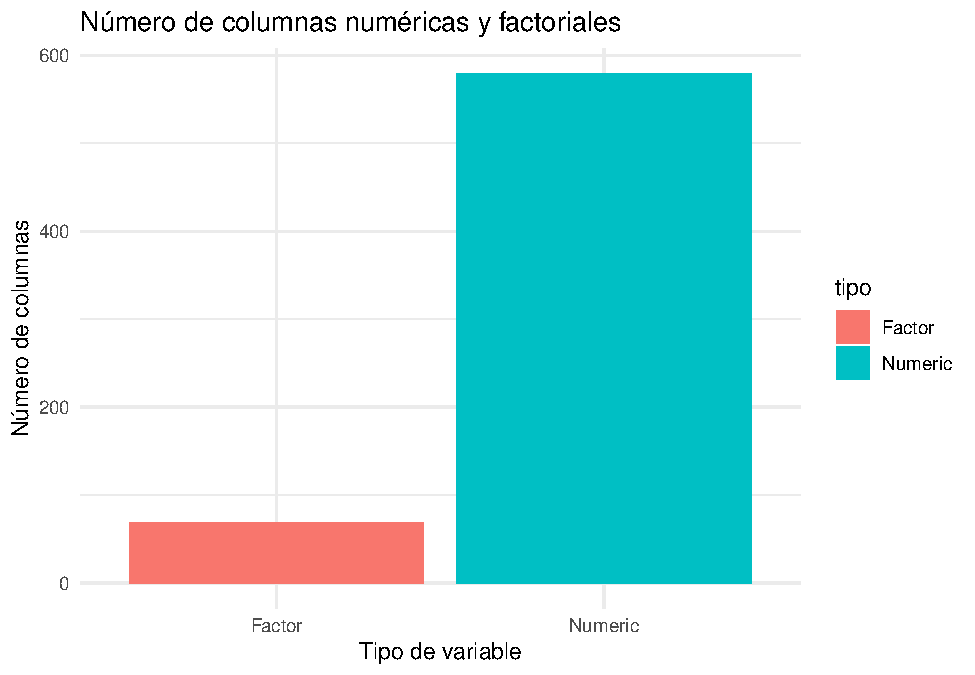
\includegraphics{./figure/unnamed-chunk-14-1} \end{center}

\begin{Shaded}
\begin{Highlighting}[]
\FunctionTok{ggplot}\NormalTok{(summary\_df, }\FunctionTok{aes}\NormalTok{(}\AttributeTok{x =}\NormalTok{ variable, }\AttributeTok{y =}\NormalTok{ tipo, }\AttributeTok{fill =}\NormalTok{ tipo)) }\SpecialCharTok{+}
  \FunctionTok{geom\_bar}\NormalTok{(}\AttributeTok{stat =} \StringTok{"identity"}\NormalTok{) }\SpecialCharTok{+}
  \FunctionTok{labs}\NormalTok{(}\AttributeTok{title =} \StringTok{"Número de columnas numéricas y factoriales"}\NormalTok{,}
       \AttributeTok{x =} \StringTok{"Tipo de variable"}\NormalTok{,}
       \AttributeTok{y =} \StringTok{"Número de columnas"}\NormalTok{) }\SpecialCharTok{+}
  \FunctionTok{theme\_minimal}\NormalTok{()}\SpecialCharTok{+}
  \FunctionTok{theme}\NormalTok{(}\AttributeTok{axis.text.x =} \FunctionTok{element\_text}\NormalTok{(}\AttributeTok{angle =} \DecValTok{90}\NormalTok{, }\AttributeTok{vjust =} \FloatTok{0.5}\NormalTok{, }\AttributeTok{hjust =} \DecValTok{1}\NormalTok{))}
\end{Highlighting}
\end{Shaded}

\begin{center}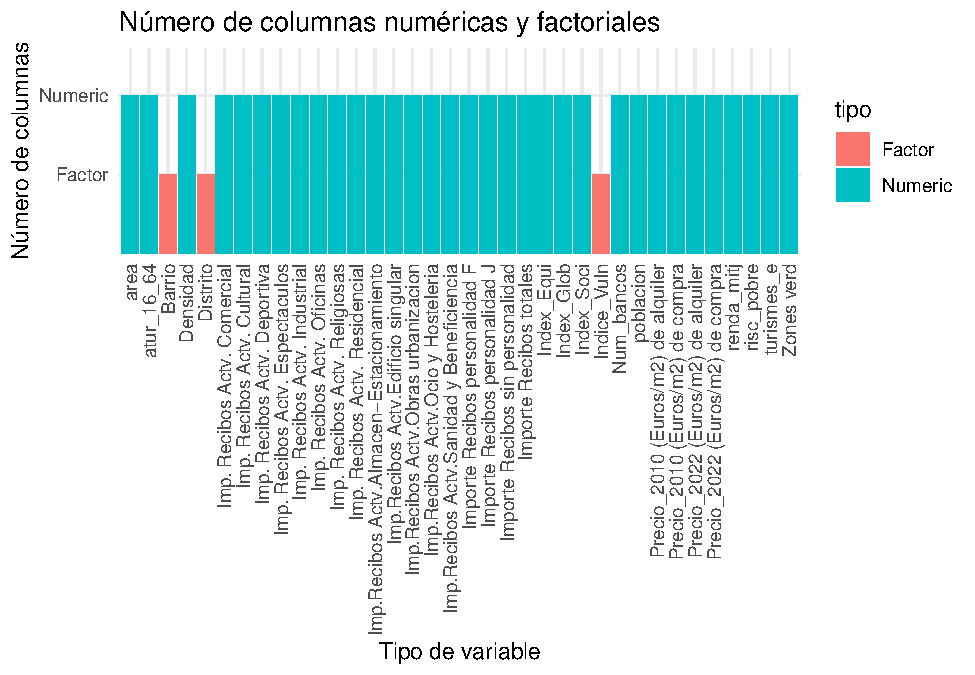
\includegraphics{./figure/unnamed-chunk-14-2} \end{center}

Tenemos un total de 33 variables numéricas (cuantitativas) y 3 variables
de tipo factor (cualitativas). Una vez creado y depurado nuestro
conjunto de forma preliminar, vamos a plantear las preguntas que
queremos resolver y acabar de poner nuestro dataset a punto.

\hypertarget{estudio-de-la-correlaciuxf3n}{%
\section{Estudio de la correlación}\label{estudio-de-la-correlaciuxf3n}}

\begin{Shaded}
\begin{Highlighting}[]
\CommentTok{\# Selecciona solo columnas numéricas}
\NormalTok{df\_numeric }\OtherTok{\textless{}{-}} \FunctionTok{select\_if}\NormalTok{(df, is.numeric)}

\CommentTok{\# Correlación de Pearson}
\NormalTok{cor\_pearson }\OtherTok{\textless{}{-}} \FunctionTok{cor}\NormalTok{(df\_numeric, }\AttributeTok{method =} \StringTok{"pearson"}\NormalTok{, }\AttributeTok{use =} \StringTok{"complete.obs"}\NormalTok{)}

\CommentTok{\# Correlación de Spearman}
\NormalTok{cor\_spearman }\OtherTok{\textless{}{-}} \FunctionTok{cor}\NormalTok{(df\_numeric, }\AttributeTok{method =} \StringTok{"spearman"}\NormalTok{, }\AttributeTok{use =} \StringTok{"complete.obs"}\NormalTok{)}
\end{Highlighting}
\end{Shaded}

\begin{Shaded}
\begin{Highlighting}[]
\CommentTok{\# Convertir la matriz de correlación a un formato largo}
\NormalTok{cor\_pearson\_long }\OtherTok{\textless{}{-}} \FunctionTok{as.data.frame}\NormalTok{(cor\_pearson) }\SpecialCharTok{\%\textgreater{}\%}
  \FunctionTok{rownames\_to\_column}\NormalTok{(}\AttributeTok{var =} \StringTok{"Variable1"}\NormalTok{) }\SpecialCharTok{\%\textgreater{}\%}
  \FunctionTok{gather}\NormalTok{(}\AttributeTok{key =} \StringTok{"Variable2"}\NormalTok{, }\AttributeTok{value =} \StringTok{"Correlation"}\NormalTok{, }\SpecialCharTok{{-}}\NormalTok{Variable1)}

\CommentTok{\# Filtrar las correlaciones mayores a 0.8 y diferentes de 1}
\NormalTok{strong\_correlations }\OtherTok{\textless{}{-}}\NormalTok{ cor\_pearson\_long }\SpecialCharTok{\%\textgreater{}\%}
  \FunctionTok{filter}\NormalTok{(}\FunctionTok{abs}\NormalTok{(Correlation) }\SpecialCharTok{\textgreater{}} \FloatTok{0.8}\NormalTok{, }\FunctionTok{abs}\NormalTok{(Correlation) }\SpecialCharTok{\textless{}} \DecValTok{1}\NormalTok{) }\SpecialCharTok{\%\textgreater{}\%}
  \FunctionTok{filter}\NormalTok{(}\SpecialCharTok{!}\FunctionTok{duplicated}\NormalTok{(}\FunctionTok{t}\NormalTok{(}\FunctionTok{apply}\NormalTok{(.[, }\FunctionTok{c}\NormalTok{(}\StringTok{"Variable1"}\NormalTok{, }\StringTok{"Variable2"}\NormalTok{)], }\DecValTok{1}\NormalTok{, sort))))}

\CommentTok{\# Mostrar los resultados}
\FunctionTok{print}\NormalTok{(strong\_correlations)}
\end{Highlighting}
\end{Shaded}

\begin{verbatim}
                                  Variable1                                Variable2 Correlation
1                                 poblacion                               atur_16_64   0.8877622
2                                Index_Soci                               renda_mitj   0.9089642
3          Precio_2022 (Euros/m2) de compra                               renda_mitj   0.9132029
4                                Index_Glob                               Index_Soci   0.9131050
5          Precio_2022 (Euros/m2) de compra                               Index_Soci   0.8495091
6  Imp.Recibos Actv.Almacen-Estacionamiento           Importe Recibos personalidad F   0.9171733
7            Imp. Recibos Actv. Residencial           Importe Recibos personalidad F   0.9974711
8                   Importe Recibos totales           Importe Recibos personalidad F   0.8846799
9              Imp. Recibos Actv. Comercial           Importe Recibos personalidad J   0.8890860
10              Imp. Recibos Actv. Oficinas           Importe Recibos personalidad J   0.8068381
11                  Importe Recibos totales           Importe Recibos personalidad J   0.8616861
12              Imp. Recibos Actv. Oficinas         Importe Recibos sin personalidad   0.8422134
13           Imp. Recibos Actv. Residencial Imp.Recibos Actv.Almacen-Estacionamiento   0.9223414
14                  Importe Recibos totales Imp.Recibos Actv.Almacen-Estacionamiento   0.9276058
15                  Importe Recibos totales             Imp. Recibos Actv. Comercial   0.8503477
16          Imp. Recibos Actv. Espectaculos              Imp. Recibos Actv. Cultural   0.8718010
17                  Importe Recibos totales           Imp. Recibos Actv. Residencial   0.8869359
\end{verbatim}

\begin{Shaded}
\begin{Highlighting}[]
\CommentTok{\# Establecer la semilla para reproducibilidad}
\FunctionTok{set.seed}\NormalTok{(}\DecValTok{130}\NormalTok{)}

\CommentTok{\# Crear un grafo}
\NormalTok{graph\_data }\OtherTok{\textless{}{-}} \FunctionTok{graph\_from\_data\_frame}\NormalTok{(strong\_correlations, }\AttributeTok{directed =} \ConstantTok{FALSE}\NormalTok{)}

\CommentTok{\# Ajustar atributos del nodo}
\FunctionTok{V}\NormalTok{(graph\_data)}\SpecialCharTok{$}\NormalTok{color }\OtherTok{\textless{}{-}} \StringTok{"skyblue"}
\FunctionTok{V}\NormalTok{(graph\_data)}\SpecialCharTok{$}\NormalTok{size }\OtherTok{\textless{}{-}} \DecValTok{6}
\FunctionTok{V}\NormalTok{(graph\_data)}\SpecialCharTok{$}\NormalTok{frame.color }\OtherTok{\textless{}{-}} \StringTok{"black"}

\CommentTok{\# Queremos que las líneas varíen entre 1 y 5 en grosor}
\NormalTok{cor\_min }\OtherTok{\textless{}{-}} \FloatTok{0.8}
\NormalTok{cor\_max }\OtherTok{\textless{}{-}} \FloatTok{1.0}
\NormalTok{width\_min }\OtherTok{\textless{}{-}} \DecValTok{1}
\NormalTok{width\_max }\OtherTok{\textless{}{-}} \DecValTok{5}
\FunctionTok{E}\NormalTok{(graph\_data)}\SpecialCharTok{$}\NormalTok{width }\OtherTok{\textless{}{-}}\NormalTok{ (}\FunctionTok{abs}\NormalTok{(}\FunctionTok{E}\NormalTok{(graph\_data)}\SpecialCharTok{$}\NormalTok{Correlation) }\SpecialCharTok{{-}}\NormalTok{ cor\_min) }\SpecialCharTok{/}\NormalTok{ (cor\_max }\SpecialCharTok{{-}}\NormalTok{ cor\_min) }\SpecialCharTok{*} 
\NormalTok{                       (width\_max }\SpecialCharTok{{-}}\NormalTok{ width\_min) }\SpecialCharTok{+}\NormalTok{ width\_min}

\CommentTok{\# Elegir un layout que ofrezca más espacio y optimizar para evitar superposición}
\NormalTok{layout }\OtherTok{\textless{}{-}} \FunctionTok{layout\_with\_fr}\NormalTok{(graph\_data)}

\CommentTok{\# Dibujar el gráfico}
\FunctionTok{par}\NormalTok{(}\AttributeTok{mar =} \FunctionTok{c}\NormalTok{(}\DecValTok{0}\NormalTok{, }\DecValTok{0}\NormalTok{, }\FloatTok{1.5}\NormalTok{, }\DecValTok{0}\NormalTok{)) }\CommentTok{\# Ajustar los márgenes si es necesario}
\FunctionTok{plot}\NormalTok{(graph\_data, }\AttributeTok{layout =}\NormalTok{ layout, }\AttributeTok{vertex.label.color =} \StringTok{"black"}\NormalTok{, }\AttributeTok{vertex.label.cex =} \FloatTok{0.7}\NormalTok{,}
     \AttributeTok{vertex.label.dist =} \FloatTok{1.2}\NormalTok{, }\CommentTok{\# Aumentar la distancia de las etiquetas de los nodos}
     \AttributeTok{edge.label =} \ConstantTok{NA}\NormalTok{, }\CommentTok{\# Ocultar las etiquetas de las aristas para despejar el gráfico}
     \AttributeTok{edge.color =} \StringTok{"gray"}\NormalTok{,}
     \AttributeTok{main =} \StringTok{"Red de Correlaciones Pearson \textgreater{} 0.8"}\NormalTok{)}
\end{Highlighting}
\end{Shaded}

\begin{center}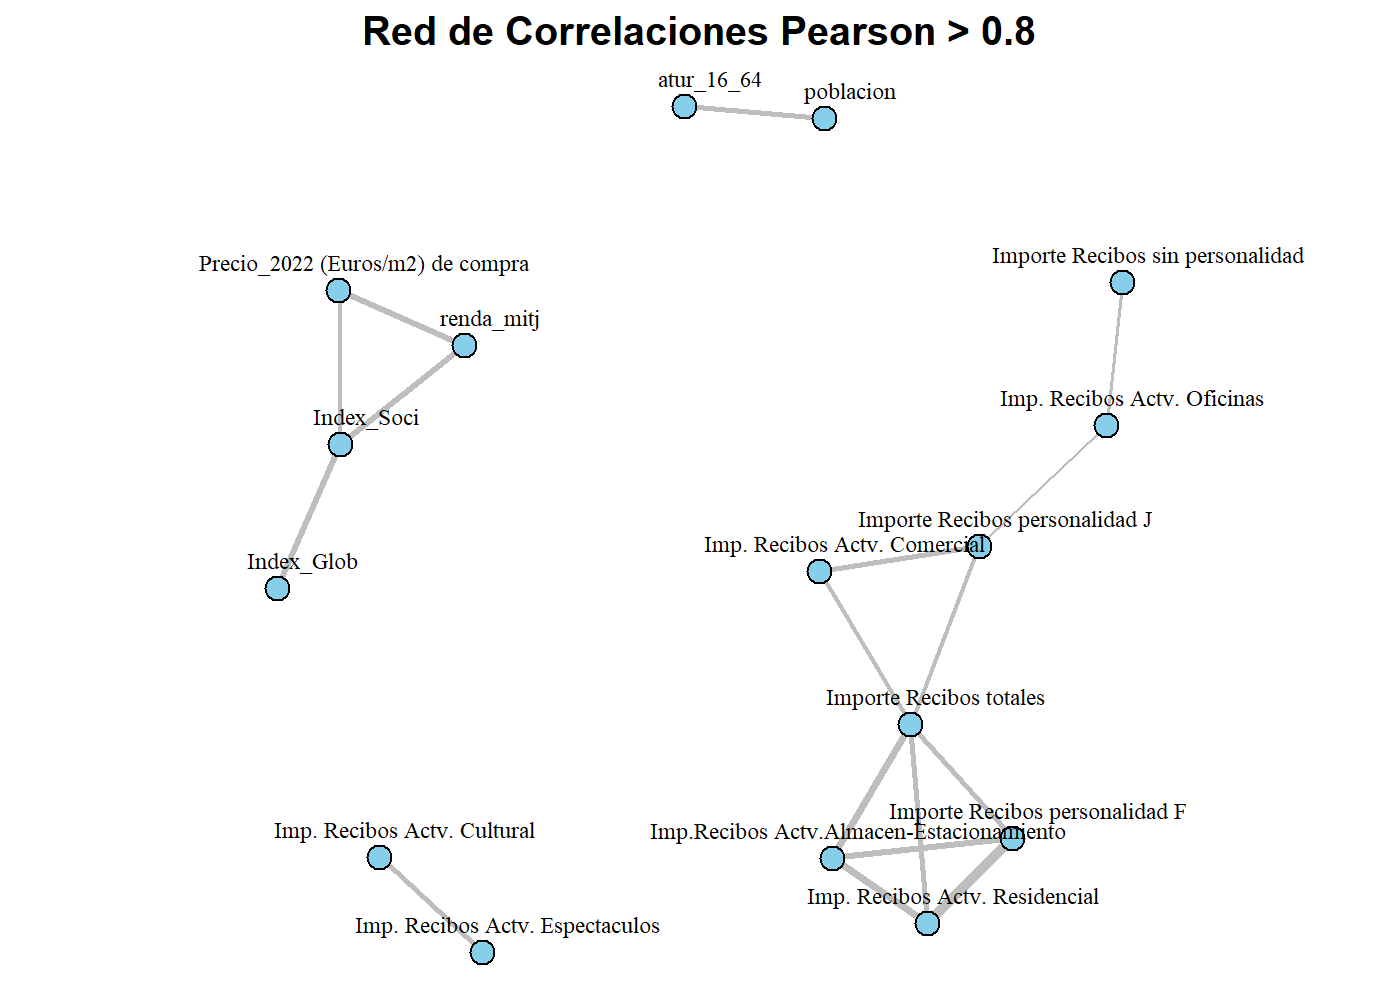
\includegraphics{./figure/unnamed-chunk-17-1} \end{center}

\begin{Shaded}
\begin{Highlighting}[]
\CommentTok{\# Crear un gráfico de etiquetas}
\FunctionTok{ggplot}\NormalTok{(strong\_correlations, }\FunctionTok{aes}\NormalTok{(}\AttributeTok{x =}\NormalTok{ Variable1, }\AttributeTok{y =}\NormalTok{ Variable2, }\AttributeTok{label =} \FunctionTok{round}\NormalTok{(Correlation, }\DecValTok{2}\NormalTok{))) }\SpecialCharTok{+}
  \FunctionTok{geom\_tile}\NormalTok{(}\FunctionTok{aes}\NormalTok{(}\AttributeTok{fill =}\NormalTok{ Correlation), }\AttributeTok{color =} \StringTok{"white"}\NormalTok{) }\SpecialCharTok{+}
  \FunctionTok{geom\_text}\NormalTok{() }\SpecialCharTok{+}
  \FunctionTok{scale\_fill\_gradient2}\NormalTok{(}\AttributeTok{low =} \StringTok{"blue"}\NormalTok{, }\AttributeTok{high =} \StringTok{"red"}\NormalTok{, }\AttributeTok{mid =} \StringTok{"white"}\NormalTok{, }\AttributeTok{midpoint =} \FloatTok{0.8}\NormalTok{) }\SpecialCharTok{+}
  \FunctionTok{theme\_minimal}\NormalTok{() }\SpecialCharTok{+}
  \FunctionTok{theme}\NormalTok{(}\AttributeTok{axis.text.x =} \FunctionTok{element\_text}\NormalTok{(}\AttributeTok{angle =} \DecValTok{45}\NormalTok{, }\AttributeTok{hjust =} \DecValTok{1}\NormalTok{))}
\end{Highlighting}
\end{Shaded}

\begin{center}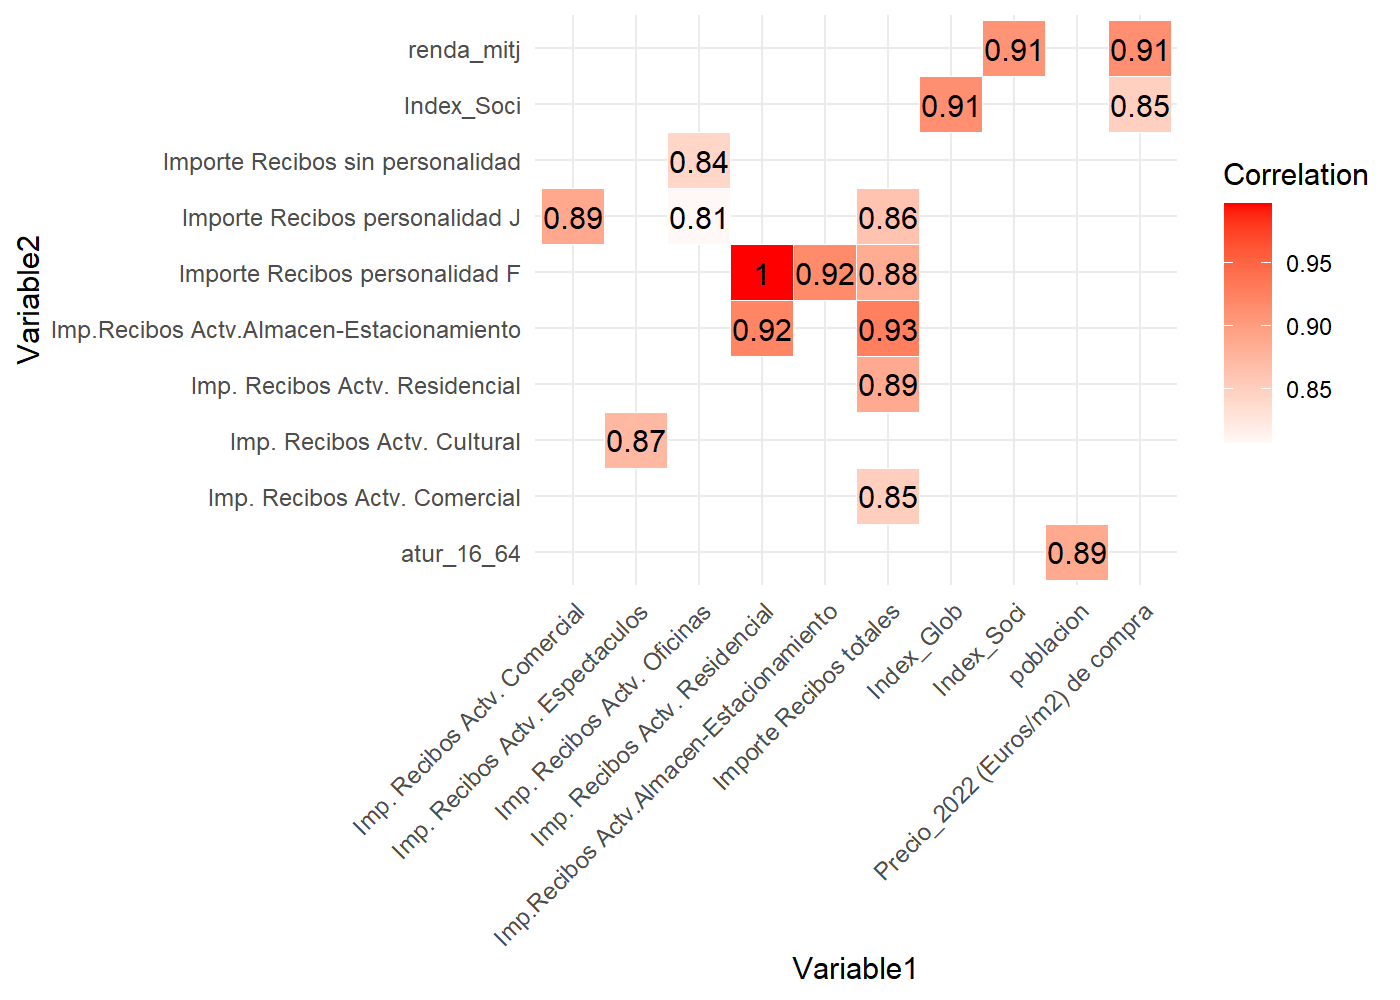
\includegraphics{./figure/unnamed-chunk-18-1} \end{center}

\begin{Shaded}
\begin{Highlighting}[]
\CommentTok{\# Convertir cor\_pearson a formato largo}
\NormalTok{cor\_pearson\_long }\OtherTok{\textless{}{-}}\NormalTok{ cor\_pearson }\SpecialCharTok{\%\textgreater{}\%} 
                    \FunctionTok{as.data.frame}\NormalTok{() }\SpecialCharTok{\%\textgreater{}\%} 
                    \FunctionTok{rownames\_to\_column}\NormalTok{(}\AttributeTok{var =} \StringTok{"Variable1"}\NormalTok{) }\SpecialCharTok{\%\textgreater{}\%} 
                    \FunctionTok{gather}\NormalTok{(}\AttributeTok{key =} \StringTok{"Variable2"}\NormalTok{, }\AttributeTok{value =} \StringTok{"Correlation"}\NormalTok{, }\SpecialCharTok{{-}}\NormalTok{Variable1)}

\CommentTok{\# Visualizar con ggplot2}
\FunctionTok{ggplot}\NormalTok{(cor\_pearson\_long, }\FunctionTok{aes}\NormalTok{(}\AttributeTok{x =}\NormalTok{ Variable1, }\AttributeTok{y =}\NormalTok{ Variable2, }\AttributeTok{fill =}\NormalTok{ Correlation)) }\SpecialCharTok{+}
    \FunctionTok{geom\_tile}\NormalTok{() }\SpecialCharTok{+}
    \FunctionTok{scale\_fill\_gradient2}\NormalTok{(}\AttributeTok{low =} \StringTok{"blue"}\NormalTok{, }\AttributeTok{high =} \StringTok{"red"}\NormalTok{, }\AttributeTok{mid =} \StringTok{"white"}\NormalTok{, }\AttributeTok{midpoint =} \DecValTok{0}\NormalTok{) }\SpecialCharTok{+}
    \FunctionTok{theme\_minimal}\NormalTok{() }\SpecialCharTok{+}
    \FunctionTok{theme}\NormalTok{(}\AttributeTok{axis.text.x =} \FunctionTok{element\_text}\NormalTok{(}\AttributeTok{angle =} \DecValTok{45}\NormalTok{, }\AttributeTok{hjust =} \DecValTok{1}\NormalTok{))}
\end{Highlighting}
\end{Shaded}

\begin{center}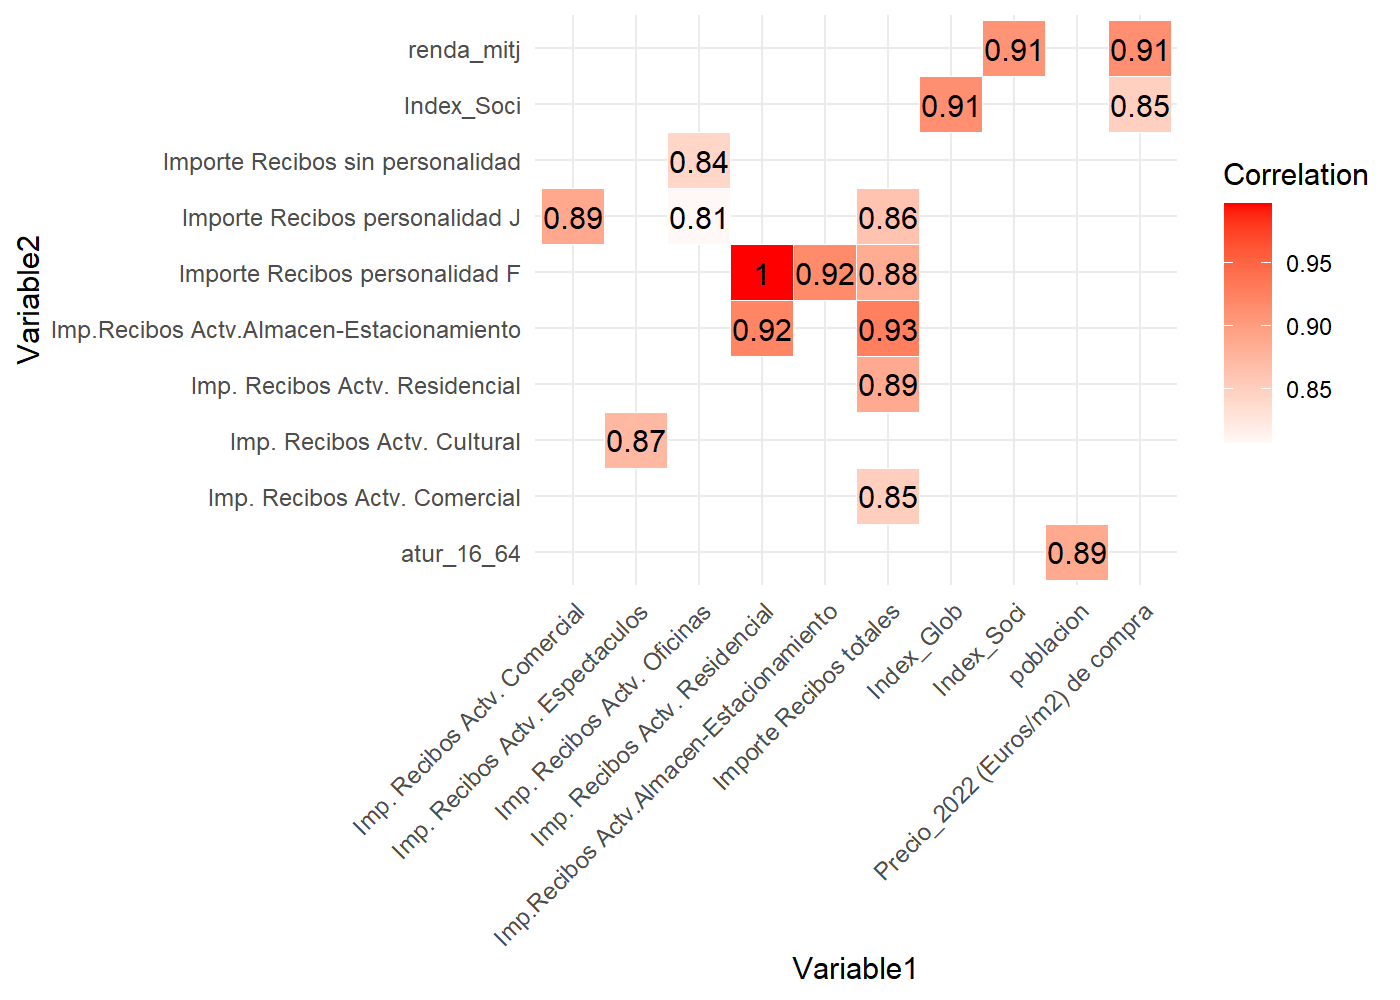
\includegraphics{./figure/unnamed-chunk-19-1} \end{center}

\begin{Shaded}
\begin{Highlighting}[]
\CommentTok{\# Suponiendo que tu dataframe se llama df}
\FunctionTok{write.table}\NormalTok{(df, }\AttributeTok{file =} \StringTok{"barrios.txt"}\NormalTok{, }\AttributeTok{sep =} \StringTok{"}\SpecialCharTok{\textbackslash{}t}\StringTok{"}\NormalTok{)}
\end{Highlighting}
\end{Shaded}

\hypertarget{estudio-de-la-vulnerabilidad}{%
\section{Estudio de la
vulnerabilidad}\label{estudio-de-la-vulnerabilidad}}

\hypertarget{mapa-de-barrios-vulnerables}{%
\subsection{Mapa de barrios
vulnerables}\label{mapa-de-barrios-vulnerables}}

\begin{Shaded}
\begin{Highlighting}[]
\CommentTok{\#primero creamos un mapa con los barrios y distrito}

\CommentTok{\# Lee el archivo GeoJSON}
\NormalTok{datos\_geojson }\OtherTok{\textless{}{-}} \FunctionTok{st\_read}\NormalTok{(}\StringTok{"./data/barris{-}barrios.geojson"}\NormalTok{)}
\end{Highlighting}
\end{Shaded}

\begin{verbatim}
Reading layer `barris-barrios' from data source 
  `C:\Users\mateo\OneDrive\Escritorio\Archivos uni\Master\Exploratorio\Proyecto\ProyectoAED2023\ProyectoAED2023\data\barris-barrios.geojson' 
  using driver `GeoJSON'
Simple feature collection with 88 features and 6 fields
Geometry type: POLYGON
Dimension:     XY
Bounding box:  xmin: -0.432535 ymin: 39.27893 xmax: -0.2753685 ymax: 39.56659
Geodetic CRS:  WGS 84
\end{verbatim}

\begin{Shaded}
\begin{Highlighting}[]
\CommentTok{\#datos\_geojson$nombre[datos\_geojson$nombre \%in\% df$Barrio]}
\CommentTok{\#df$Barrio[!df$Barrio \%in\% datos\_geojson$nombre]}
\end{Highlighting}
\end{Shaded}

\begin{Shaded}
\begin{Highlighting}[]
\CommentTok{\# Añado la columna Indice\_Vuln al dataframe desde el cual hago el mapa}
\NormalTok{vuln2 }\OtherTok{\textless{}{-}}\NormalTok{ vuln[}\FunctionTok{c}\NormalTok{(}\StringTok{\textquotesingle{}Barrio\textquotesingle{}}\NormalTok{,}\StringTok{\textquotesingle{}Indice\_Vuln\textquotesingle{}}\NormalTok{)]}
\FunctionTok{colnames}\NormalTok{(vuln2) }\OtherTok{\textless{}{-}} \FunctionTok{c}\NormalTok{(}\StringTok{\textquotesingle{}nombre\textquotesingle{}}\NormalTok{,}\StringTok{\textquotesingle{}Indice\_Vuln\textquotesingle{}}\NormalTok{)}
\NormalTok{datos\_geojson }\OtherTok{\textless{}{-}} \FunctionTok{merge}\NormalTok{(}\AttributeTok{x =}\NormalTok{ datos\_geojson, }\AttributeTok{y =}\NormalTok{ vuln2)}

\CommentTok{\# Creo los popup del mapa}
\NormalTok{popups }\OtherTok{\textless{}{-}} \FunctionTok{paste0}\NormalTok{(}\StringTok{"\textless{}b\textgreater{}"}\NormalTok{, datos\_geojson}\SpecialCharTok{$}\NormalTok{nombre, }\StringTok{"\textless{}/b\textgreater{}"}\NormalTok{, }\StringTok{"\textless{}hr\textgreater{}"}\NormalTok{, datos\_geojson}\SpecialCharTok{$}\NormalTok{Indice\_Vuln)}

\CommentTok{\# Escojo una paleta de colores}
\NormalTok{pal }\OtherTok{\textless{}{-}} \FunctionTok{colorFactor}\NormalTok{(}\FunctionTok{c}\NormalTok{(}\StringTok{\textquotesingle{}red\textquotesingle{}}\NormalTok{,}\StringTok{\textquotesingle{}gray\textquotesingle{}}\NormalTok{,}\StringTok{\textquotesingle{}blue\textquotesingle{}}\NormalTok{,}\StringTok{\textquotesingle{}green\textquotesingle{}}\NormalTok{), }\AttributeTok{levels =} \FunctionTok{levels}\NormalTok{(datos\_geojson}\SpecialCharTok{$}\NormalTok{Indice\_Vuln))}

\CommentTok{\# Creo el mapa}
\FunctionTok{leaflet}\NormalTok{(}\AttributeTok{data =}\NormalTok{ datos\_geojson) }\SpecialCharTok{\%\textgreater{}\%}
  \FunctionTok{addTiles}\NormalTok{() }\SpecialCharTok{\%\textgreater{}\%}
  \FunctionTok{addPolygons}\NormalTok{(}\AttributeTok{fillColor =} \FunctionTok{pal}\NormalTok{(datos\_geojson}\SpecialCharTok{$}\NormalTok{Indice\_Vuln),}
              \AttributeTok{weight =} \DecValTok{1}\NormalTok{,}
              \AttributeTok{opacity =} \DecValTok{1}\NormalTok{,}
              \AttributeTok{highlightOptions =} \FunctionTok{highlightOptions}\NormalTok{(}\AttributeTok{color =} \StringTok{"white"}\NormalTok{,}
                                                  \AttributeTok{weight =} \DecValTok{2}\NormalTok{,}
                                                  \AttributeTok{bringToFront =} \ConstantTok{TRUE}\NormalTok{),}
              \AttributeTok{color =} \StringTok{\textquotesingle{}black\textquotesingle{}}\NormalTok{,}
              \AttributeTok{fillOpacity =} \FloatTok{0.8}\NormalTok{,}
              \AttributeTok{popup =}\NormalTok{ popups) }\SpecialCharTok{\%\textgreater{}\%}
  \FunctionTok{addLegend}\NormalTok{(}\AttributeTok{data =}\NormalTok{ datos\_geojson,}
            \AttributeTok{position =} \StringTok{\textquotesingle{}bottomright\textquotesingle{}}\NormalTok{,}
            \AttributeTok{pal =}\NormalTok{ pal, }\AttributeTok{values =} \SpecialCharTok{\textasciitilde{}}\NormalTok{Indice\_Vuln,}
            \AttributeTok{title =} \StringTok{\textquotesingle{}Leyenda\textquotesingle{}}\NormalTok{,}
            \AttributeTok{opacity =} \DecValTok{1}\NormalTok{)}
\end{Highlighting}
\end{Shaded}

\begin{center}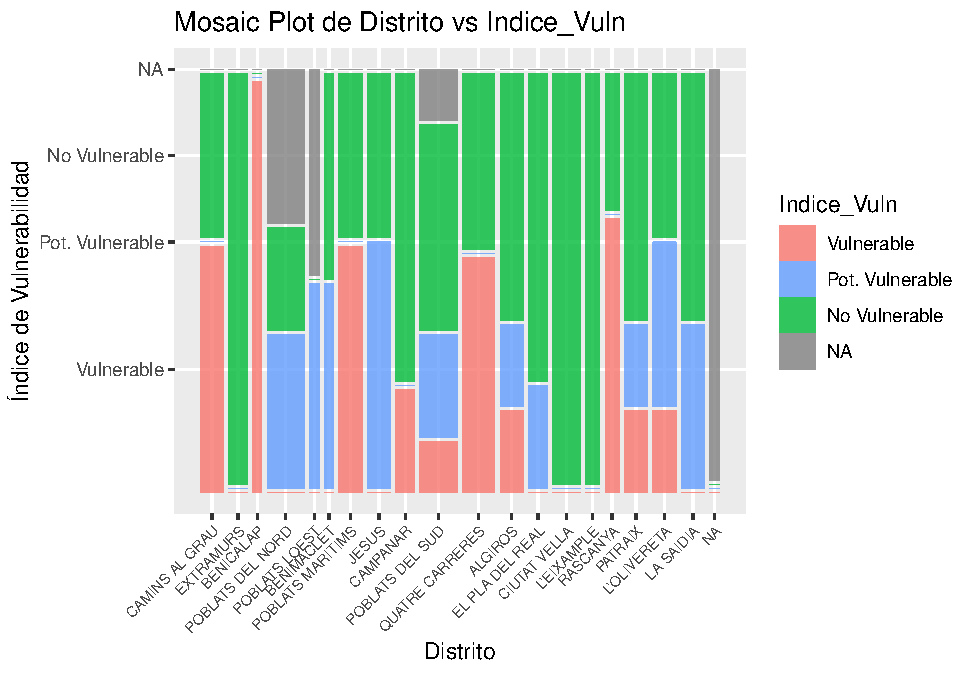
\includegraphics{./figure/unnamed-chunk-22-1} \end{center}

\hypertarget{representaciuxf3n-de-los-datos}{%
\subsection{Representación de los
datos}\label{representaciuxf3n-de-los-datos}}

\begin{Shaded}
\begin{Highlighting}[]
\CommentTok{\# me quedo con las columnas numéricas + Indice\_Vuln de df}
\NormalTok{columnas\_numericas }\OtherTok{\textless{}{-}}\NormalTok{ df }\SpecialCharTok{\%\textgreater{}\%}
  \FunctionTok{select\_if}\NormalTok{(is.numeric) }\SpecialCharTok{\%\textgreater{}\%}
  \FunctionTok{colnames}\NormalTok{()}
\NormalTok{columnas\_numéricas }\OtherTok{\textless{}{-}} \FunctionTok{c}\NormalTok{(columnas\_numericas, }\StringTok{\textquotesingle{}Indice\_Vuln\textquotesingle{}}\NormalTok{)}
\NormalTok{columnas\_numéricas }\OtherTok{\textless{}{-}}\NormalTok{ df[columnas\_numéricas]}

\CommentTok{\# Muestro un box{-}plot para cada variable numérica diferenciando 4 distribuciones en función de la vulnerabilidad}
\ControlFlowTok{for}\NormalTok{ (i }\ControlFlowTok{in}\NormalTok{ columnas\_numericas) \{}
\NormalTok{  p}\OtherTok{\textless{}{-}}\FunctionTok{ggplot}\NormalTok{(columnas\_numéricas, }\FunctionTok{aes}\NormalTok{(}\AttributeTok{x =}\NormalTok{ Indice\_Vuln, }\AttributeTok{y =}\NormalTok{.data[[i]])) }\SpecialCharTok{+}
    \FunctionTok{geom\_boxplot}\NormalTok{() }\SpecialCharTok{+} 
    \FunctionTok{ggtitle}\NormalTok{(}\FunctionTok{paste}\NormalTok{(}\StringTok{"Relación "}\NormalTok{, i))}
  \FunctionTok{print}\NormalTok{(p)}
\NormalTok{\}}
\end{Highlighting}
\end{Shaded}

\begin{center}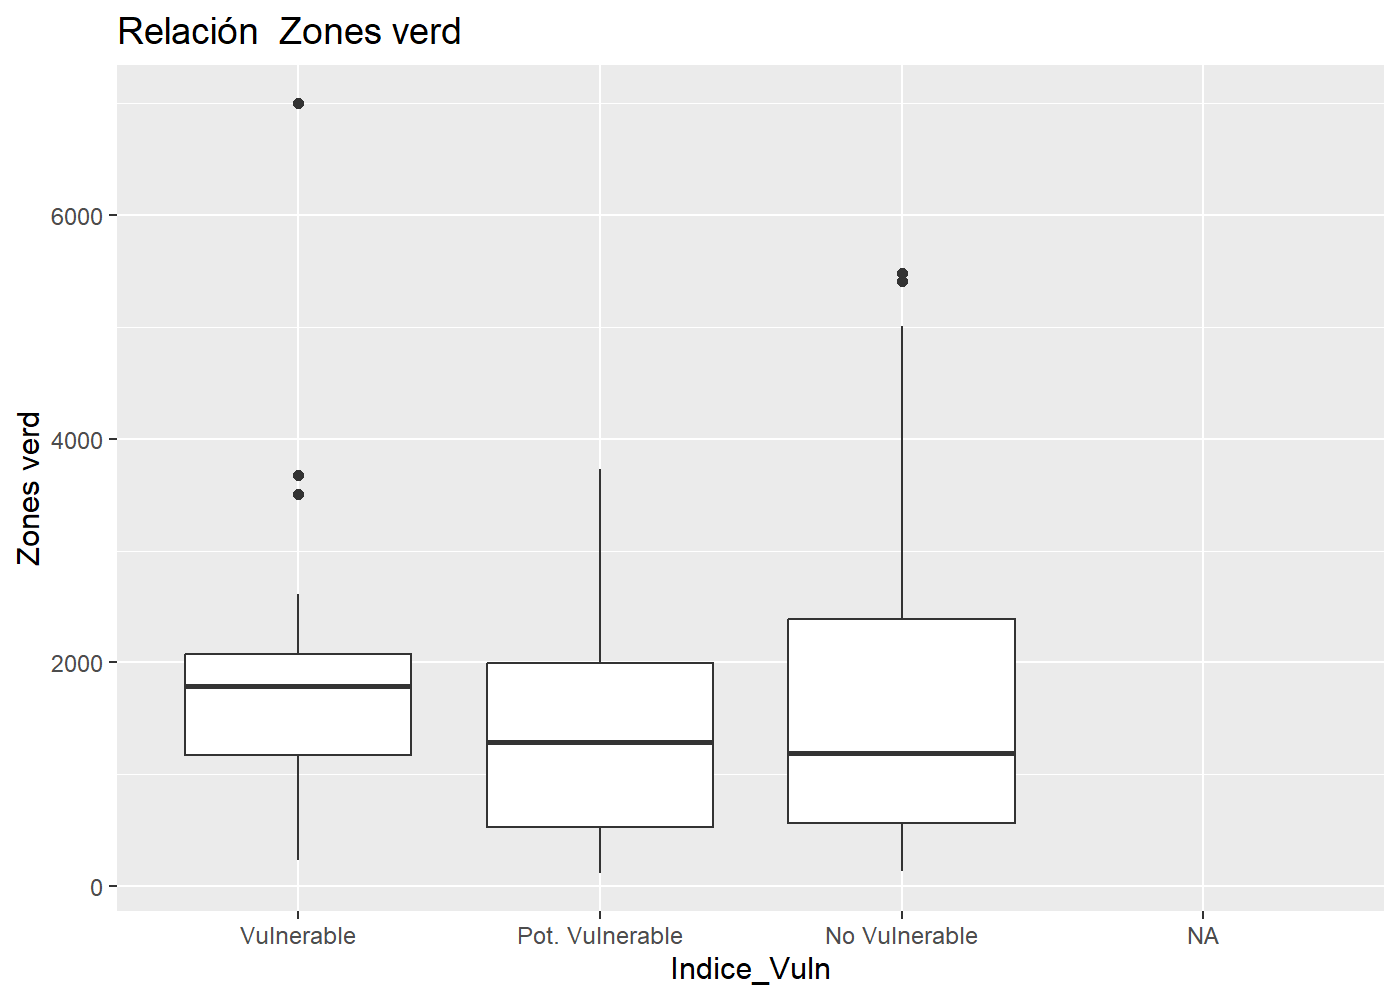
\includegraphics{./figure/unnamed-chunk-23-1} \end{center}

\begin{center}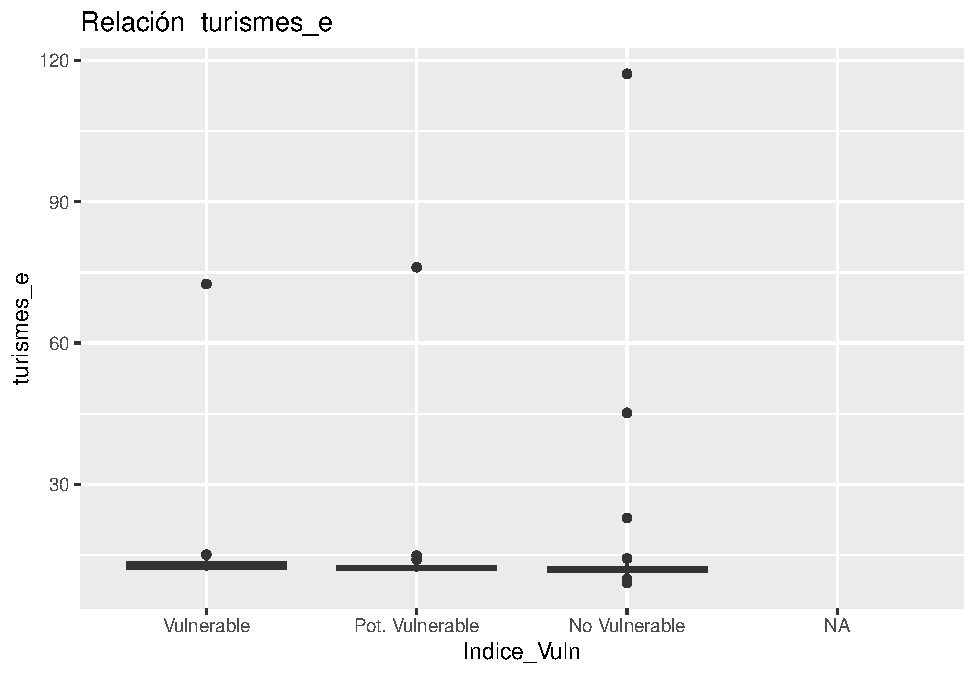
\includegraphics{./figure/unnamed-chunk-23-2} \end{center}

\begin{center}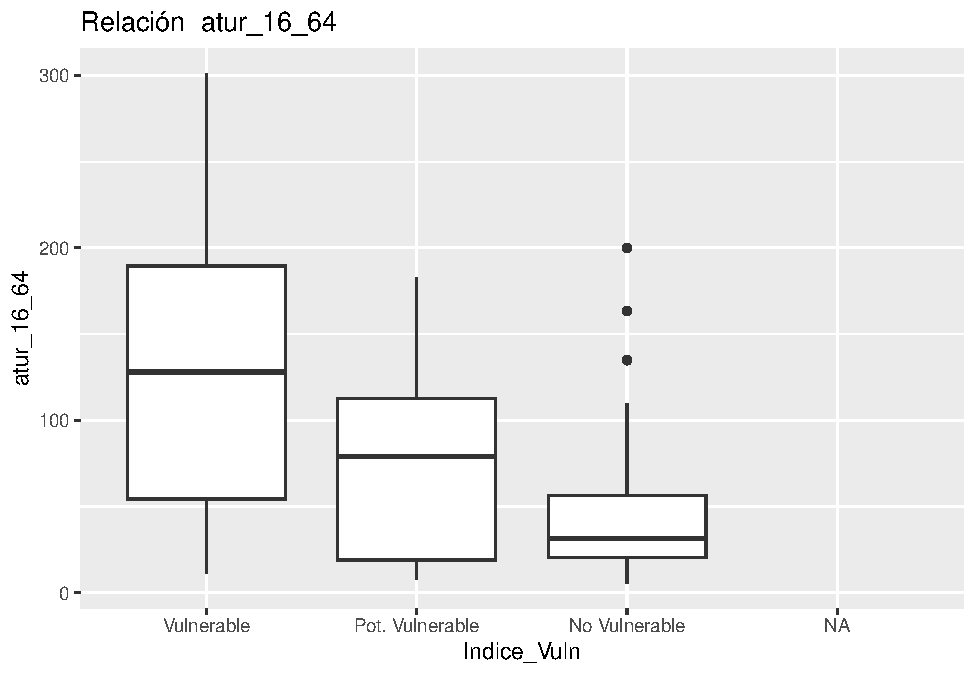
\includegraphics{./figure/unnamed-chunk-23-3} \end{center}

\begin{center}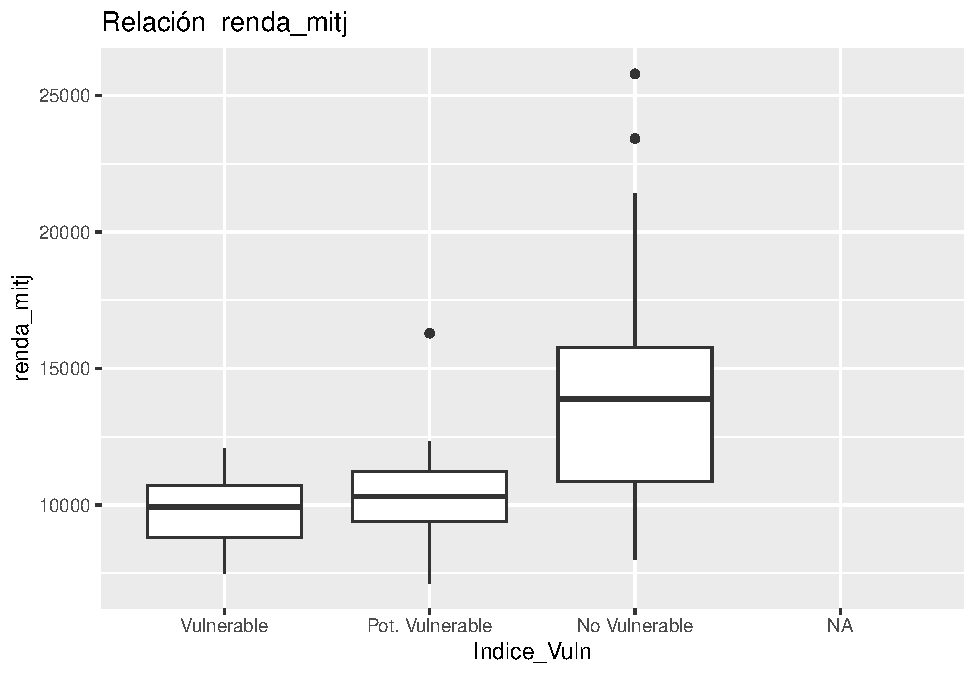
\includegraphics{./figure/unnamed-chunk-23-4} \end{center}

\begin{center}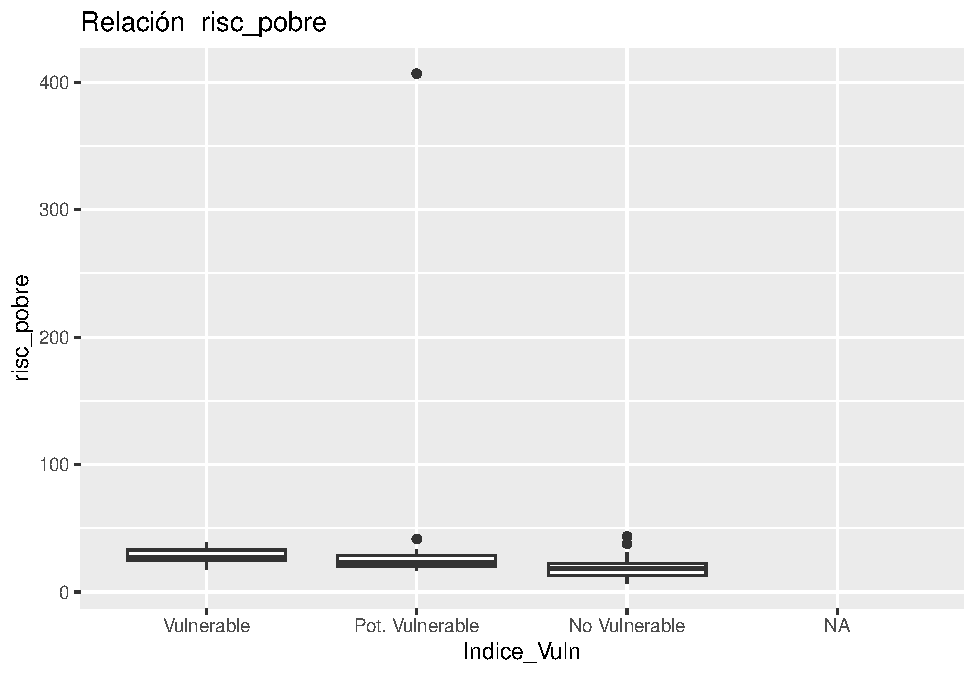
\includegraphics{./figure/unnamed-chunk-23-5} \end{center}

\begin{center}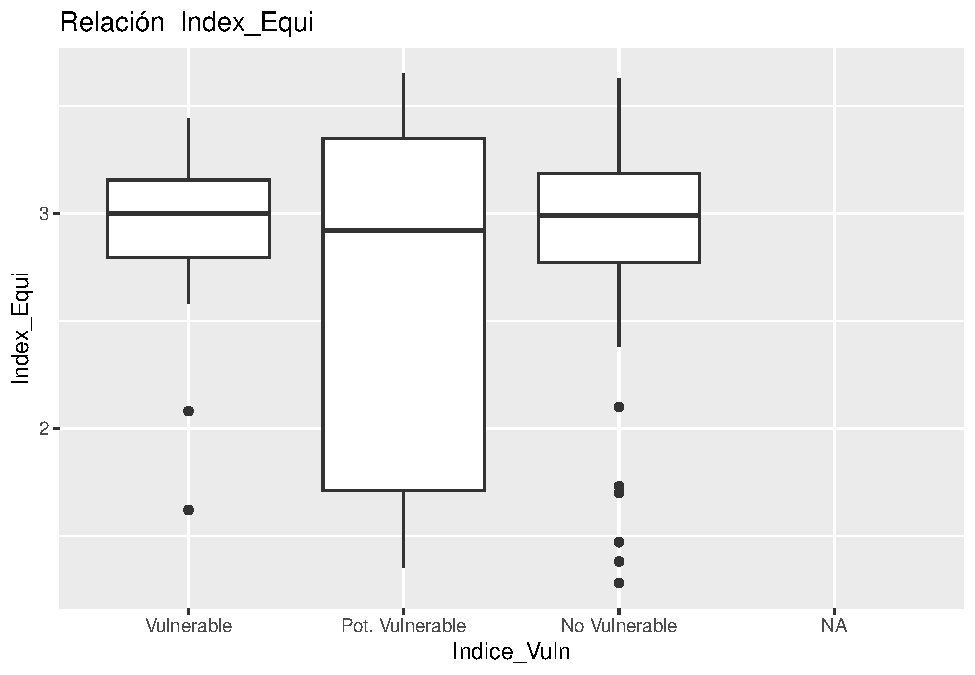
\includegraphics{./figure/unnamed-chunk-23-6} \end{center}

\begin{center}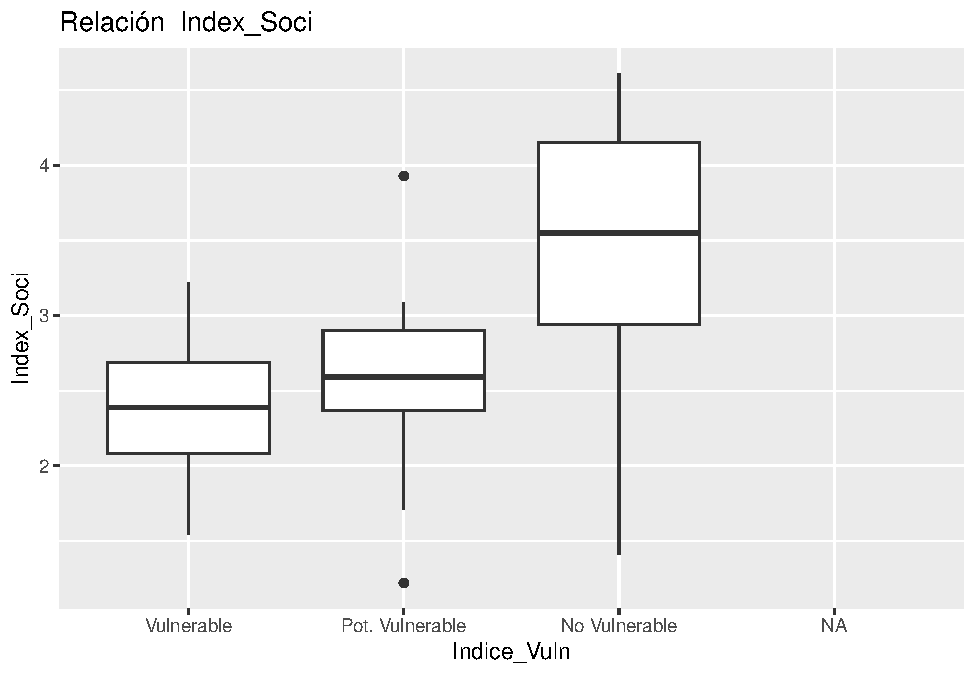
\includegraphics{./figure/unnamed-chunk-23-7} \end{center}

\begin{center}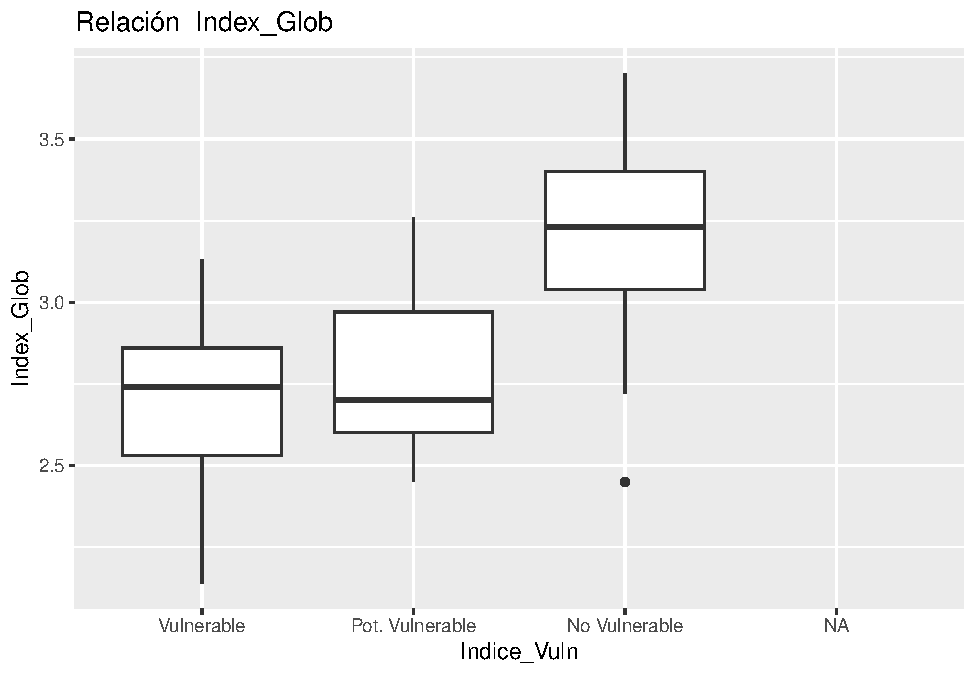
\includegraphics{./figure/unnamed-chunk-23-8} \end{center}

\begin{center}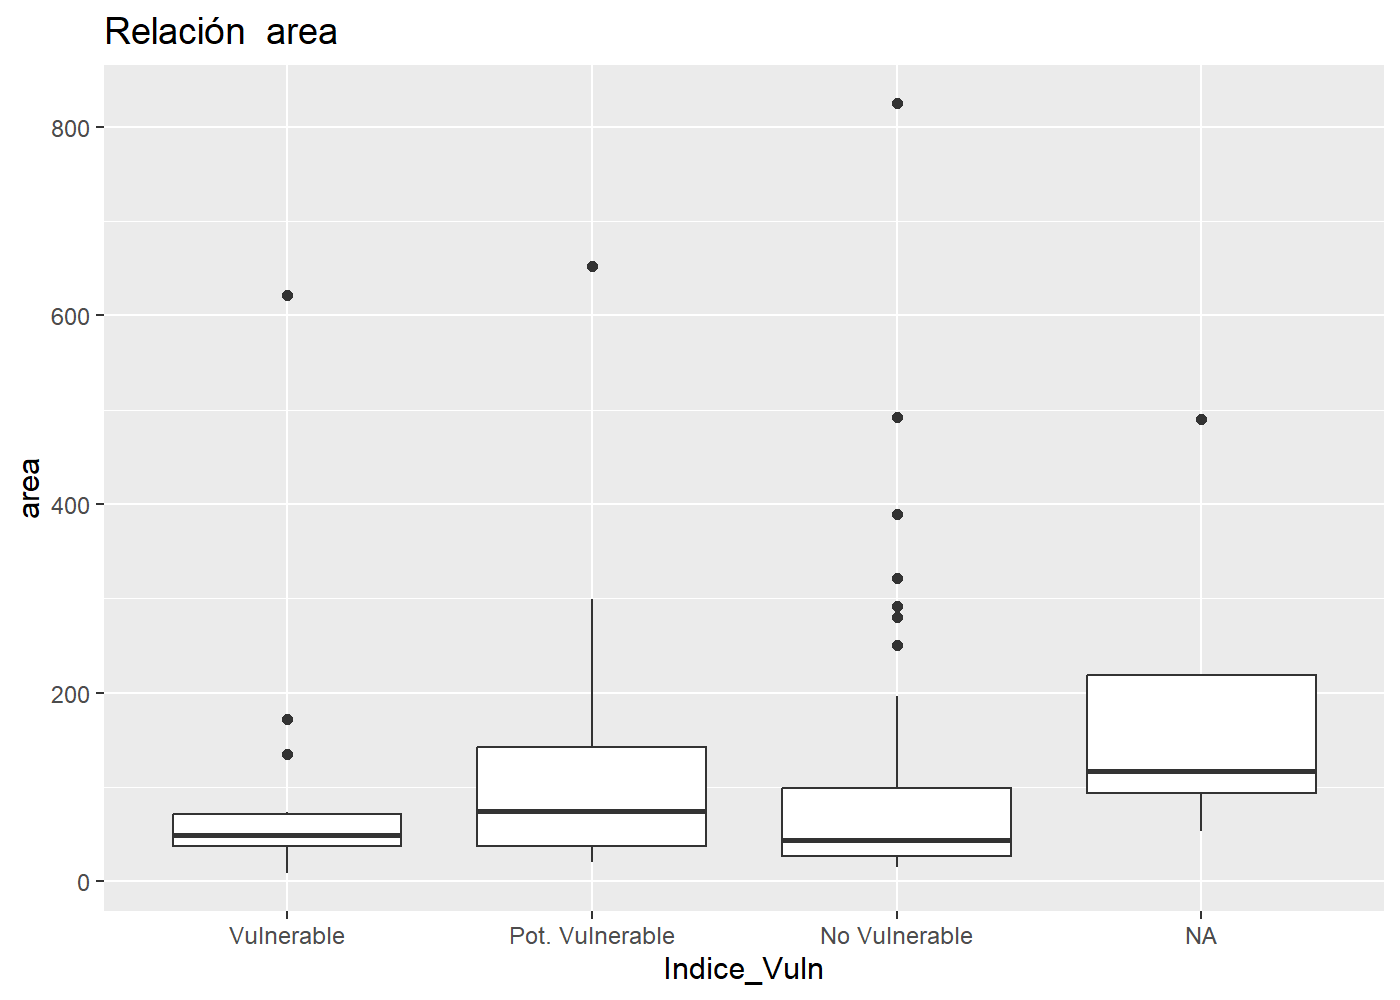
\includegraphics{./figure/unnamed-chunk-23-9} \end{center}

\begin{center}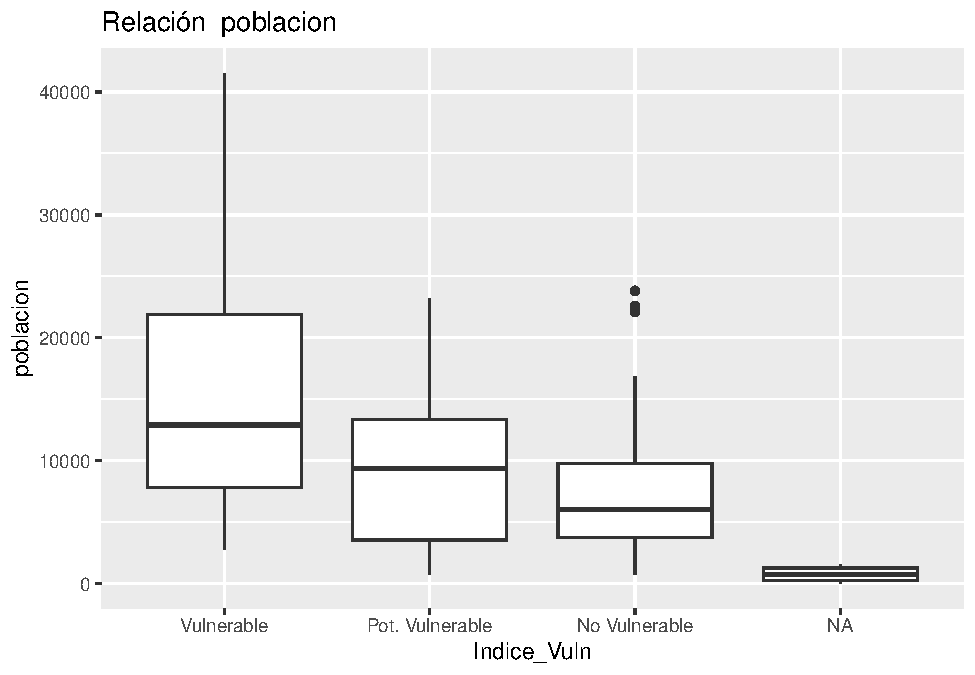
\includegraphics{./figure/unnamed-chunk-23-10} \end{center}

\begin{center}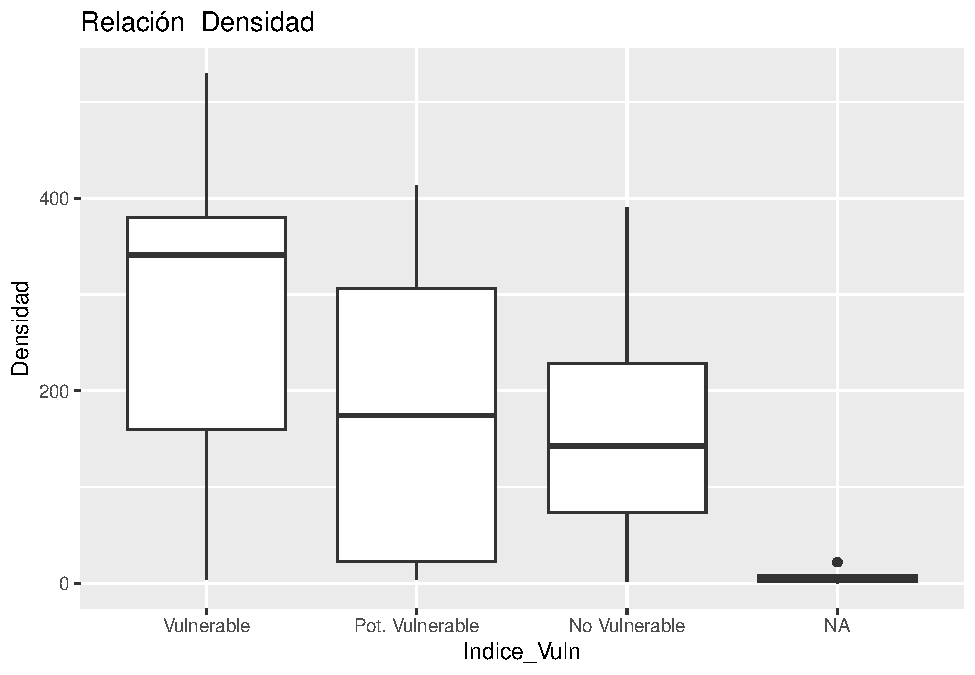
\includegraphics{./figure/unnamed-chunk-23-11} \end{center}

\begin{center}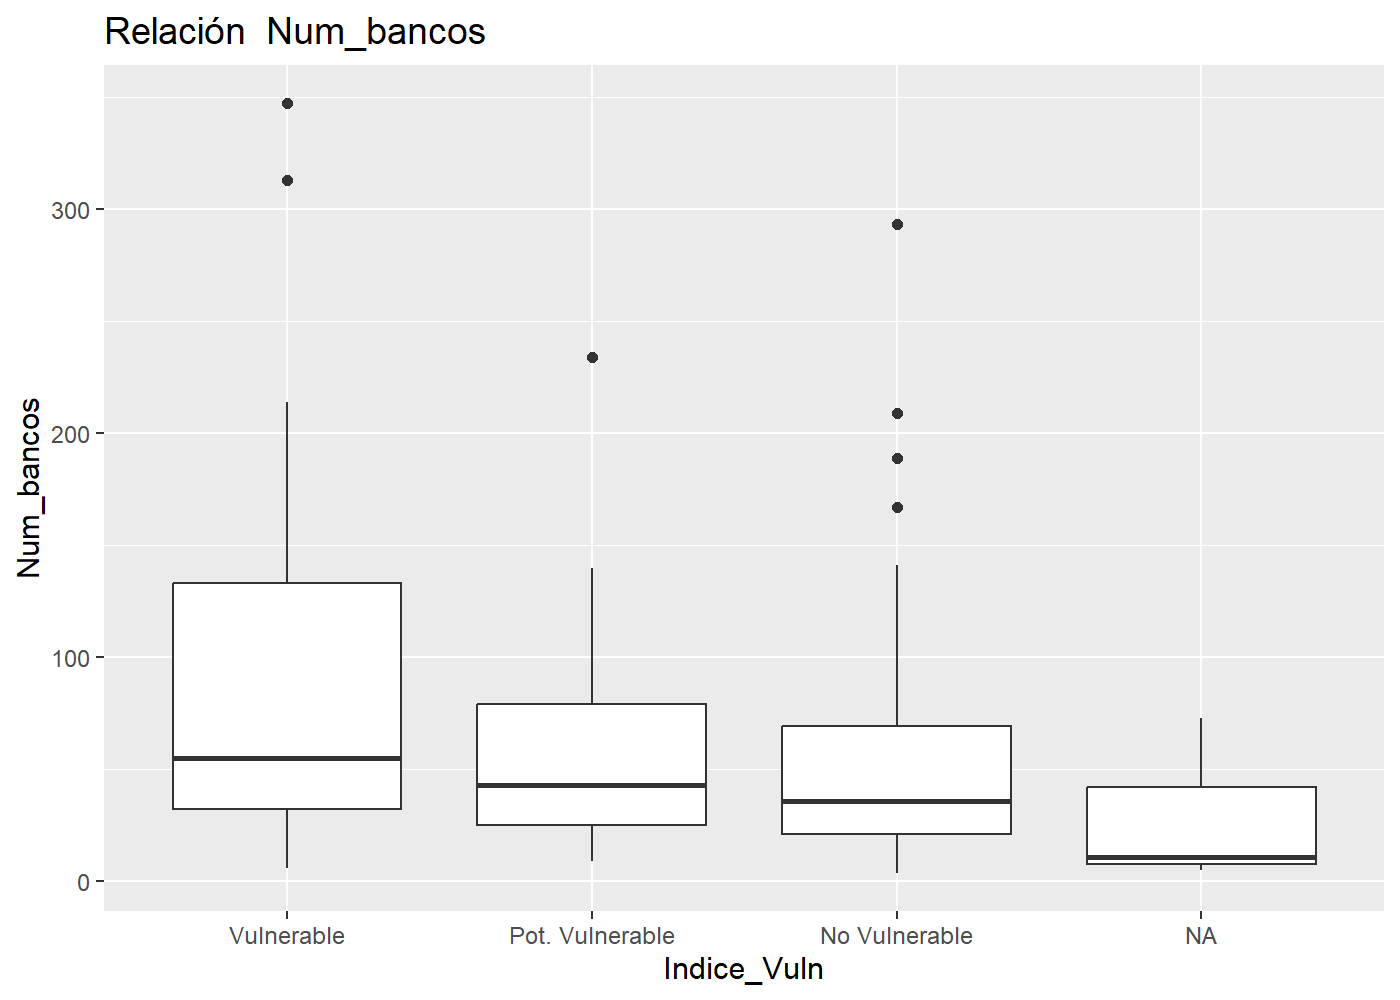
\includegraphics{./figure/unnamed-chunk-23-12} \end{center}

\begin{center}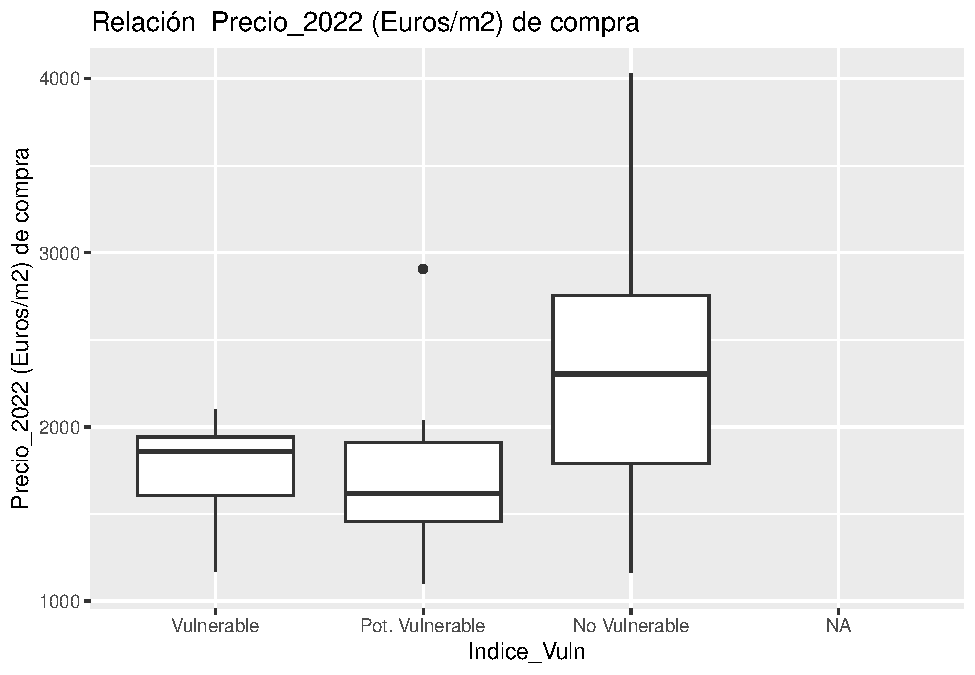
\includegraphics{./figure/unnamed-chunk-23-13} \end{center}

\begin{center}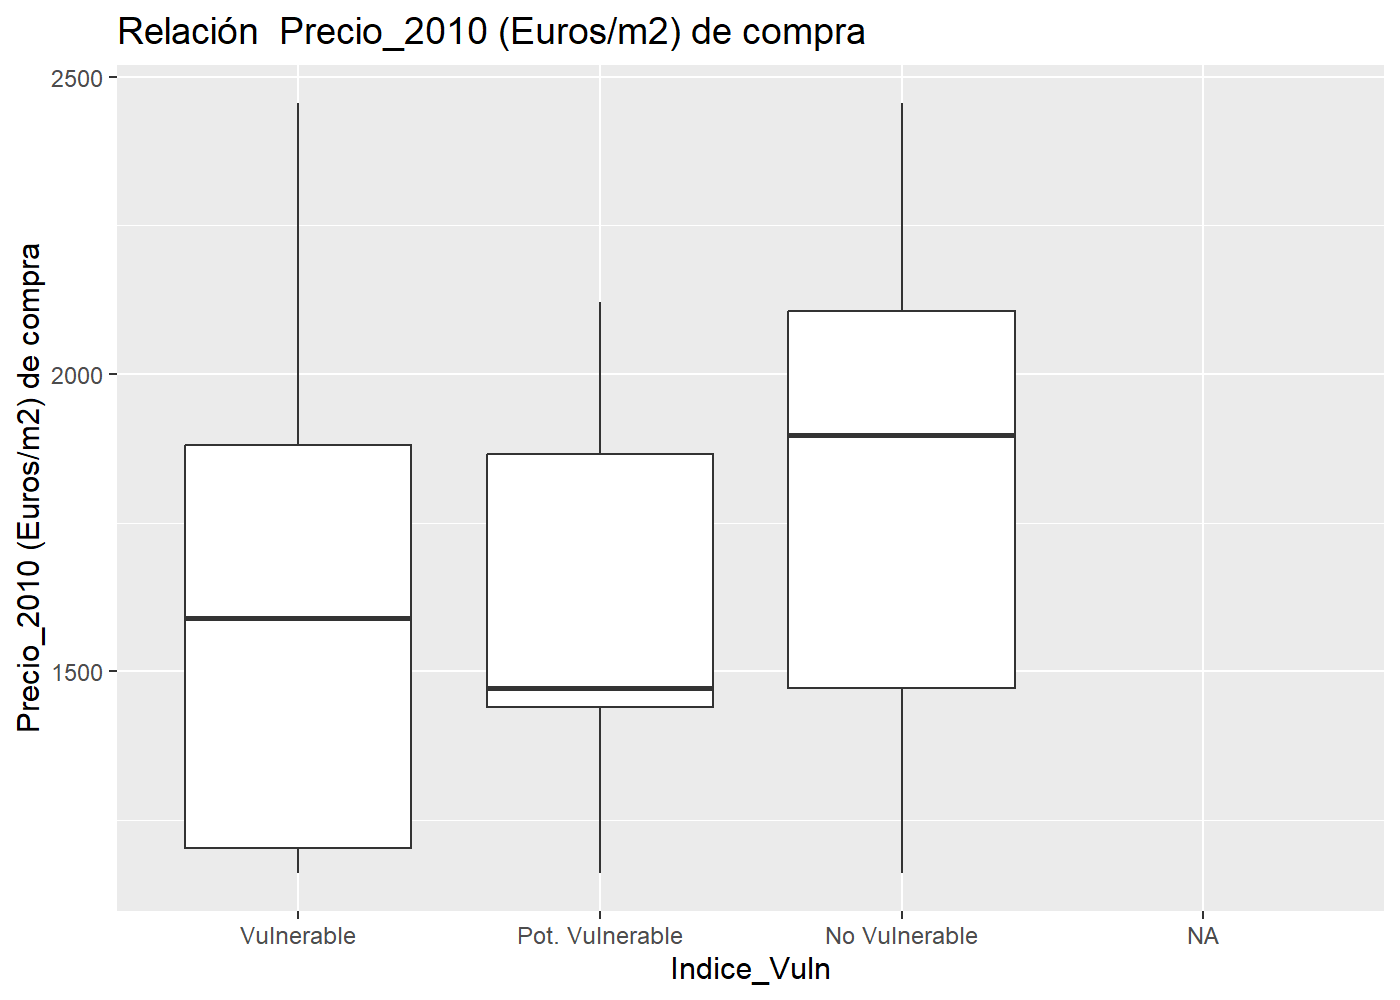
\includegraphics{./figure/unnamed-chunk-23-14} \end{center}

\begin{center}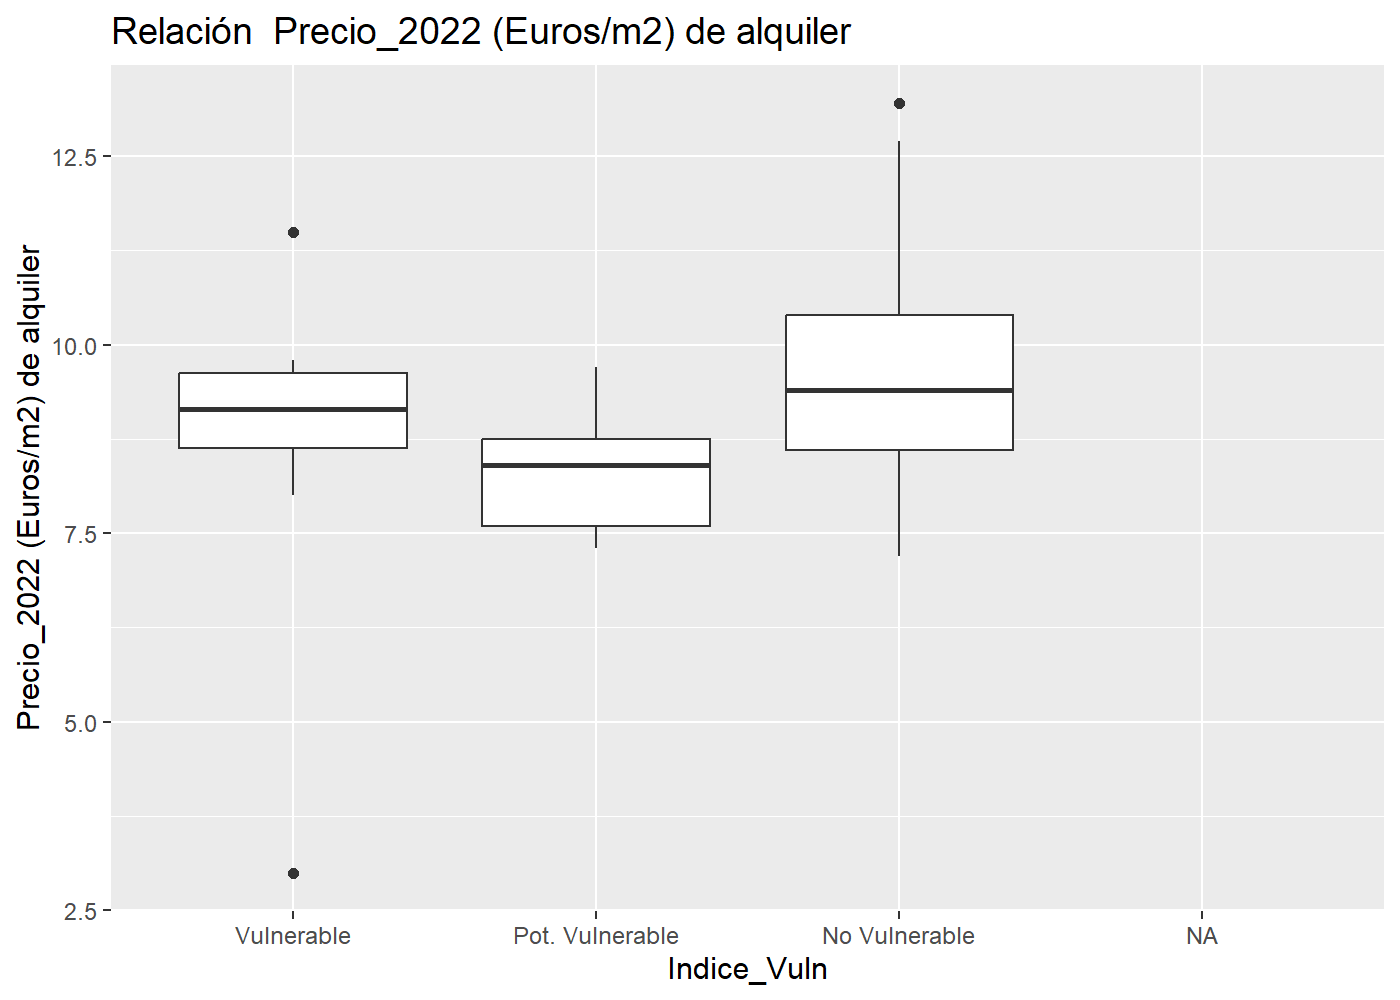
\includegraphics{./figure/unnamed-chunk-23-15} \end{center}

\begin{center}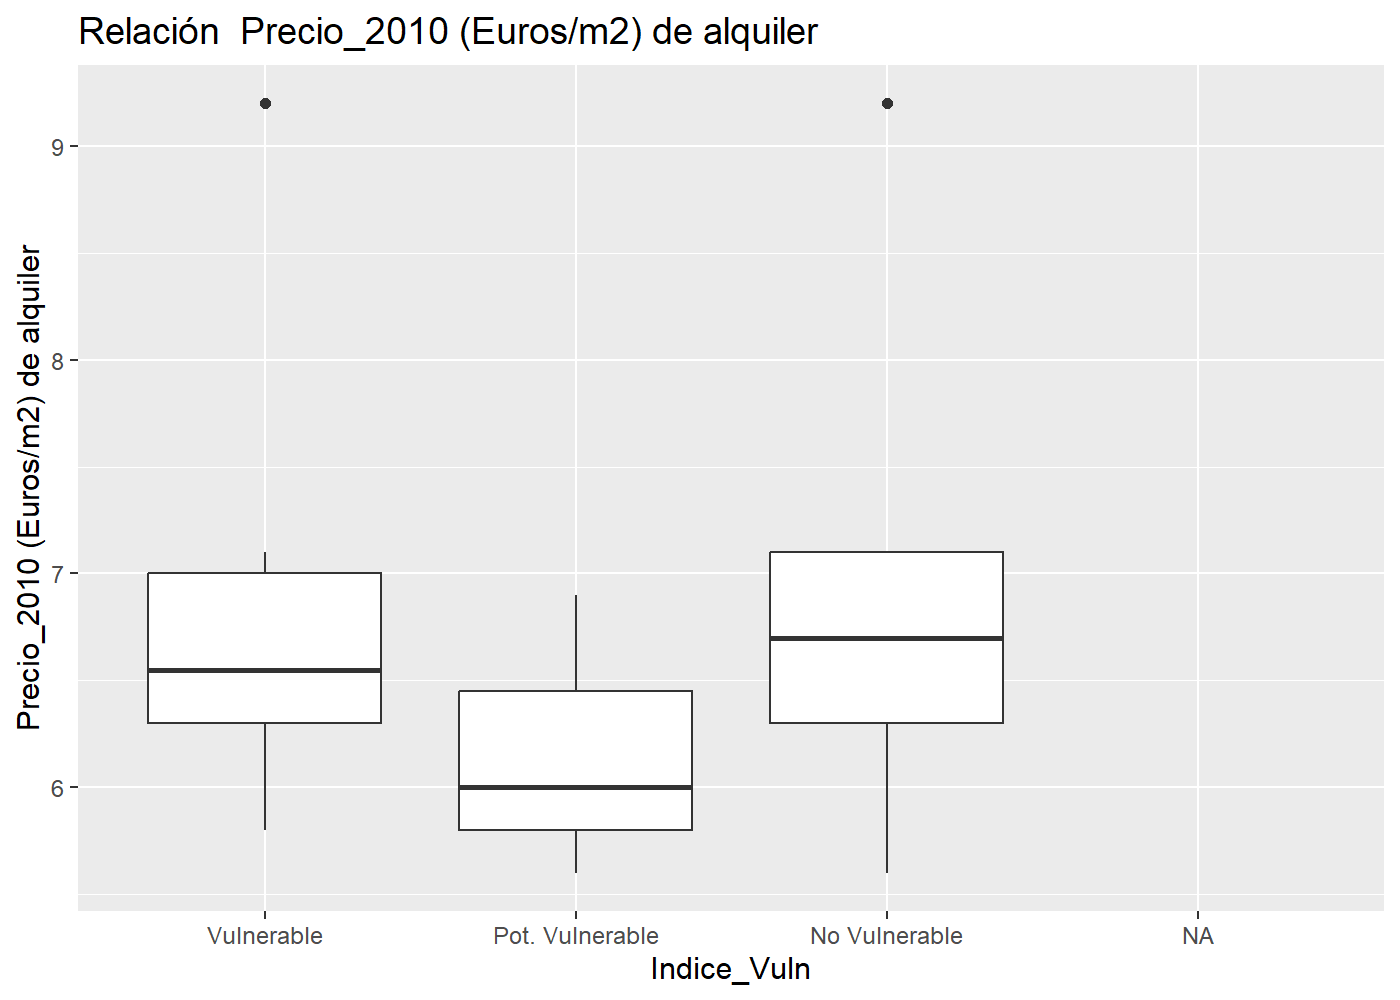
\includegraphics{./figure/unnamed-chunk-23-16} \end{center}

\begin{center}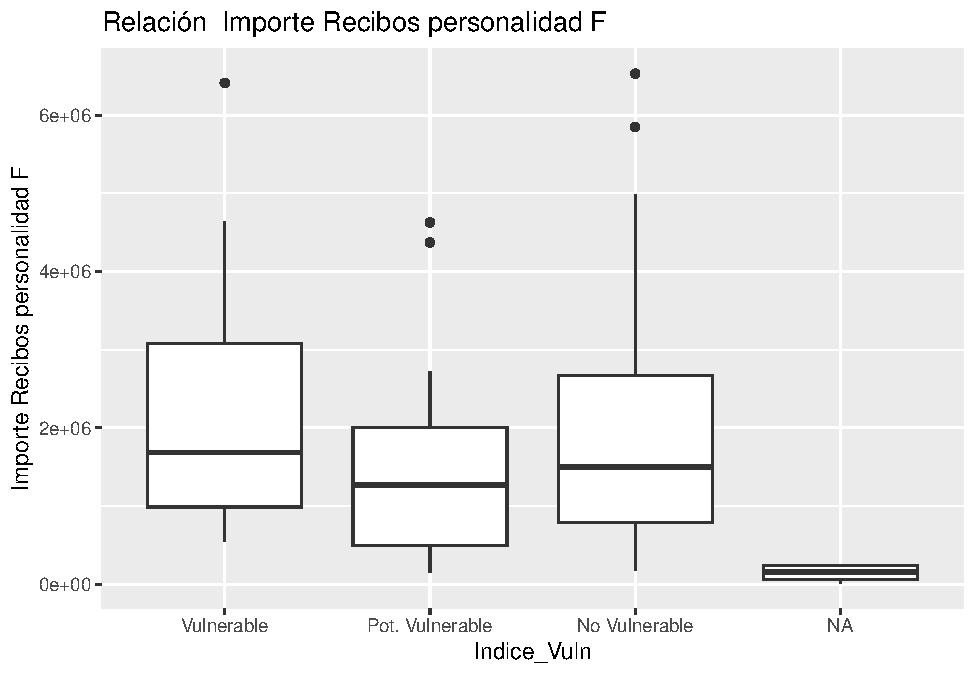
\includegraphics{./figure/unnamed-chunk-23-17} \end{center}

\begin{center}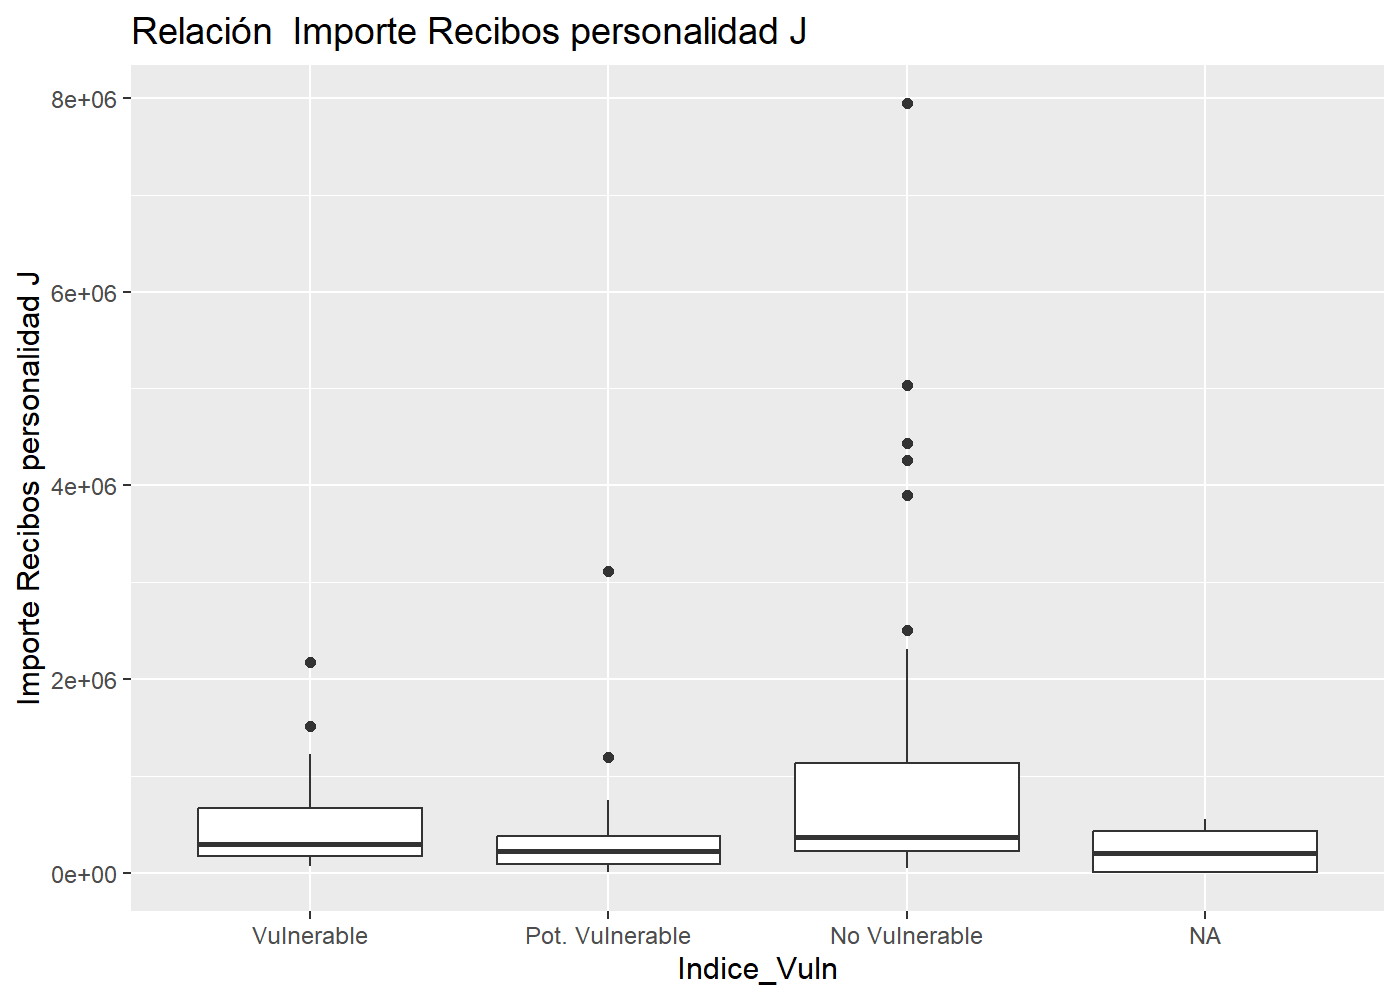
\includegraphics{./figure/unnamed-chunk-23-18} \end{center}

\begin{center}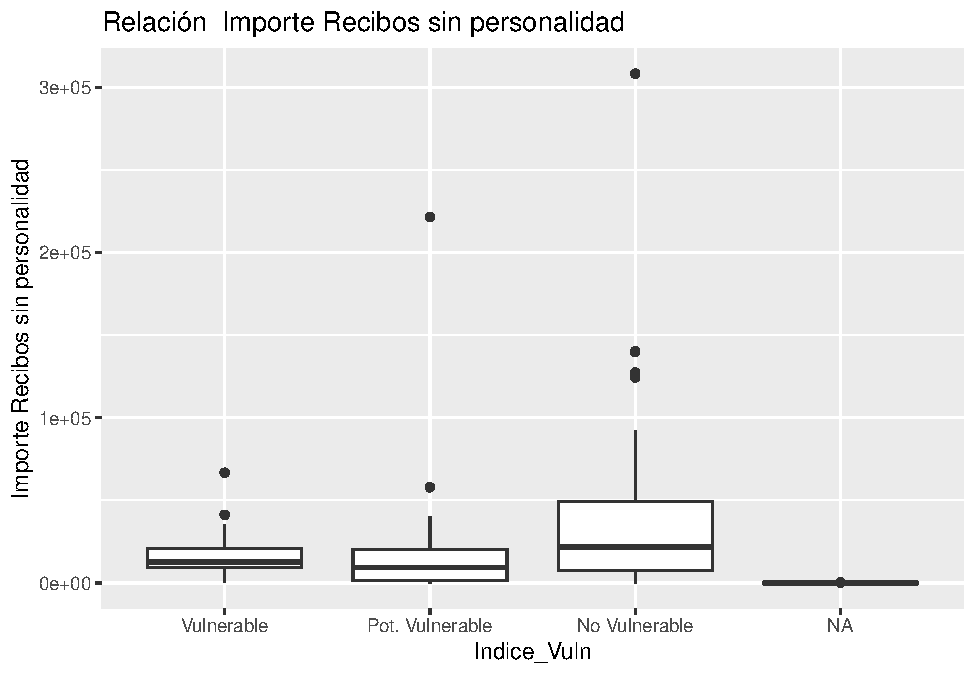
\includegraphics{./figure/unnamed-chunk-23-19} \end{center}

\begin{center}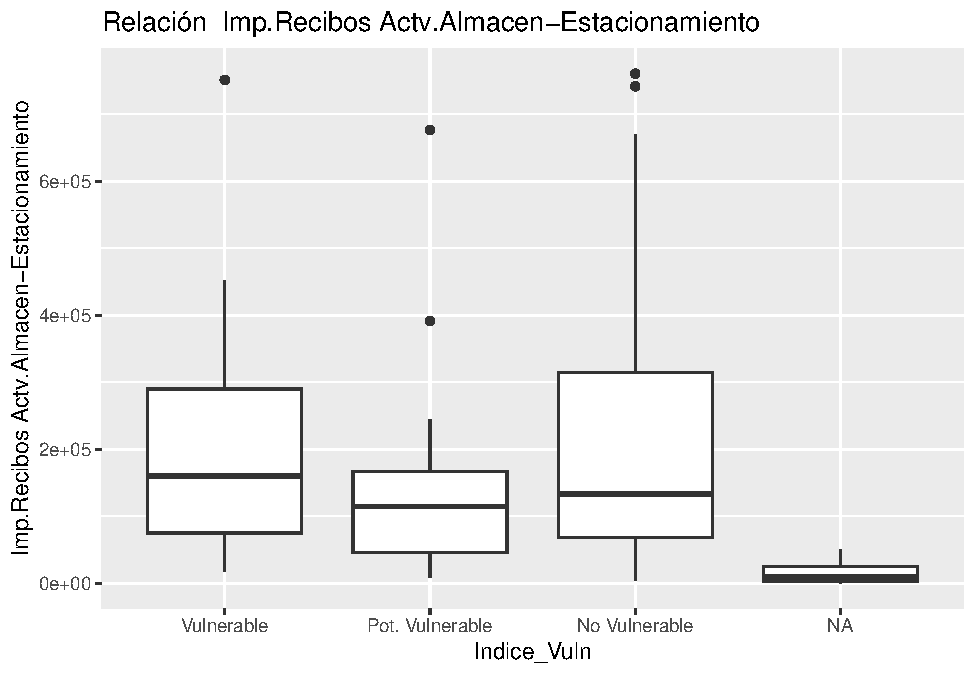
\includegraphics{./figure/unnamed-chunk-23-20} \end{center}

\begin{center}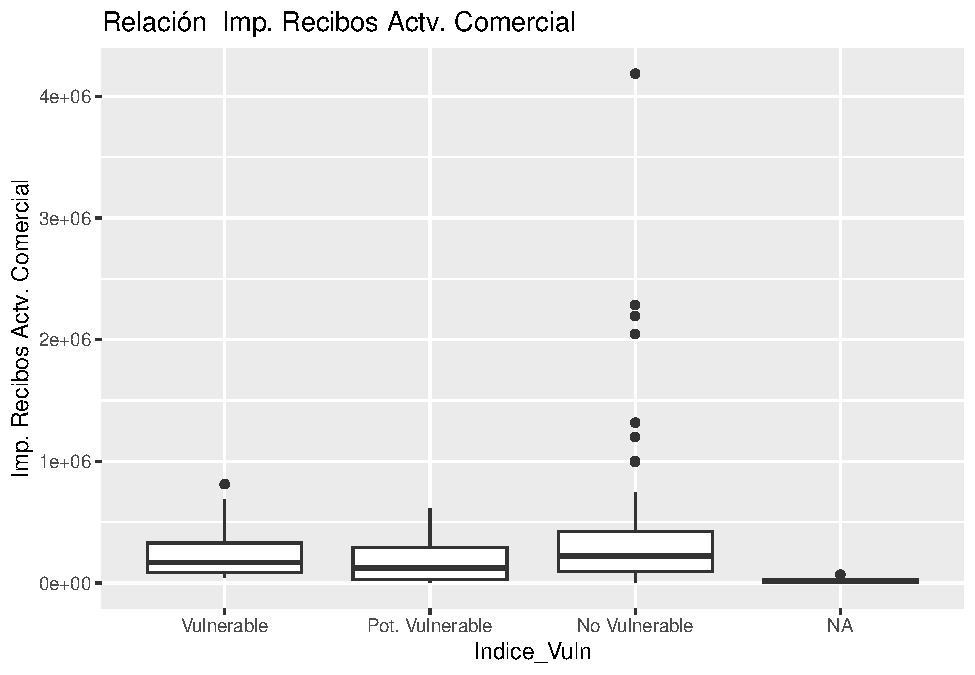
\includegraphics{./figure/unnamed-chunk-23-21} \end{center}

\begin{center}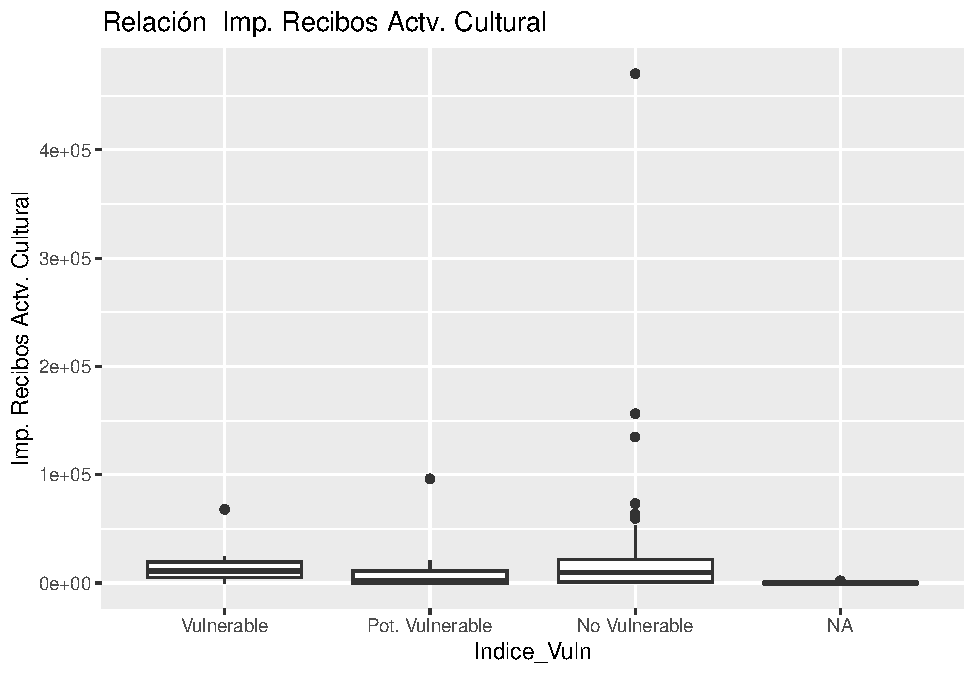
\includegraphics{./figure/unnamed-chunk-23-22} \end{center}

\begin{center}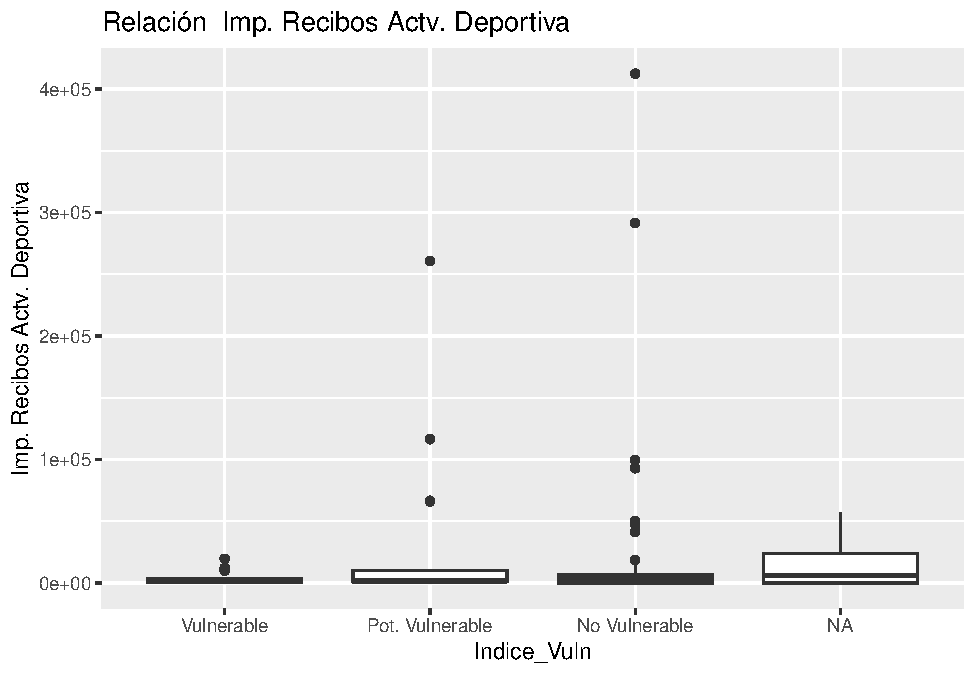
\includegraphics{./figure/unnamed-chunk-23-23} \end{center}

\begin{center}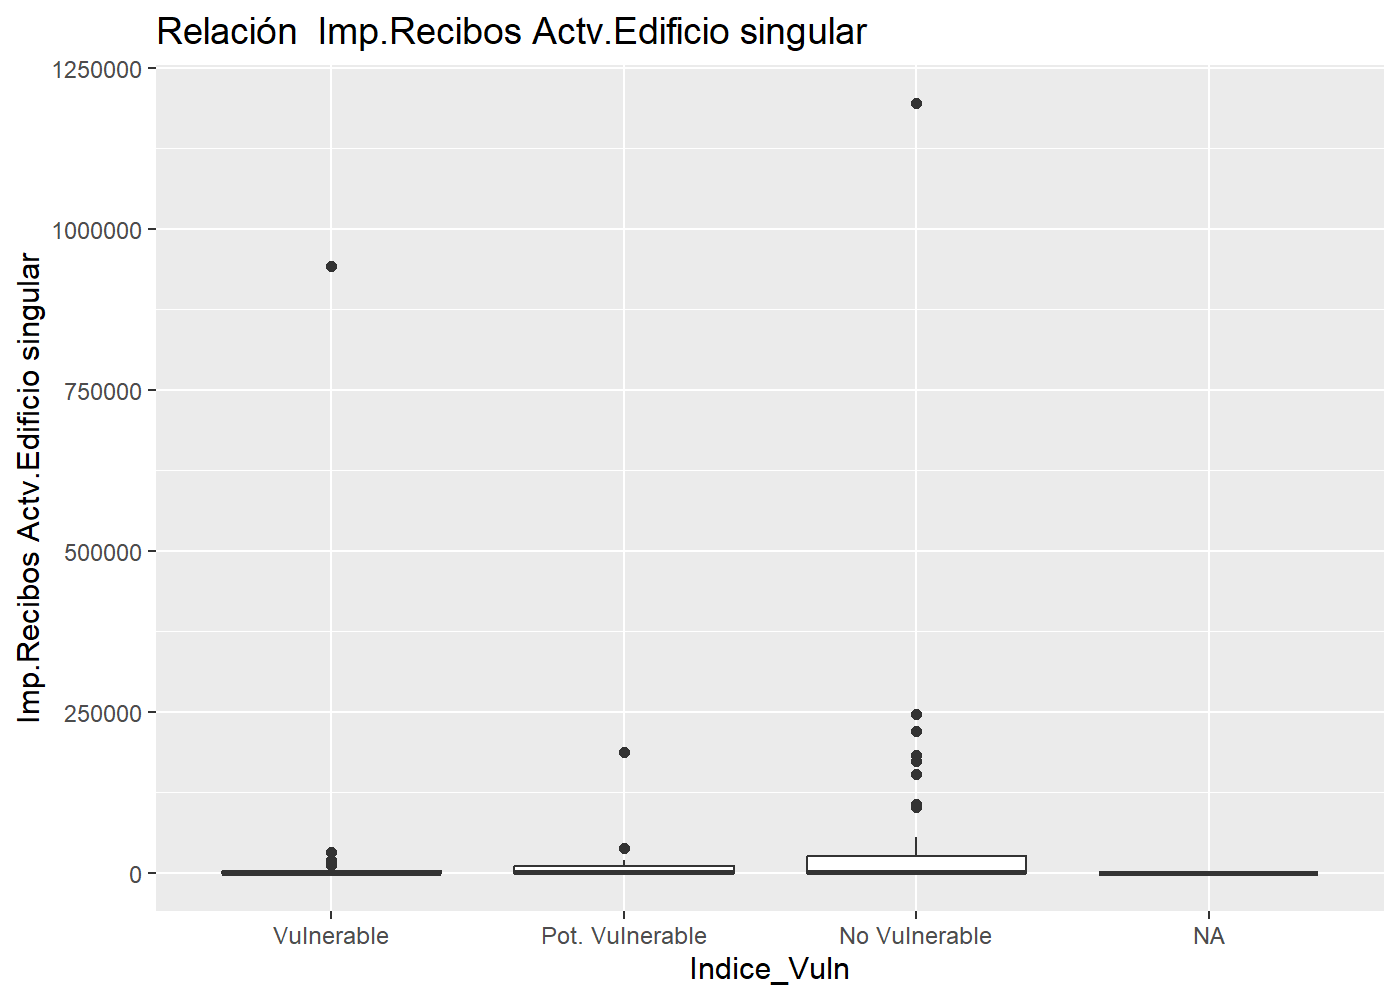
\includegraphics{./figure/unnamed-chunk-23-24} \end{center}

\begin{center}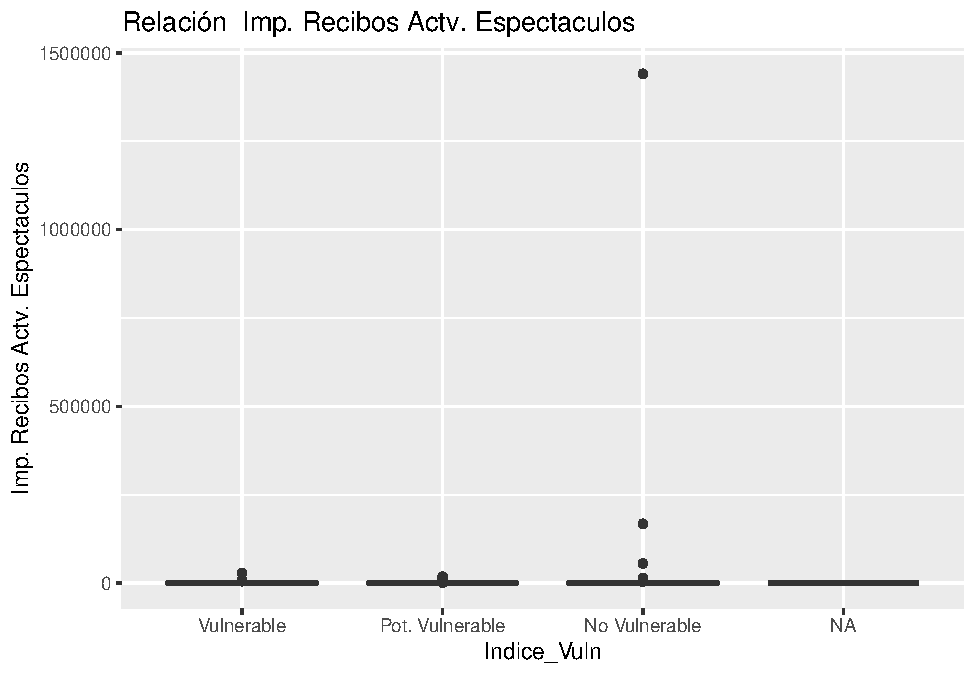
\includegraphics{./figure/unnamed-chunk-23-25} \end{center}

\begin{center}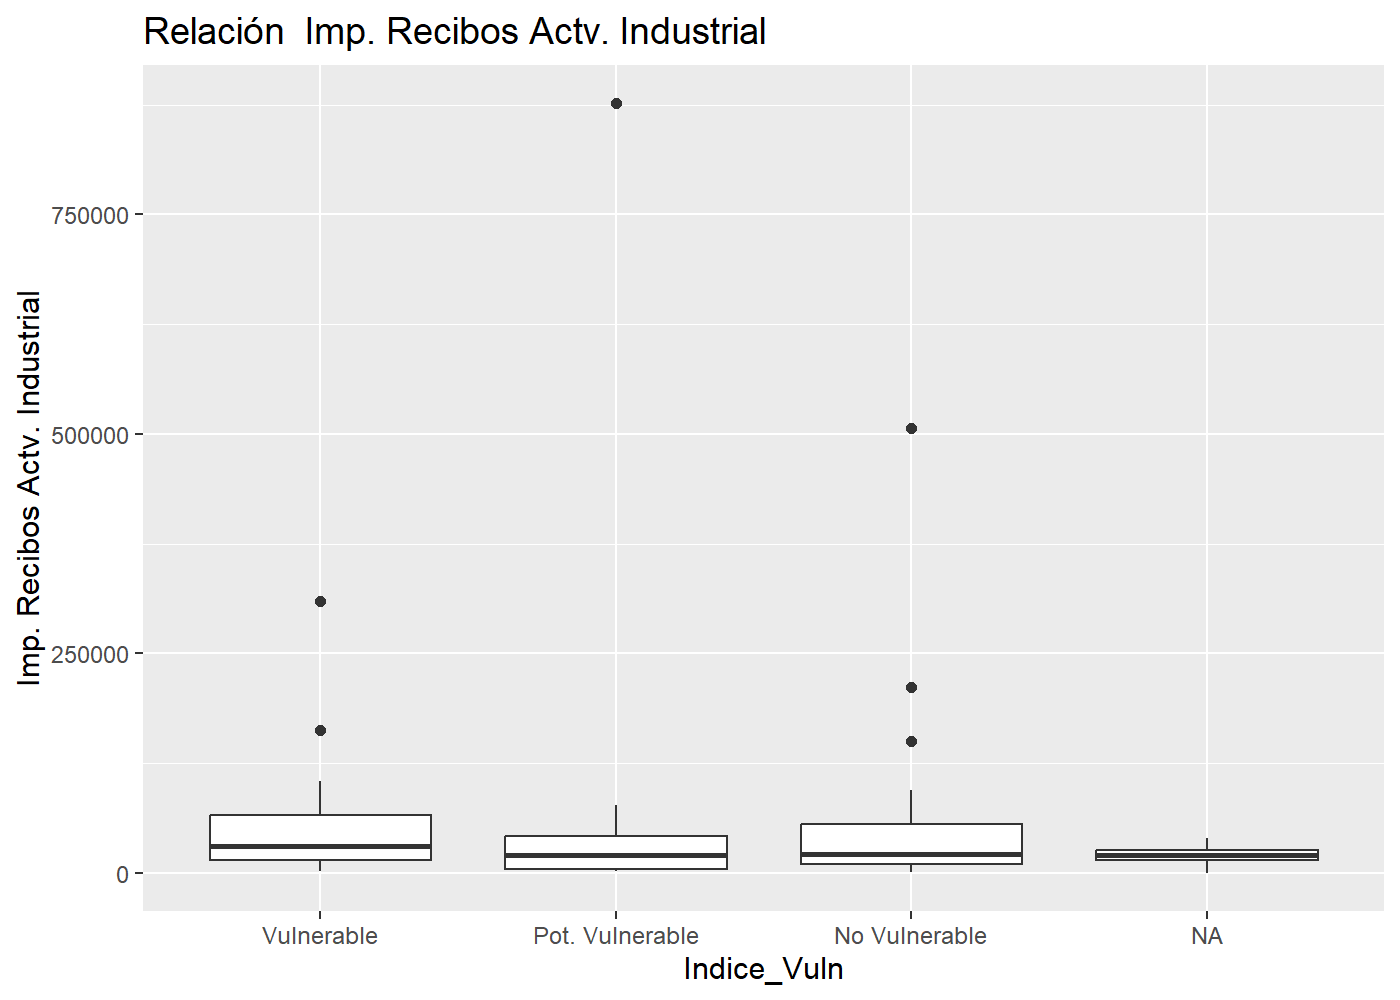
\includegraphics{./figure/unnamed-chunk-23-26} \end{center}

\begin{center}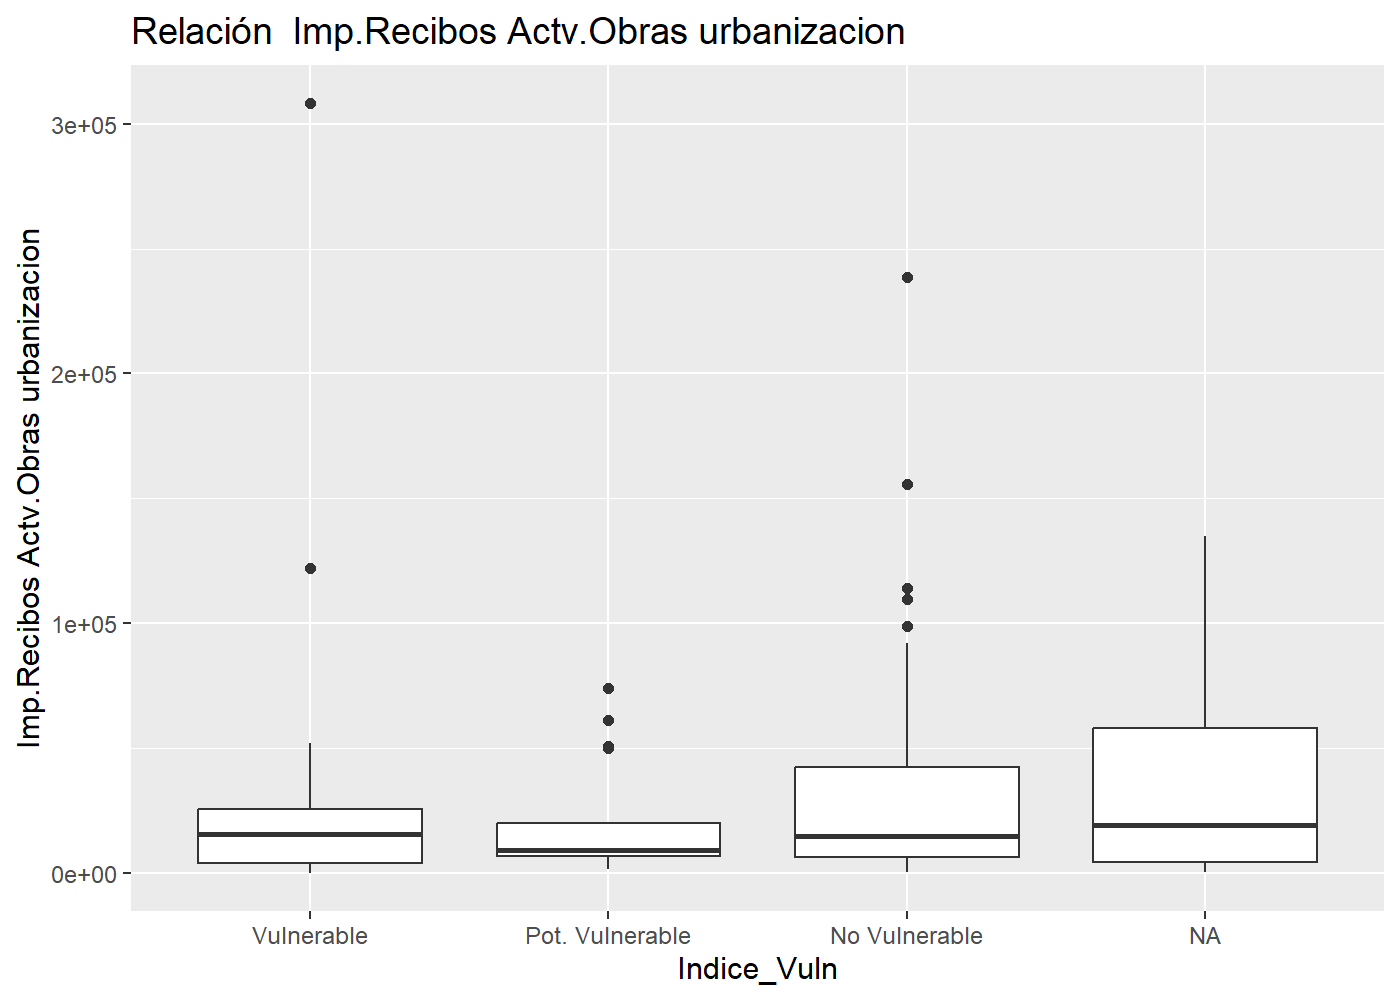
\includegraphics{./figure/unnamed-chunk-23-27} \end{center}

\begin{center}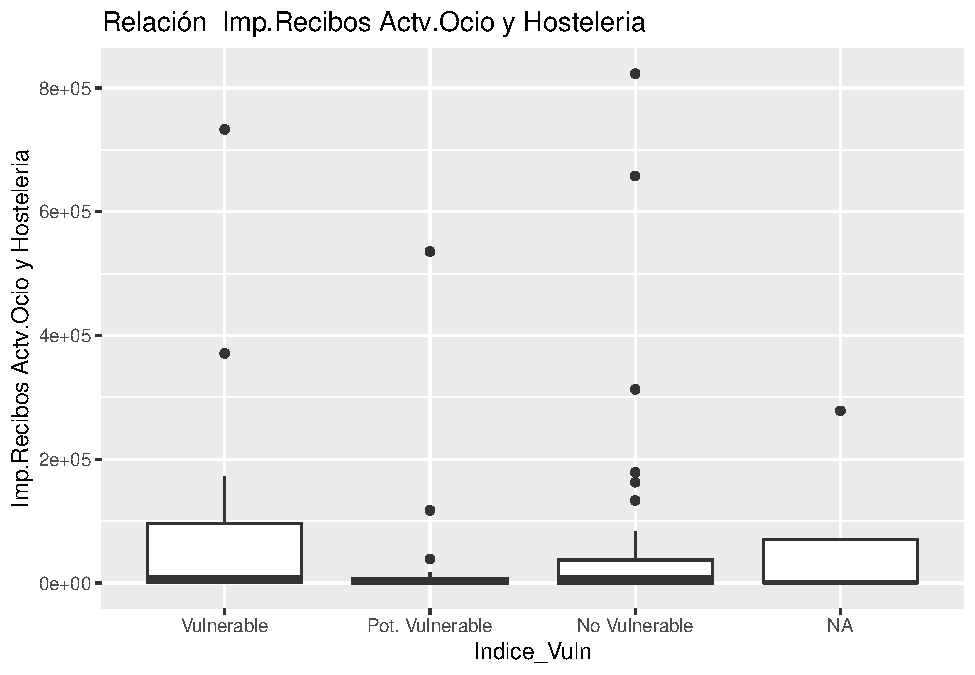
\includegraphics{./figure/unnamed-chunk-23-28} \end{center}

\begin{center}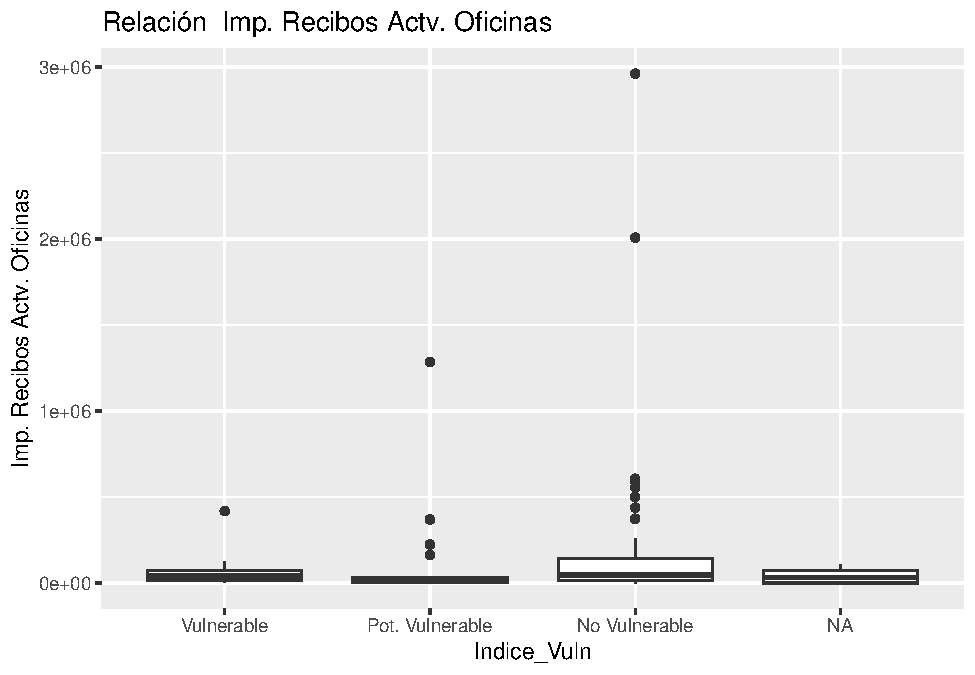
\includegraphics{./figure/unnamed-chunk-23-29} \end{center}

\begin{center}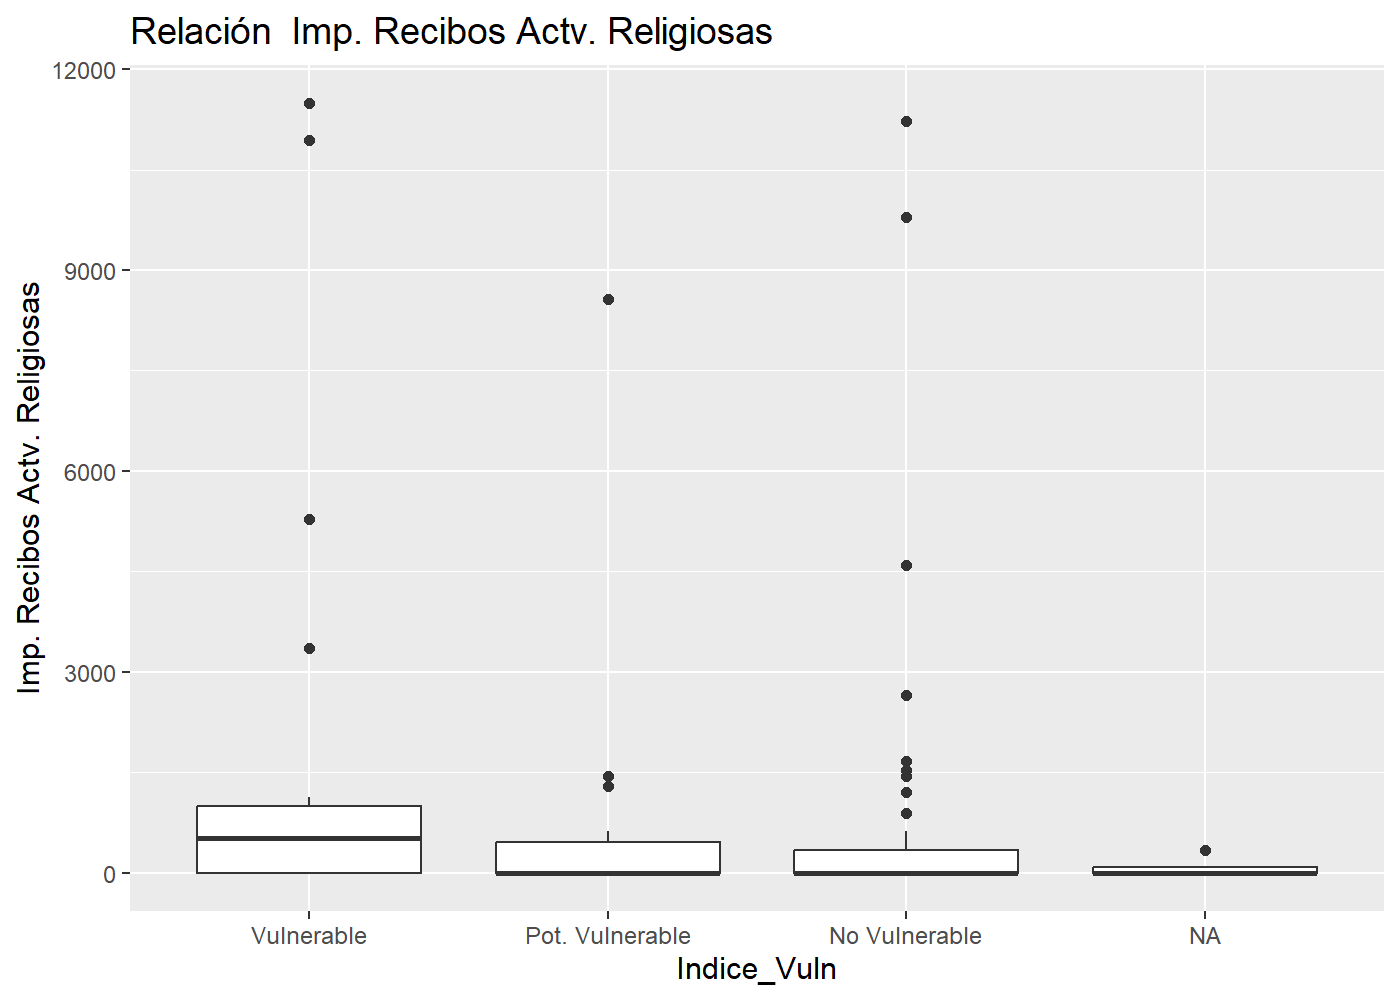
\includegraphics{./figure/unnamed-chunk-23-30} \end{center}

\begin{center}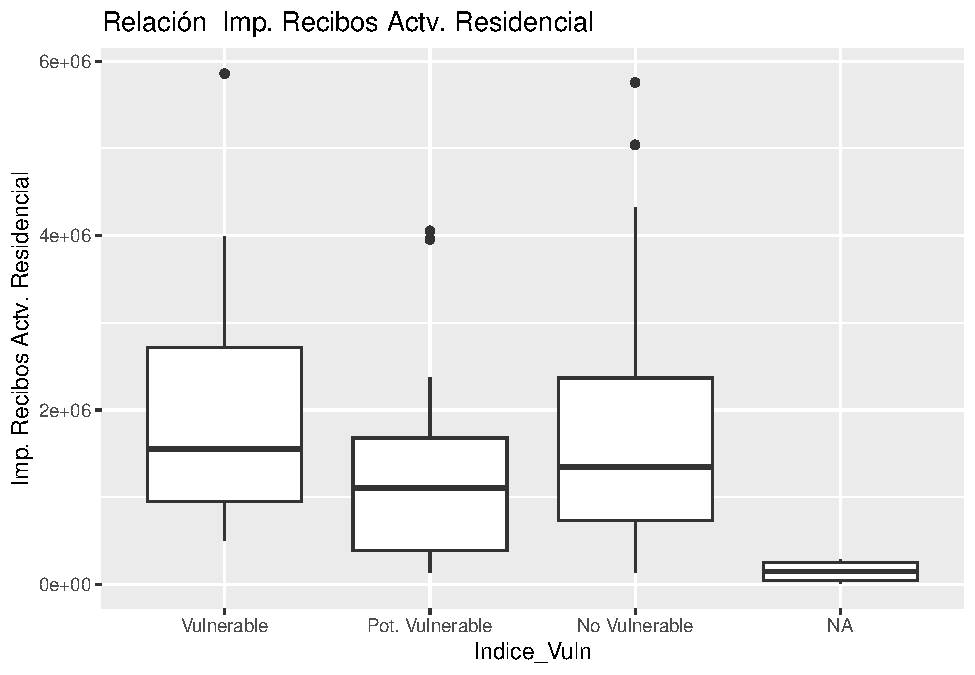
\includegraphics{./figure/unnamed-chunk-23-31} \end{center}

\begin{center}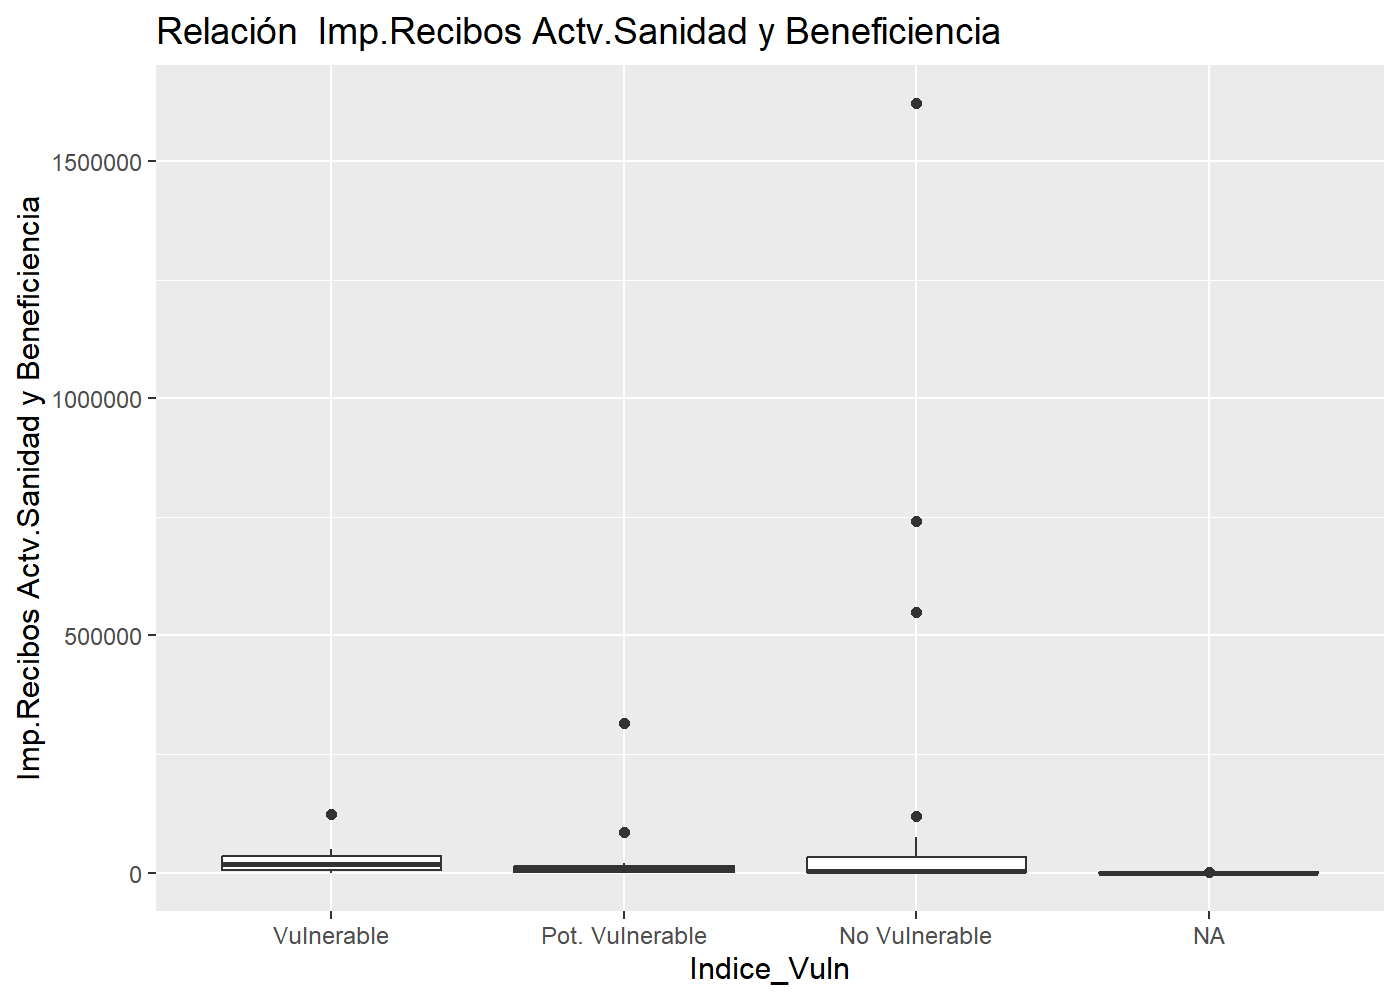
\includegraphics{./figure/unnamed-chunk-23-32} \end{center}

\begin{center}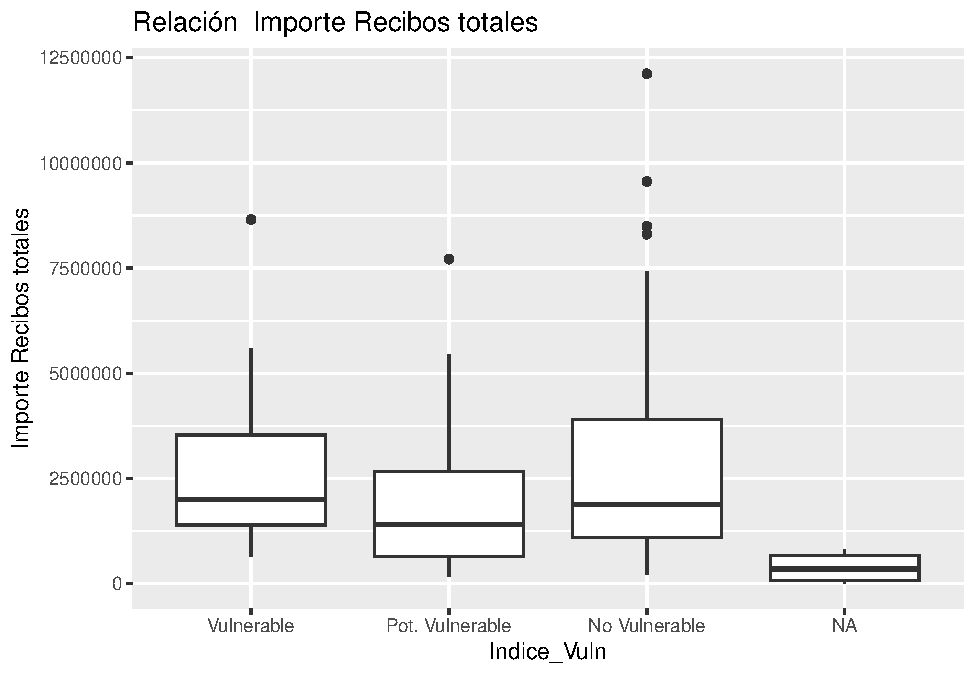
\includegraphics{./figure/unnamed-chunk-23-33} \end{center}

Una cosa que me ha interesado es ver si la diferencia del aumeto de
precio de compra en función de la vulnerabilidad

\hypertarget{detecciuxf3n-de-anomaluxedas}{%
\subsection{Detección de anomalías}\label{detecciuxf3n-de-anomaluxedas}}

\hypertarget{detecciuxf3n-de-valores-perdidos}{%
\subsubsection{Detección de valores
perdidos}\label{detecciuxf3n-de-valores-perdidos}}

Antes de tratar con nuestros datos, vamos a analizar la situación de
nuestro dataset. Primero, vamos a analizar los valores perdidos.

\begin{Shaded}
\begin{Highlighting}[]
\FunctionTok{aggr}\NormalTok{(df, }\AttributeTok{prop =} \ConstantTok{FALSE}\NormalTok{, }\AttributeTok{combined =} \ConstantTok{TRUE}\NormalTok{, }\AttributeTok{numbers =} \ConstantTok{TRUE}\NormalTok{, }\AttributeTok{sortVars =} \ConstantTok{TRUE}\NormalTok{, }\AttributeTok{sortCombs =} \ConstantTok{TRUE}\NormalTok{)}
\end{Highlighting}
\end{Shaded}

\begin{center}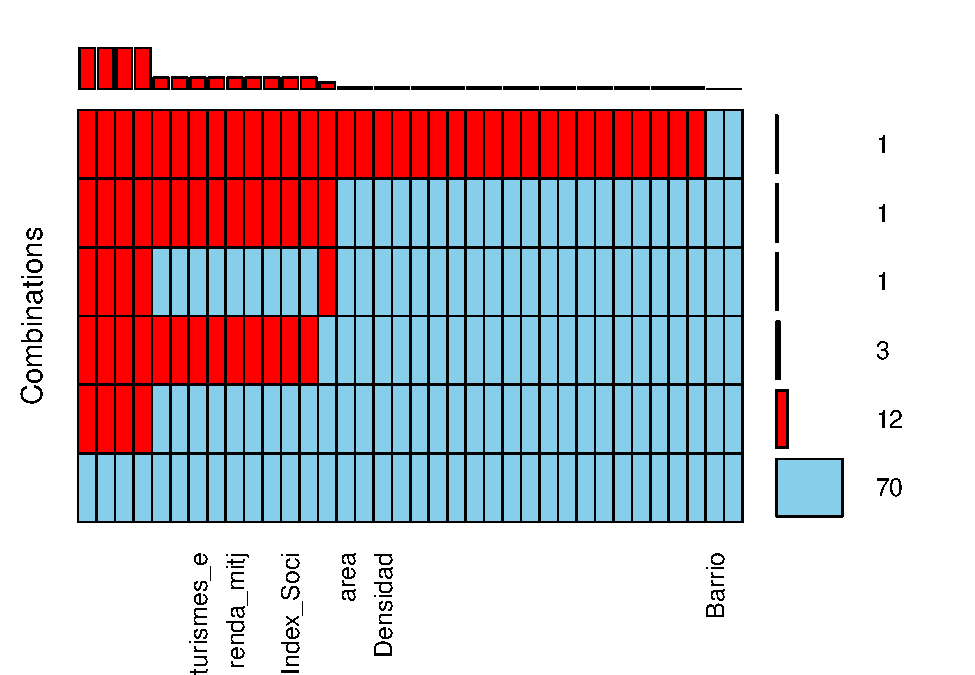
\includegraphics{./figure/unnamed-chunk-25-1} \end{center}

\begin{verbatim}

 Variables sorted by number of missings: 
                                 Variable Count
         Precio_2022 (Euros/m2) de compra    18
         Precio_2010 (Euros/m2) de compra    18
       Precio_2022 (Euros/m2) de alquiler    18
       Precio_2010 (Euros/m2) de alquiler    18
                              Indice_Vuln     5
                               Zones verd     5
                               turismes_e     5
                               atur_16_64     5
                               renda_mitj     5
                               risc_pobre     5
                               Index_Equi     5
                               Index_Soci     5
                               Index_Glob     5
                               Num_bancos     3
                                     area     1
                                poblacion     1
                                 Densidad     1
           Importe Recibos personalidad F     1
           Importe Recibos personalidad J     1
         Importe Recibos sin personalidad     1
 Imp.Recibos Actv.Almacen-Estacionamiento     1
             Imp. Recibos Actv. Comercial     1
              Imp. Recibos Actv. Cultural     1
             Imp. Recibos Actv. Deportiva     1
       Imp.Recibos Actv.Edificio singular     1
          Imp. Recibos Actv. Espectaculos     1
            Imp. Recibos Actv. Industrial     1
      Imp.Recibos Actv.Obras urbanizacion     1
       Imp.Recibos Actv.Ocio y Hosteleria     1
              Imp. Recibos Actv. Oficinas     1
            Imp. Recibos Actv. Religiosas     1
           Imp. Recibos Actv. Residencial     1
 Imp.Recibos Actv.Sanidad y Beneficiencia     1
                  Importe Recibos totales     1
                                   Barrio     0
                                 Distrito     0
\end{verbatim}

Este gráfico nos muestra las observaciones con valores perididos y en
qué columnas se hayan. Por ejemplo, para la primera observación, vemos
como todas las columnas a excepción de dos cuentan con un NA, y así
sucesivamente, hasta llegar a ver que hay 70 observaciones sin ningún
valor perdido.

\begin{Shaded}
\begin{Highlighting}[]
\FunctionTok{sum}\NormalTok{(}\FunctionTok{is.na}\NormalTok{(df))}
\end{Highlighting}
\end{Shaded}

\begin{verbatim}
[1] 140
\end{verbatim}

Podemos ver que la cantidad de valores perdidos en nuestro conjunto no
es precisamente pequeña, y principalmente se debe al hecho de que no
todos los conjuntos de datos que hemos fusionado contenían información
de todos los barrios, por lo que a la hora de unirlos todos se han
generado NAs en las observaciones donde no existían datos.

Una cosa que salta a la vista de las variables es esa observación que
cuenta con casi todos los valores peridos, que es la del barrio
``RAFALELL-VISTABELLA'', que no cuenta con ninguna información numérica
en nuestro dataset. Por ello, lo mejor que podemos hacer es eliminar la
observación.

\begin{Shaded}
\begin{Highlighting}[]
\NormalTok{df[df}\SpecialCharTok{$}\NormalTok{Barrio}\SpecialCharTok{==}\StringTok{"RAFALELL{-}VISTABELLA"}\NormalTok{,]}
\end{Highlighting}
\end{Shaded}

\begin{verbatim}
# A tibble: 1 x 36
  Barrio    Distrito Indice_Vuln `Zones verd` turismes_e atur_16_64 renda_mitj risc_pobre Index_Equi
  <fct>     <fct>    <fct>              <dbl>      <dbl>      <dbl>      <dbl>      <dbl>      <dbl>
1 RAFALELL~ POBLATS~ <NA>                  NA         NA         NA         NA         NA         NA
# i 27 more variables: Index_Soci <dbl>, Index_Glob <dbl>, area <dbl>, poblacion <dbl>,
#   Densidad <dbl>, Num_bancos <int>, `Precio_2022 (Euros/m2) de compra` <dbl>,
#   `Precio_2010 (Euros/m2) de compra` <dbl>, `Precio_2022 (Euros/m2) de alquiler` <dbl>,
#   `Precio_2010 (Euros/m2) de alquiler` <dbl>, `Importe Recibos personalidad F` <dbl>,
#   `Importe Recibos personalidad J` <dbl>, `Importe Recibos sin personalidad` <dbl>,
#   `Imp.Recibos Actv.Almacen-Estacionamiento` <dbl>, `Imp. Recibos Actv. Comercial` <dbl>,
#   `Imp. Recibos Actv. Cultural` <dbl>, `Imp. Recibos Actv. Deportiva` <dbl>, ...
\end{verbatim}

\begin{Shaded}
\begin{Highlighting}[]
\NormalTok{df}\SpecialCharTok{\%\textless{}\textgreater{}\%}\FunctionTok{drop\_na}\NormalTok{(}\StringTok{"Importe Recibos personalidad F"}\NormalTok{)}

\FunctionTok{summary}\NormalTok{(df)}
\end{Highlighting}
\end{Shaded}

\begin{verbatim}
         Barrio               Distrito           Indice_Vuln   Zones verd       turismes_e    
 AIORA      : 1   POBLATS DEL SUD : 8   Vulnerable     :19   Min.   : 120.0   Min.   :  9.04  
 ALBORS     : 1   POBLATS DEL NORD: 7   Pot. Vulnerable:17   1st Qu.: 697.5   1st Qu.: 11.64  
 ARRANCAPINS: 1   QUATRE CARRERES : 7   No Vulnerable  :47   Median :1312.0   Median : 12.09  
 BENICALAP  : 1   CIUTAT VELLA    : 6   NA's           : 4   Mean   :1678.8   Mean   : 15.34  
 BENIFARAIG : 1   CAMINS AL GRAU  : 5                        3rd Qu.:2101.0   3rd Qu.: 12.55  
 BENIFERRI  : 1   POBLATS MARITIMS: 5                        Max.   :6999.0   Max.   :117.21  
 (Other)    :81   (Other)         :49                        NA's   :4        NA's   :4       
   atur_16_64       renda_mitj      risc_pobre       Index_Equi      Index_Soci      Index_Glob   
 Min.   :  5.64   Min.   : 7145   Min.   :  7.10   Min.   :1.280   Min.   :1.220   Min.   :2.140  
 1st Qu.: 21.57   1st Qu.: 9933   1st Qu.: 17.18   1st Qu.:2.745   1st Qu.:2.560   1st Qu.:2.740  
 Median : 53.78   Median :11227   Median : 20.97   Median :2.970   Median :2.950   Median :3.040  
 Mean   : 71.57   Mean   :12390   Mean   : 26.47   Mean   :2.828   Mean   :3.077   Mean   :3.011  
 3rd Qu.:109.52   3rd Qu.:14484   3rd Qu.: 25.99   3rd Qu.:3.180   3rd Qu.:3.615   3rd Qu.:3.300  
 Max.   :300.97   Max.   :25795   Max.   :406.70   Max.   :3.650   Max.   :4.610   Max.   :3.700  
 NA's   :4        NA's   :4       NA's   :4        NA's   :4       NA's   :4       NA's   :4      
      area          poblacion        Densidad          Num_bancos    
 Min.   :  9.40   Min.   :   58   Min.   :  0.5426   Min.   :  4.00  
 1st Qu.: 32.65   1st Qu.: 3792   1st Qu.: 73.7938   1st Qu.: 23.00  
 Median : 49.70   Median : 7084   Median :174.2773   Median : 39.00  
 Mean   :111.22   Mean   : 9197   Mean   :184.1990   Mean   : 66.05  
 3rd Qu.:113.50   3rd Qu.:12005   3rd Qu.:296.7284   3rd Qu.: 78.00  
 Max.   :824.80   Max.   :41483   Max.   :529.1489   Max.   :347.00  
                                                     NA's   :2       
 Precio_2022 (Euros/m2) de compra Precio_2010 (Euros/m2) de compra
 Min.   :1103                     Min.   :1162                    
 1st Qu.:1619                     1st Qu.:1408                    
 Median :1948                     Median :1782                    
 Mean   :2109                     Mean   :1748                    
 3rd Qu.:2558                     3rd Qu.:2098                    
 Max.   :4029                     Max.   :2455                    
 NA's   :17                       NA's   :17                      
 Precio_2022 (Euros/m2) de alquiler Precio_2010 (Euros/m2) de alquiler
 Min.   : 3.00                      Min.   :5.600                     
 1st Qu.: 8.40                      1st Qu.:6.200                     
 Median : 9.20                      Median :6.700                     
 Mean   : 9.24                      Mean   :6.634                     
 3rd Qu.:10.00                      3rd Qu.:6.900                     
 Max.   :13.20                      Max.   :9.200                     
 NA's   :17                         NA's   :17                        
 Importe Recibos personalidad F Importe Recibos personalidad J Importe Recibos sin personalidad
 Min.   :  14482                Min.   :    512                Min.   :     0                  
 1st Qu.: 707677                1st Qu.: 144817                1st Qu.:  5953                  
 Median :1468509                Median : 318308                Median : 14309                  
 Mean   :1823852                Mean   : 792413                Mean   : 30351                  
 3rd Qu.:2564798                3rd Qu.: 754960                3rd Qu.: 35682                  
 Max.   :6530900                Max.   :7943384                Max.   :308299                  
                                                                                               
 Imp.Recibos Actv.Almacen-Estacionamiento Imp. Recibos Actv. Comercial Imp. Recibos Actv. Cultural
 Min.   :   389.5                         Min.   :      0              Min.   :     0.0           
 1st Qu.: 54086.4                         1st Qu.:  63468              1st Qu.:   703.8           
 Median :119167.0                         Median : 171670              Median :  7528.8           
 Mean   :189466.3                         Mean   : 359646              Mean   : 21982.3           
 3rd Qu.:238521.2                         3rd Qu.: 342828              3rd Qu.: 20356.6           
 Max.   :760687.6                         Max.   :4185348              Max.   :470265.7           
                                                                                                  
 Imp. Recibos Actv. Deportiva Imp.Recibos Actv.Edificio singular Imp. Recibos Actv. Espectaculos
 Min.   :     0.0             Min.   :      0                    Min.   :      0.0              
 1st Qu.:   138.8             1st Qu.:      0                    1st Qu.:      0.0              
 Median :  2886.7             Median :    314                    Median :      0.0              
 Mean   : 21937.9             Mean   :  45151                    Mean   :  20467.7              
 3rd Qu.: 10138.5             3rd Qu.:  13372                    3rd Qu.:    962.7              
 Max.   :412291.6             Max.   :1194289                    Max.   :1441549.2              
                                                                                                
 Imp. Recibos Actv. Industrial Imp.Recibos Actv.Obras urbanizacion
 Min.   :   221.7              Min.   :     0                     
 1st Qu.:  8529.3              1st Qu.:  6080                     
 Median : 21832.9              Median : 13986                     
 Mean   : 52724.1              Mean   : 32175                     
 3rd Qu.: 50162.3              3rd Qu.: 38501                     
 Max.   :876392.3              Max.   :308183                     
                                                                  
 Imp.Recibos Actv.Ocio y Hosteleria Imp. Recibos Actv. Oficinas Imp. Recibos Actv. Religiosas
 Min.   :     0.0                   Min.   :      0             Min.   :    0.0              
 1st Qu.:   473.2                   1st Qu.:   7158             1st Qu.:    0.0              
 Median :  6140.9                   Median :  32072             Median :    0.0              
 Mean   : 63647.1                   Mean   : 158026             Mean   :  997.6              
 3rd Qu.: 37142.9                   3rd Qu.: 109142             3rd Qu.:  625.3              
 Max.   :823072.6                   Max.   :2961486             Max.   :11489.9              
                                                                                             
 Imp. Recibos Actv. Residencial Imp.Recibos Actv.Sanidad y Beneficiencia Importe Recibos totales
 Min.   :  14122                Min.   :      0                          Min.   :   14994       
 1st Qu.: 680254                1st Qu.:    310                          1st Qu.:  946959       
 Median :1312627                Median :   6381                          Median : 1841102       
 Mean   :1627169                Mean   :  53079                          Mean   : 2646641       
 3rd Qu.:2337007                3rd Qu.:  26475                          3rd Qu.: 3348840       
 Max.   :5857109                Max.   :1621880                          Max.   :12119614       
                                                                                                
\end{verbatim}

En el summary podemos ver que variables son las que cuentan con datos
perdidos, y por tanto las que debemos procesar.

Otra que resalta de las variables provenientes del dataset IBI es que
cuentan con un mínimo de 0, mientras que la media de los valores ronda
valores muy altos. Esto se puede deber a que hay ciertas actividades que
están presentes en un pequeño número de barrios, como los espectáculos o
la actividad religiosa. Dado que estos datos tienen sentido, vamos a
mantenerlos, ya que pasarlos a NA nos daría una media de estas
actividades totalmente irreal. En cambio, en el resto de variables, como
precios de alquiler y compra, y zonas verdes, si sería interesante
cambiar estos NA por la mediana de los barrios de su misma
vulnerabilidad, ya que estos NA si se pueden deber a una ausencia de
medición.

Además, dado que algunas columnas, como la de areas, tiene un gran
número de NA, podemos usar el estudio de correlaciones que hemos visto
anteriormente para sustituir el valor perdido por el equivalente en una
de las columnas correlacionadas (usando una regresión, por ejemplo). En
caso de tener un NA en la columna correlacionada, usaremos la mediana.
En el caso de los precios de compra de 2022, usaremos la renta media del
barrio, que cuentan con una correlación de 0.91:

\begin{Shaded}
\begin{Highlighting}[]
\NormalTok{reg}\OtherTok{\textless{}{-}}\FunctionTok{lm}\NormalTok{(}\StringTok{\textasciigrave{}}\AttributeTok{Precio\_2022 (Euros/m2) de compra}\StringTok{\textasciigrave{}}\SpecialCharTok{\textasciitilde{}}\NormalTok{renda\_mitj,df)}
  
\NormalTok{df}\SpecialCharTok{\%\textless{}\textgreater{}\%}\FunctionTok{mutate}\NormalTok{(}\StringTok{\textasciigrave{}}\AttributeTok{Precio\_2022 (Euros/m2) de compra}\StringTok{\textasciigrave{}}\OtherTok{=}\FunctionTok{ifelse}\NormalTok{(}\FunctionTok{is.na}\NormalTok{(}\StringTok{\textasciigrave{}}\AttributeTok{Precio\_2022 (Euros/m2) de compra}\StringTok{\textasciigrave{}}\NormalTok{)}\SpecialCharTok{\&!}\FunctionTok{is.na}\NormalTok{(renda\_mitj),reg}\SpecialCharTok{$}\NormalTok{coefficients[}\DecValTok{1}\NormalTok{]}\SpecialCharTok{+}\NormalTok{renda\_mitj}\SpecialCharTok{*}\NormalTok{reg}\SpecialCharTok{$}\NormalTok{coefficients[}\DecValTok{2}\NormalTok{],}\StringTok{\textasciigrave{}}\AttributeTok{Precio\_2022 (Euros/m2) de compra}\StringTok{\textasciigrave{}}\NormalTok{))}

\NormalTok{df }\SpecialCharTok{\%\textless{}\textgreater{}\%}
  \FunctionTok{group\_by}\NormalTok{(}\StringTok{\textasciigrave{}}\AttributeTok{Indice\_Vuln}\StringTok{\textasciigrave{}}\NormalTok{) }\SpecialCharTok{\%\textgreater{}\%} 
  \FunctionTok{mutate}\NormalTok{(}\StringTok{\textasciigrave{}}\AttributeTok{Precio\_2022 (Euros/m2) de compra}\StringTok{\textasciigrave{}}\OtherTok{=}\FunctionTok{ifelse}\NormalTok{(}\FunctionTok{is.na}\NormalTok{(}\StringTok{\textasciigrave{}}\AttributeTok{Precio\_2022 (Euros/m2) de compra}\StringTok{\textasciigrave{}}\NormalTok{),}\FunctionTok{median}\NormalTok{(}\StringTok{\textasciigrave{}}\AttributeTok{Precio\_2022 (Euros/m2) de compra}\StringTok{\textasciigrave{}}\NormalTok{,}\AttributeTok{na.rm =} \ConstantTok{TRUE}\NormalTok{),}\StringTok{\textasciigrave{}}\AttributeTok{Precio\_2022 (Euros/m2) de compra}\StringTok{\textasciigrave{}}\NormalTok{))}\SpecialCharTok{\%\textgreater{}\%}
  \FunctionTok{ungroup}\NormalTok{() }
\end{Highlighting}
\end{Shaded}

\begin{Shaded}
\begin{Highlighting}[]
\NormalTok{df }\SpecialCharTok{\%\textless{}\textgreater{}\%}
  \FunctionTok{group\_by}\NormalTok{(}\StringTok{\textasciigrave{}}\AttributeTok{Indice\_Vuln}\StringTok{\textasciigrave{}}\NormalTok{) }\SpecialCharTok{\%\textgreater{}\%} 
  \FunctionTok{mutate}\NormalTok{(}\StringTok{\textasciigrave{}}\AttributeTok{Precio\_2010 (Euros/m2) de compra}\StringTok{\textasciigrave{}}\OtherTok{=}\FunctionTok{ifelse}\NormalTok{(}\FunctionTok{is.na}\NormalTok{(}\StringTok{\textasciigrave{}}\AttributeTok{Precio\_2010 (Euros/m2) de compra}\StringTok{\textasciigrave{}}\NormalTok{),}\FunctionTok{median}\NormalTok{(}\StringTok{\textasciigrave{}}\AttributeTok{Precio\_2010 (Euros/m2) de compra}\StringTok{\textasciigrave{}}\NormalTok{,}\AttributeTok{na.rm =} \ConstantTok{TRUE}\NormalTok{),}\StringTok{\textasciigrave{}}\AttributeTok{Precio\_2010 (Euros/m2) de compra}\StringTok{\textasciigrave{}}\NormalTok{))}\SpecialCharTok{\%\textgreater{}\%}
  \FunctionTok{ungroup}\NormalTok{() }
\end{Highlighting}
\end{Shaded}

\begin{Shaded}
\begin{Highlighting}[]
\NormalTok{df }\SpecialCharTok{\%\textless{}\textgreater{}\%}
  \FunctionTok{group\_by}\NormalTok{(}\StringTok{\textasciigrave{}}\AttributeTok{Indice\_Vuln}\StringTok{\textasciigrave{}}\NormalTok{) }\SpecialCharTok{\%\textgreater{}\%} 
  \FunctionTok{mutate}\NormalTok{(}\StringTok{\textasciigrave{}}\AttributeTok{Precio\_2022 (Euros/m2) de alquiler}\StringTok{\textasciigrave{}}\OtherTok{=}\FunctionTok{ifelse}\NormalTok{(}\FunctionTok{is.na}\NormalTok{(}\StringTok{\textasciigrave{}}\AttributeTok{Precio\_2022 (Euros/m2) de alquiler}\StringTok{\textasciigrave{}}\NormalTok{),}\FunctionTok{median}\NormalTok{(}\StringTok{\textasciigrave{}}\AttributeTok{Precio\_2022 (Euros/m2) de alquiler}\StringTok{\textasciigrave{}}\NormalTok{,}\AttributeTok{na.rm =} \ConstantTok{TRUE}\NormalTok{),}\StringTok{\textasciigrave{}}\AttributeTok{Precio\_2022 (Euros/m2) de alquiler}\StringTok{\textasciigrave{}}\NormalTok{))}\SpecialCharTok{\%\textgreater{}\%}
  \FunctionTok{ungroup}\NormalTok{() }
\end{Highlighting}
\end{Shaded}

\begin{Shaded}
\begin{Highlighting}[]
\NormalTok{df }\SpecialCharTok{\%\textless{}\textgreater{}\%}
  \FunctionTok{group\_by}\NormalTok{(}\StringTok{\textasciigrave{}}\AttributeTok{Indice\_Vuln}\StringTok{\textasciigrave{}}\NormalTok{) }\SpecialCharTok{\%\textgreater{}\%} 
  \FunctionTok{mutate}\NormalTok{(}\StringTok{\textasciigrave{}}\AttributeTok{Precio\_2010 (Euros/m2) de alquiler}\StringTok{\textasciigrave{}}\OtherTok{=}\FunctionTok{ifelse}\NormalTok{(}\FunctionTok{is.na}\NormalTok{(}\StringTok{\textasciigrave{}}\AttributeTok{Precio\_2010 (Euros/m2) de alquiler}\StringTok{\textasciigrave{}}\NormalTok{),}\FunctionTok{median}\NormalTok{(}\StringTok{\textasciigrave{}}\AttributeTok{Precio\_2010 (Euros/m2) de alquiler}\StringTok{\textasciigrave{}}\NormalTok{,}\AttributeTok{na.rm =} \ConstantTok{TRUE}\NormalTok{),}\StringTok{\textasciigrave{}}\AttributeTok{Precio\_2010 (Euros/m2) de alquiler}\StringTok{\textasciigrave{}}\NormalTok{))}\SpecialCharTok{\%\textgreater{}\%}
  \FunctionTok{ungroup}\NormalTok{() }
\end{Highlighting}
\end{Shaded}

\begin{Shaded}
\begin{Highlighting}[]
\NormalTok{df }\SpecialCharTok{\%\textless{}\textgreater{}\%}
  \FunctionTok{group\_by}\NormalTok{(}\StringTok{\textasciigrave{}}\AttributeTok{Indice\_Vuln}\StringTok{\textasciigrave{}}\NormalTok{) }\SpecialCharTok{\%\textgreater{}\%} 
  \FunctionTok{mutate}\NormalTok{(}\StringTok{\textasciigrave{}}\AttributeTok{Num\_bancos}\StringTok{\textasciigrave{}}\OtherTok{=}\FunctionTok{ifelse}\NormalTok{(}\FunctionTok{is.na}\NormalTok{(}\StringTok{\textasciigrave{}}\AttributeTok{Num\_bancos}\StringTok{\textasciigrave{}}\NormalTok{),}\FunctionTok{median}\NormalTok{(}\StringTok{\textasciigrave{}}\AttributeTok{Num\_bancos}\StringTok{\textasciigrave{}}\NormalTok{,}\AttributeTok{na.rm =} \ConstantTok{TRUE}\NormalTok{),}\StringTok{\textasciigrave{}}\AttributeTok{Num\_bancos}\StringTok{\textasciigrave{}}\NormalTok{))}\SpecialCharTok{\%\textgreater{}\%}
  \FunctionTok{ungroup}\NormalTok{() }
\end{Highlighting}
\end{Shaded}

\begin{Shaded}
\begin{Highlighting}[]
\FunctionTok{aggr}\NormalTok{(df, }\AttributeTok{prop =} \ConstantTok{FALSE}\NormalTok{, }\AttributeTok{combined =} \ConstantTok{TRUE}\NormalTok{, }\AttributeTok{numbers =} \ConstantTok{TRUE}\NormalTok{, }\AttributeTok{sortVars =} \ConstantTok{TRUE}\NormalTok{, }\AttributeTok{sortCombs =} \ConstantTok{TRUE}\NormalTok{)}
\end{Highlighting}
\end{Shaded}

\begin{center}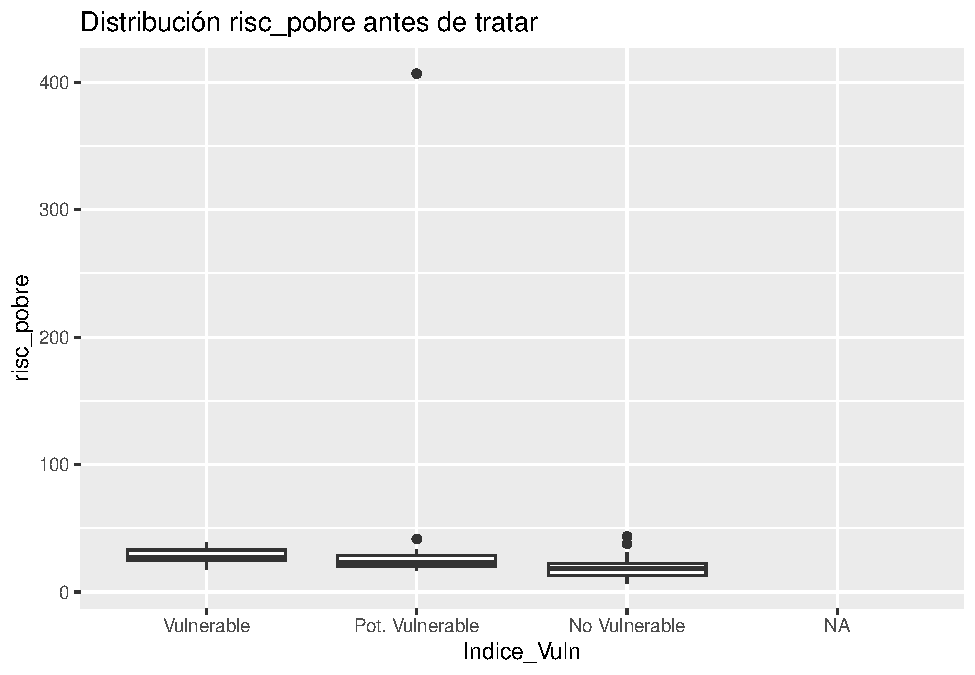
\includegraphics{./figure/unnamed-chunk-33-1} \end{center}

\begin{verbatim}

 Variables sorted by number of missings: 
                                 Variable Count
                              Indice_Vuln     4
                               Zones verd     4
                               turismes_e     4
                               atur_16_64     4
                               renda_mitj     4
                               risc_pobre     4
                               Index_Equi     4
                               Index_Soci     4
                               Index_Glob     4
         Precio_2022 (Euros/m2) de compra     4
         Precio_2010 (Euros/m2) de compra     4
       Precio_2022 (Euros/m2) de alquiler     4
       Precio_2010 (Euros/m2) de alquiler     4
                                   Barrio     0
                                 Distrito     0
                                     area     0
                                poblacion     0
                                 Densidad     0
                               Num_bancos     0
           Importe Recibos personalidad F     0
           Importe Recibos personalidad J     0
         Importe Recibos sin personalidad     0
 Imp.Recibos Actv.Almacen-Estacionamiento     0
             Imp. Recibos Actv. Comercial     0
              Imp. Recibos Actv. Cultural     0
             Imp. Recibos Actv. Deportiva     0
       Imp.Recibos Actv.Edificio singular     0
          Imp. Recibos Actv. Espectaculos     0
            Imp. Recibos Actv. Industrial     0
      Imp.Recibos Actv.Obras urbanizacion     0
       Imp.Recibos Actv.Ocio y Hosteleria     0
              Imp. Recibos Actv. Oficinas     0
            Imp. Recibos Actv. Religiosas     0
           Imp. Recibos Actv. Residencial     0
 Imp.Recibos Actv.Sanidad y Beneficiencia     0
                  Importe Recibos totales     0
\end{verbatim}

Tras esto hemos logrado pasar de tener un número muy elevado de NAs a
tener solo 4 en ciertas varibles. Estos NAs están en los barrios que
carecen de índice de vulverabilidad, por lo que tendremos que esperar a
ponerles una etiqueta a estos barrios para librarnos de los NAs de forma
adecuada.

\hypertarget{detecciuxf3n-de-outliers}{%
\subsubsection{Detección de outliers}\label{detecciuxf3n-de-outliers}}

Vamos a tratar los outliers de nuestro conjunto antes de empezar a
trabajar.

Para la detección de outliers vamos a usar los métodos 3-sigma y
boxplot, con las funciones definidas en la práctica 5.

\begin{Shaded}
\begin{Highlighting}[]
\NormalTok{reglasigma}\OtherTok{\textless{}{-}}\ControlFlowTok{function}\NormalTok{(x)\{}
\NormalTok{  x}\OtherTok{\textless{}{-}}\NormalTok{x[}\SpecialCharTok{!}\FunctionTok{is.na}\NormalTok{(x)}\SpecialCharTok{\&} \FunctionTok{is.numeric}\NormalTok{(x)]}
\NormalTok{  out }\OtherTok{\textless{}{-}} \FunctionTok{logical}\NormalTok{(}\FunctionTok{length}\NormalTok{(x)) }
  
  \ControlFlowTok{for}\NormalTok{(i }\ControlFlowTok{in} \DecValTok{1}\SpecialCharTok{:}\FunctionTok{length}\NormalTok{(x))\{}
    \ControlFlowTok{if}\NormalTok{(}\FunctionTok{abs}\NormalTok{(x[i]}\SpecialCharTok{{-}}\FunctionTok{mean}\NormalTok{(x))}\SpecialCharTok{\textgreater{}}\DecValTok{3}\SpecialCharTok{*}\FunctionTok{sd}\NormalTok{(x))\{}
\NormalTok{      out[i]}\OtherTok{\textless{}{-}}\ConstantTok{TRUE}
\NormalTok{    \}}
\NormalTok{  \}}
  \ControlFlowTok{if}\NormalTok{ (}\FunctionTok{all}\NormalTok{(}\SpecialCharTok{!}\NormalTok{out))\{}
    \FunctionTok{return}\NormalTok{(}\ConstantTok{NA}\NormalTok{)}
\NormalTok{  \} }\ControlFlowTok{else}\NormalTok{ \{}
    \FunctionTok{return}\NormalTok{(out)}
\NormalTok{  \}}
\NormalTok{\}}

\NormalTok{reglaboxplot}\OtherTok{\textless{}{-}}\ControlFlowTok{function}\NormalTok{(x)\{}
\NormalTok{  x}\OtherTok{\textless{}{-}}\NormalTok{x[}\SpecialCharTok{!}\FunctionTok{is.na}\NormalTok{(x)}\SpecialCharTok{\&} \FunctionTok{is.numeric}\NormalTok{(x)]}
\NormalTok{  out }\OtherTok{\textless{}{-}} \FunctionTok{logical}\NormalTok{(}\FunctionTok{length}\NormalTok{(x)) }
  
  \ControlFlowTok{for}\NormalTok{(i }\ControlFlowTok{in} \DecValTok{1}\SpecialCharTok{:}\FunctionTok{length}\NormalTok{(x))\{}
    \ControlFlowTok{if}\NormalTok{(x[i]}\SpecialCharTok{\textgreater{}}\FunctionTok{quantile}\NormalTok{(x,}\FloatTok{0.75}\NormalTok{)}\SpecialCharTok{+}\FloatTok{1.5}\SpecialCharTok{*}\FunctionTok{IQR}\NormalTok{(x))\{}
\NormalTok{      out[i]}\OtherTok{\textless{}{-}}\ConstantTok{TRUE}
\NormalTok{    \} }\ControlFlowTok{else} \ControlFlowTok{if}\NormalTok{ (x[i]}\SpecialCharTok{\textless{}}\FunctionTok{quantile}\NormalTok{(x,}\FloatTok{0.25}\NormalTok{)}\SpecialCharTok{{-}}\FloatTok{1.5}\SpecialCharTok{*}\FunctionTok{IQR}\NormalTok{(x))\{}
\NormalTok{      out[i]}\OtherTok{\textless{}{-}}\ConstantTok{TRUE}
\NormalTok{    \}}
\NormalTok{  \}}
  \ControlFlowTok{if}\NormalTok{ (}\FunctionTok{all}\NormalTok{(}\SpecialCharTok{!}\NormalTok{out))\{}
    \FunctionTok{return}\NormalTok{(}\ConstantTok{NA}\NormalTok{)}
\NormalTok{  \} }\ControlFlowTok{else}\NormalTok{ \{}
    \FunctionTok{return}\NormalTok{(out)}
\NormalTok{  \}}
\NormalTok{\}}
\end{Highlighting}
\end{Shaded}

Vamos a poner un ejemplo gráfico de otra forma de detectar ouliters. En
el caso de la variable \texttt{risc\_pobre}, el valor introducido para
el barrio de Benimaclet, distaba 43.76 veces el rango intercuartílico de
la mediana de la distribución. Por tanto, se ha considerado un error de
\emph{input} y se le ha seleccionado un nuevo valor. Para ello, se ha
tenido en cuenta que el análisis que se ha realizado ha sido mediante
box-plots, donde se diferencian las distribuciones en función de la
varaible categórica \texttt{Indice\_Vuln}. Por tanto, para que no altere
esta gráfica, el valor de la observación de Benimaclet se ha sustituido
por la mediana correspondiente a la distribución con su misma
vulnerabilidad.

\begin{Shaded}
\begin{Highlighting}[]
\CommentTok{\# Corrección de outliers gráfica}
\FunctionTok{ggplot}\NormalTok{(df, }\FunctionTok{aes}\NormalTok{(}\AttributeTok{x =}\NormalTok{ Indice\_Vuln, }\AttributeTok{y =}\NormalTok{ risc\_pobre)) }\SpecialCharTok{+} \FunctionTok{geom\_boxplot}\NormalTok{() }\SpecialCharTok{+} \FunctionTok{ggtitle}\NormalTok{(}\StringTok{\textquotesingle{}Distribución risc\_pobre antes de tratar\textquotesingle{}}\NormalTok{)}
\end{Highlighting}
\end{Shaded}

\begin{center}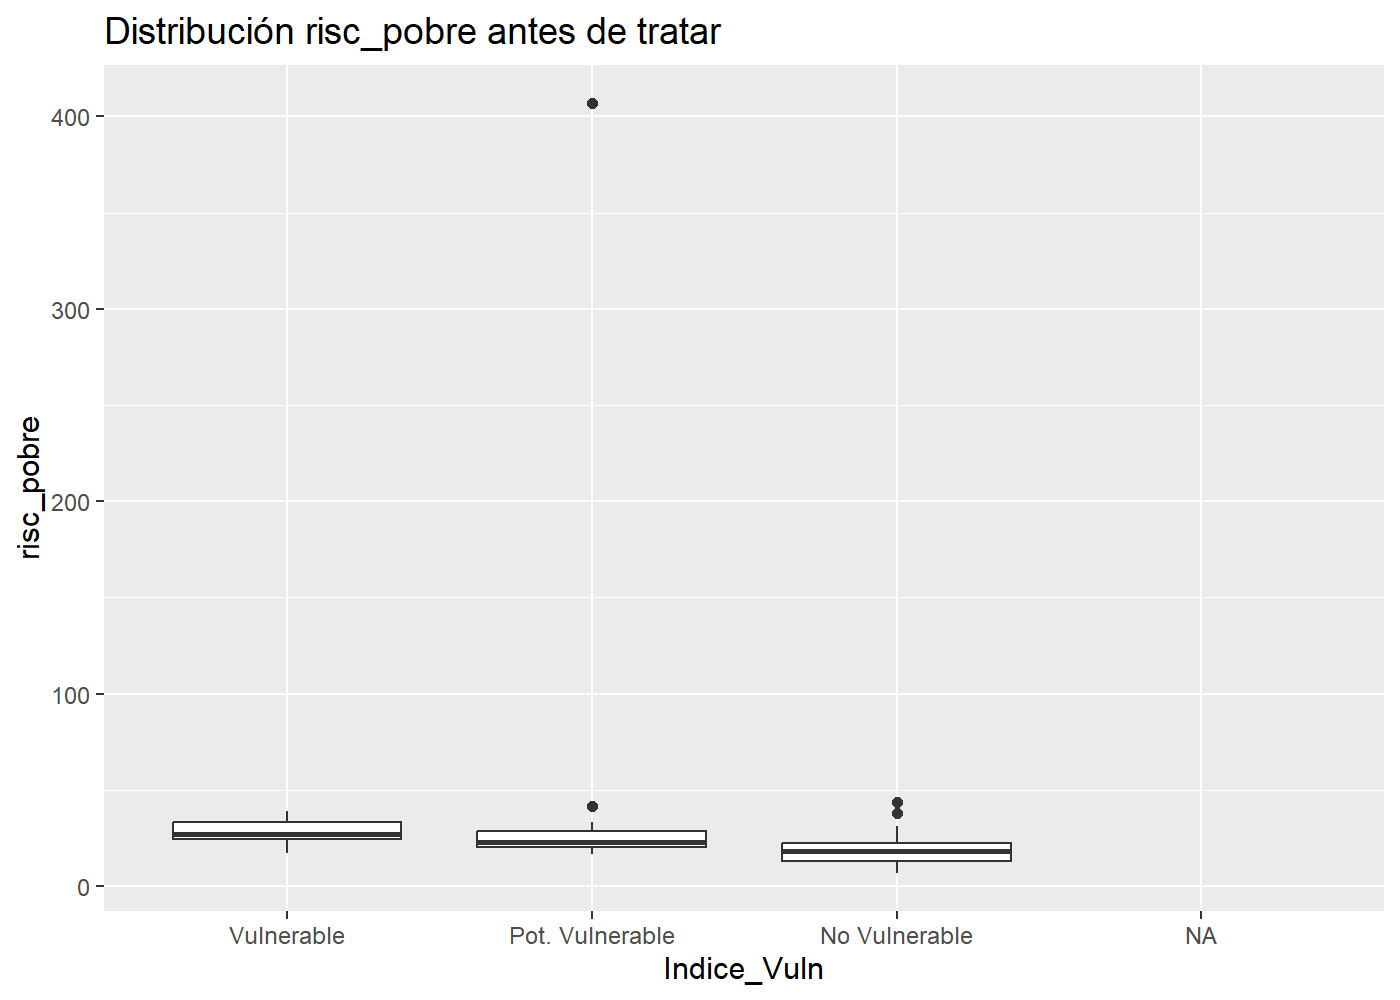
\includegraphics{./figure/unnamed-chunk-35-1} \end{center}

\begin{Shaded}
\begin{Highlighting}[]
\NormalTok{risc\_pobre\_filtrada }\OtherTok{\textless{}{-}}\NormalTok{ df }\SpecialCharTok{\%\textgreater{}\%}
  \FunctionTok{filter}\NormalTok{(Indice\_Vuln }\SpecialCharTok{==} \StringTok{\textquotesingle{}Vulnerable\textquotesingle{}}\NormalTok{) }\SpecialCharTok{\%\textgreater{}\%}
  \FunctionTok{filter}\NormalTok{(risc\_pobre }\SpecialCharTok{\textless{}} \DecValTok{100}\NormalTok{) }\SpecialCharTok{\%\textgreater{}\%}
  \FunctionTok{select}\NormalTok{(risc\_pobre)}
\NormalTok{df}\SpecialCharTok{$}\NormalTok{risc\_pobre[df[}\StringTok{\textquotesingle{}Barrio\textquotesingle{}}\NormalTok{] }\SpecialCharTok{==} \StringTok{\textquotesingle{}BENIMACLET\textquotesingle{}}\NormalTok{] }\OtherTok{\textless{}{-}} \FunctionTok{median}\NormalTok{(risc\_pobre\_filtrada[[}\DecValTok{1}\NormalTok{]])}

\FunctionTok{ggplot}\NormalTok{(df, }\FunctionTok{aes}\NormalTok{(}\AttributeTok{x =}\NormalTok{ Indice\_Vuln, }\AttributeTok{y =}\NormalTok{ risc\_pobre)) }\SpecialCharTok{+} \FunctionTok{geom\_boxplot}\NormalTok{() }\SpecialCharTok{+} \FunctionTok{ggtitle}\NormalTok{(}\StringTok{\textquotesingle{}Distribución risc\_pobre después de tratar\textquotesingle{}}\NormalTok{)}
\end{Highlighting}
\end{Shaded}

\begin{center}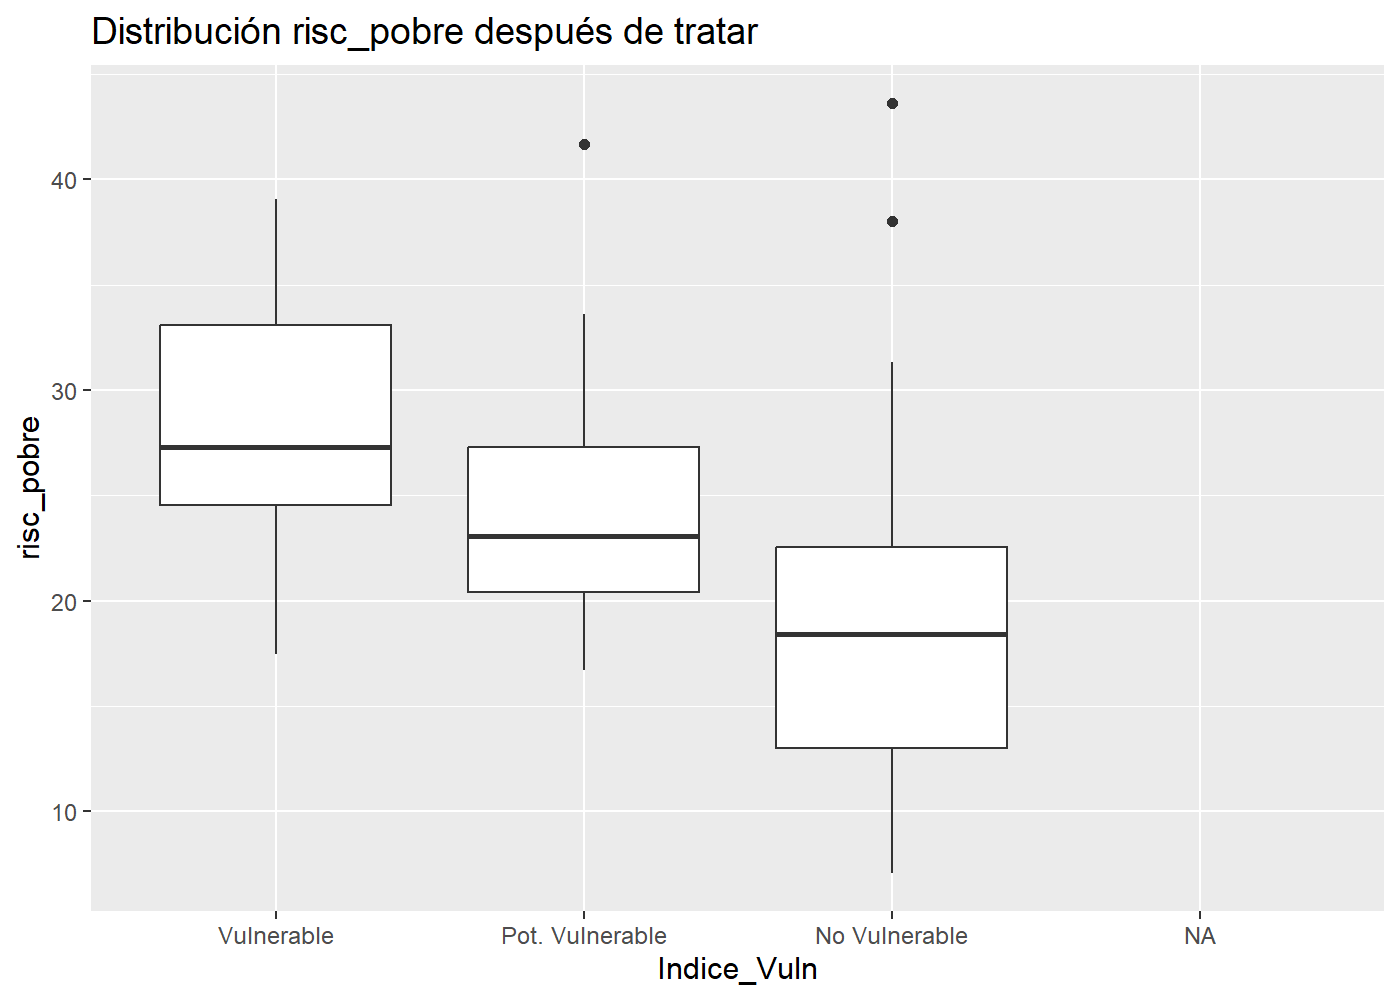
\includegraphics{./figure/unnamed-chunk-35-2} \end{center}

Para el resto de variables, vamos a aplicar las funciones vistas en
busca de posibles outliers.

\begin{Shaded}
\begin{Highlighting}[]
\NormalTok{outliers }\OtherTok{\textless{}{-}}\NormalTok{ df }\SpecialCharTok{\%\textgreater{}\%}
  \FunctionTok{summarise}\NormalTok{(}\FunctionTok{across}\NormalTok{(}\FunctionTok{where}\NormalTok{(is.numeric), }\FunctionTok{list}\NormalTok{(}\AttributeTok{Sigma =} \SpecialCharTok{\textasciitilde{}}\FunctionTok{sum}\NormalTok{(}\FunctionTok{reglasigma}\NormalTok{(.)), }\AttributeTok{Boxplot =} \SpecialCharTok{\textasciitilde{}}\FunctionTok{sum}\NormalTok{(}\FunctionTok{reglaboxplot}\NormalTok{(.))),}\AttributeTok{.names =} \StringTok{"\{col\};\{fn\}"}\NormalTok{))}

\NormalTok{outliers}\SpecialCharTok{\%\textless{}\textgreater{}\%}
  \FunctionTok{pivot\_longer}\NormalTok{(}\AttributeTok{cols=}\FunctionTok{everything}\NormalTok{(), }\AttributeTok{names\_to =} \StringTok{"Var"}\NormalTok{,}\AttributeTok{values\_to =} \StringTok{"Valor"}\NormalTok{)}\SpecialCharTok{\%\textgreater{}\%}
  \FunctionTok{separate}\NormalTok{(Var,}\AttributeTok{into=}\FunctionTok{c}\NormalTok{(}\StringTok{"Variable"}\NormalTok{, }\StringTok{"Regla"}\NormalTok{),}\AttributeTok{sep=}\StringTok{";"}\NormalTok{)}\SpecialCharTok{\%\textgreater{}\%}
  \FunctionTok{spread}\NormalTok{(}\AttributeTok{key=}\NormalTok{Regla,}\AttributeTok{value=}\NormalTok{Valor)}

\NormalTok{outliers}
\end{Highlighting}
\end{Shaded}

\begin{verbatim}
# A tibble: 33 x 3
   Variable                        Boxplot Sigma
   <chr>                             <int> <int>
 1 area                                 11     3
 2 atur_16_64                            2     1
 3 Densidad                             NA    NA
 4 Imp. Recibos Actv. Comercial          9     3
 5 Imp. Recibos Actv. Cultural          10     1
 6 Imp. Recibos Actv. Deportiva         13     3
 7 Imp. Recibos Actv. Espectaculos      16     1
 8 Imp. Recibos Actv. Industrial         6     2
 9 Imp. Recibos Actv. Oficinas          11     2
10 Imp. Recibos Actv. Religiosas        10     5
# i 23 more rows
\end{verbatim}

Viendo que la función boxplot detecta un número excesivo de outliers
contando las pocas observaciones que tenemos, vamos a hacer caso a la
regla sigma, y en caso de que haga falta modificar los outliers,
solamente trataremos los que esta detecta, pasandolos a la mediana al
igual que el ejemplo anterior, o usando alguna otra columna que esté muy
correlacionada.

Un ejemplo de outlier puede verse en la variable que muestra la
actividad cultural del barrio, viendo como la ciudad de las artes y las
ciencias tiene un valor muchísimo más alto que el resto:

\begin{Shaded}
\begin{Highlighting}[]
\NormalTok{p}\OtherTok{\textless{}{-}}\FunctionTok{ggplot}\NormalTok{(df[}\FunctionTok{c}\NormalTok{(}\StringTok{"Imp. Recibos Actv. Cultural"}\NormalTok{,}\StringTok{"Indice\_Vuln"}\NormalTok{)], }\FunctionTok{aes}\NormalTok{(}\AttributeTok{x =}\NormalTok{ Indice\_Vuln, }\AttributeTok{y =}\NormalTok{.data[[}\StringTok{"Imp. Recibos Actv. Cultural"}\NormalTok{]])) }\SpecialCharTok{+}
    \FunctionTok{geom\_boxplot}\NormalTok{() }\SpecialCharTok{+} 
    \FunctionTok{ggtitle}\NormalTok{(}\FunctionTok{paste}\NormalTok{(}\StringTok{"Relación con Imp. Recibos Actv. Cultural"}\NormalTok{))}
  \FunctionTok{print}\NormalTok{(p)}
\end{Highlighting}
\end{Shaded}

\begin{center}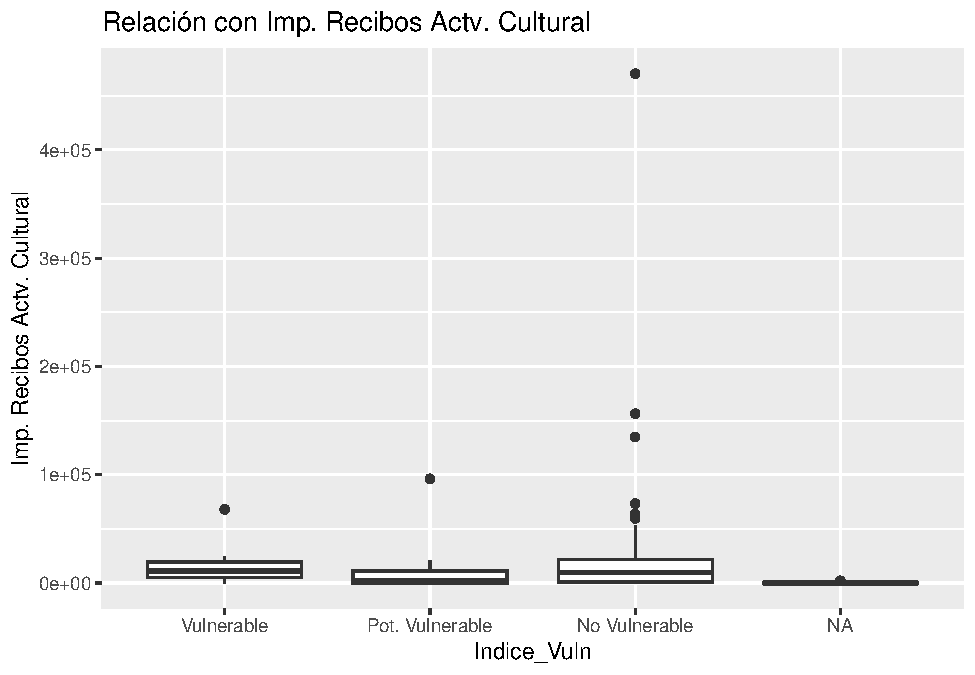
\includegraphics{./figure/unnamed-chunk-37-1} \end{center}

\begin{Shaded}
\begin{Highlighting}[]
  \FunctionTok{print}\NormalTok{(df}\SpecialCharTok{$}\StringTok{\textasciigrave{}}\AttributeTok{Imp. Recibos Actv. Cultural}\StringTok{\textasciigrave{}}\NormalTok{[df}\SpecialCharTok{$}\NormalTok{Barrio}\SpecialCharTok{==}\StringTok{"CIUTAT DE LES ARTS I DE LES CIENCIES"}\NormalTok{])}
\end{Highlighting}
\end{Shaded}

\begin{verbatim}
[1] 470265.7
\end{verbatim}

Vemos como dentro de los barrios no vulnerables el de la ciudad de las
artes y las ciencias tiene una actividad muchísimo mayor, con un valor
de 470265.7. Aun así, debido a que este dato no se debe a un error a la
hora de introducir el valor en el conjunto, pero se debe a que el barrio
tiene una actividad cultural mayor debido a su situación, mantendremos
estos outliers en nuestro dataset.

%%%%%%%%%%%%%%%%%%%%%%%%%%%%%%%%%%%%%%%%%%

\vspace{6pt}

%%%%%%%%%%%%%%%%%%%%%%%%%%%%%%%%%%%%%%%%%%
%% optional
\supplementary{The following supporting information can be downloaded
at:\\
\linksupplementary{s1}, Figure S1: title; Table S1: title; Video S1:
title.}

% Only for the journal Methods and Protocols:
% If you wish to submit a video article, please do so with any other supplementary material.
% \supplementary{The following supporting information can be downloaded at: \linksupplementary{s1}, Figure S1: title; Table S1: title; Video S1: title. A supporting video article is available at doi: link.}

%%%%%%%%%%%%%%%%%%%%%%%%%%%%%%%%%%%%%%%%%%
\authorcontributions{For research articles with several authors, a short
paragraph specifying their individual contributions must be provided.
The following statements should be used ``X.X. and Y.Y. conceive and
designed the experiments; X.X. performed the experiments; X.X. and Y.Y.
analyzed the data; W.W. contributed reagents/materials/analysis tools;
Y.Y. wrote the paper.'\,' Authorship must be limited to those who have
contributed substantially to the work reported.}

\funding{Please add:
\texttt{This\ research\ received\ no\ external\ funding\textquotesingle{}\textquotesingle{}\ or}This
research was funded by NAME OF FUNDER grant number XXX.'\,' and and
``The APC was funded by XXX'\,'. Check carefully that the details given
are accurate and use the standard spelling of funding agency names at
\url{https://search.crossref.org/funding}, any errors may affect your
future funding.}

\institutionalreview{In this section, you should add the Institutional
Review Board Statement and approval number, if relevant to your study.
You might choose to exclude this statement if the study did not require
ethical approval. Please note that the Editorial Office might ask you
for further information. Please add ``The study was conducted in
accordance with the Declaration of Helsinki, and approved by the
Institutional Review Board (or Ethics Committee) of NAME OF INSTITUTE
(protocol code XXX and date of approval).'' for studies involving
humans. OR ``The animal study protocol was approved by the Institutional
Review Board (or Ethics Committee) of NAME OF INSTITUTE (protocol code
XXX and date of approval).'' for studies involving animals. OR ``Ethical
review and approval were waived for this study due to REASON (please
provide a detailed justification).'' OR ``Not applicable'' for studies
not involving humans or animals.}

\informedconsent{Any research article describing a study involving
humans should contain this statement. Please add
\texttt{Informed\ consent\ was\ obtained\ from\ all\ subjects\ \ involved\ in\ the\ study.\textquotesingle{}\textquotesingle{}\ OR}Patient
consent was waived due to REASON (please provide a detailed
justification).'\,' OR ``Not applicable'\,' for studies not involving
humans. You might also choose to exclude this statement if the study did
not involve humans.

Written informed consent for publication must be obtained from
participating patients who can be identified (including by the patients
themselves). Please state ``Written informed consent has been obtained
from the patient(s) to publish this paper'\,' if applicable.}

\dataavailability{We encourage all authors of articles published in MDPI
journals to share their research data. In this section, please provide
details regarding where data supporting reported results can be found,
including links to publicly archived datasets analyzed or generated
during the study. Where no new data were created, or where data is
unavailable due to privacy or ethical re-strictions, a statement is
still required. Suggested Data Availability Statements are available in
section ``MDPI Research Data Policies'' at
\url{https://www.mdpi.com/ethics}.}

\acknowledgments{All sources of funding of the study should be
disclosed. Please clearly indicate grants that you have received in
support of your research work. Clearly state if you received funds for
covering the costs to publish in open access.}

\conflictsofinterest{Declare conflicts of interest or state `The authors
declare no conflict of interest.' Authors must identify and declare any
personal circumstances or interest that may be perceived as
inappropriately influencing the representation or interpretation of
reported research results. Any role of the funding sponsors in the
design of the study; in the collection, analyses or interpretation of
data in the writing of the manuscript, or in the decision to publish the
results must be declared in this section. If there is no role, please
state `The founding sponsors had no role in the design of the study; in
the collection, analyses, or interpretation of data; in the writing of
the manuscript, an in the decision to publish the results'.}

%%%%%%%%%%%%%%%%%%%%%%%%%%%%%%%%%%%%%%%%%%
%% Optional
\sampleavailability{Samples of the compounds \ldots\ldots{} are
available from the authors.}

%% Only for journal Encyclopedia

\abbreviations{Abbreviations}{
The following abbreviations are used in this manuscript:\\

\noindent
\begin{tabular}{@{}ll}
MDPI & Multidisciplinary Digital Publishing Institute \\
DOAJ & Directory of open access journals \\
TLA & Three letter acronym \\
LD & linear dichroism \\
\end{tabular}}

%%%%%%%%%%%%%%%%%%%%%%%%%%%%%%%%%%%%%%%%%%
%% Optional
\input{"appendix.tex"}
%%%%%%%%%%%%%%%%%%%%%%%%%%%%%%%%%%%%%%%%%%
\begin{adjustwidth}{-\extralength}{0cm}

%\printendnotes[custom] % Un-comment to print a list of endnotes


\reftitle{References}
\bibliography{mybibfile.bib}

% If authors have biography, please use the format below
%\section*{Short Biography of Authors}
%\bio
%{\raisebox{-0.35cm}{\includegraphics[width=3.5cm,height=5.3cm,clip,keepaspectratio]{Definitions/author1.pdf}}}
%{\textbf{Firstname Lastname} Biography of first author}
%
%\bio
%{\raisebox{-0.35cm}{\includegraphics[width=3.5cm,height=5.3cm,clip,keepaspectratio]{Definitions/author2.jpg}}}
%{\textbf{Firstname Lastname} Biography of second author}

%%%%%%%%%%%%%%%%%%%%%%%%%%%%%%%%%%%%%%%%%%
%% for journal Sci
%\reviewreports{\\
%Reviewer 1 comments and authors’ response\\
%Reviewer 2 comments and authors’ response\\
%Reviewer 3 comments and authors’ response
%}
%%%%%%%%%%%%%%%%%%%%%%%%%%%%%%%%%%%%%%%%%%
\PublishersNote{}
\end{adjustwidth}


\end{document}
